\documentclass[11pt]{article}
\usepackage[letterpaper,margin=0.7in]{geometry}
\usepackage[T1]{fontenc}
\usepackage{lmodern,booktabs,longtable,array,graphicx,tikz,xcolor,hyperref}
\usetikzlibrary{arrows.meta}
\definecolor{navy}{HTML}{16374A}
\definecolor{pale}{HTML}{EEF3F6}
\definecolor{amber}{HTML}{FFF4D6}
\definecolor{muted}{HTML}{576976}
\hypersetup{colorlinks=true,linkcolor=navy,urlcolor=navy,pdftitle={VCU Configuration and Modeling Control}}
\renewcommand{\familydefault}{\sfdefault}
\setlength{\parindent}{0pt}
\setlength{\parskip}{5pt}
\setlength{\emergencystretch}{3em}
\setcounter{tocdepth}{1}
\raggedbottom
\newcommand{\notebox}[1]{\par\noindent\colorbox{amber}{\parbox{\dimexpr\linewidth-2\fboxsep\relax}{#1}}\par}
\begin{document}
{\color{navy}\LARGE\bfseries VCU Configuration and\\[4pt] Modeling Control}\par
{\large Start here, evidence register and three sample forms}\par

\textbf{Configuration:} VCU-REV9-DRAFT-001\par
\notebox{\textbf{Draft for team completion.} The Rev9 geometry is a CAD candidate. Installed measurements and release approvals still need evidence.}
\section*{Start with one record}
You do not need to learn LaTeX to contribute. Open \textbf{inputs/VCU\_inputs.xlsx}, choose a Form tab, and fill the amber response cells. The package maintainer turns the saved workbook into this document and the labeled drawings.
\begin{enumerate}
\item \textbf{Choose one item.} Start with the upcomer pipe, the STC-02 sensor reference, or the insulation conductivity example.
\item \textbf{Read the reference.} Gray cells show what the supplied evidence says and where to find it. They are not confirmed answers.
\item \textbf{Enter what you know.} Add units, measurement date and the point or component you checked. Leave unknown values blank; add the open question in the evidence cell.
\item \textbf{Attach proof.} Name the file and the exact photo, page, row or certificate. Choose the evidence type and add your name/date.
\item \textbf{Return it for review.} The reviewer records the decision and its scope. Form entries do not automatically replace the baseline.
\end{enumerate}
\textbf{A useful first return:} one completed form, its evidence files, and a short list of anything you could not confirm. A partial, honest record is useful.
\textbf{Keep the example attached to its item.} To work on a different segment, sensor or material, save a separate response copy. Clear the old example references or have the maintainer replace them with evidence for the new item.
\textbf{Find your page:} pipe form p.~\pageref{form-pipe}; sensor form p.~\pageref{form-sensor}; property form p.~\pageref{form-material}; phase requests p.~\pageref{phase-requests}; complete requirements p.~\pageref{requirements}.
\textbf{Need help?} The repository file \textbf{START\_HERE.md} has separate paths for the experimental team, computational team and package maintainer.
\clearpage\section{Who fills in what?}
\textbf{Experimental team.} Record the installed hardware, fluids, sensor/channel mapping, calibration evidence, electrical wiring, coolant routing and raw logs. Use the phase requests to see what evidence is needed next.
\textbf{Computational team.} Propose model domains, boundary conditions, material correlations, uncertainty methods and validation checks. Explain the intended use and why each choice is suitable.
\textbf{Package reviewer.} Resolve conflicting evidence and record the approved choice, scope, date and effective configuration. The listed teams are suggested owners; named owners and release authority still need confirmation.
\textbf{Package maintainer.} Preserve the submitted evidence, update accepted input records deliberately, regenerate, and check that the document and diagrams match the saved workbook.
\subsection*{Two labels answer two different questions}
\small\setlength{\tabcolsep}{4pt}
\begin{longtable}{p{0.24\textwidth}p{0.68\textwidth}}
\toprule
\textbf{Evidence type} & \textbf{What it means} \\\midrule\endhead
CAD-derived & A result from the identified Rev9 model; installation not verified. \\[3pt]
Installed measurement & A measured physical item with date, method and evidence. \\[3pt]
Reported & A statement in notes or a communication; original evidence may still be needed. \\[3pt]
Modeling assumption & A proposed idealization or convention requiring rationale. \\[3pt]
Unknown & No supported value is available yet. \\[3pt]
\bottomrule\end{longtable}\normalsize
\textbf{Review state is separate:} Needs information, Needs review, Approved for stated use, or Not applicable with a reason. Approval must name the selected value, reviewer, date and scope. A CAD-derived value stays CAD-derived after review. This package establishes no approved physical or modeling choices.
\subsection*{What belongs in each package?}
\textbf{Configuration Control} describes the physical setup and measurement chain: geometry, insulation, fluids, instruments, calibration, heating/cooling, branch states and run identity.
\textbf{Modeling Control} describes how that setup is represented: 1-D and CFD/CHT domains, boundary/initial conditions, shared properties, closures, numerical checks, uncertainty and independent validation.
\textbf{Shared records} connect the two: evidence, approvals, sensor-to-model mapping, measured power, property selection and validation applicability.
\notebox{The STNCL documents are draft evidence sources. The requests in this package do not authorize running a test or establish that Nick Luciano has approved the draft requirements.}
\clearpage\tableofcontents
\clearpage\section{Configuration record and acceptance basis}\label{configuration-record}
\begingroup\small
The configuration record supplies the measured inputs and uncertainties needed to compare an experiment with a model. Record what changed, which evidence applies, and what error is acceptable for the stated comparison. Do not replace an unknown with a nominal value to complete the document.
\subsection*{Record identity}
\textbf{Facility:} VCU\par
\textbf{Configuration ID:} VCU-REV9-DRAFT-001\par
\textbf{Status:} Draft\par
\textbf{Scope:} Main-loop geometry and sensor-position prototype\par
\textbf{Geometry source:} VCU-R9-E01 (2026-10-08)\par
\textbf{Prepared by:} \textit{Unknown}\par
\textbf{Checked by:} \textit{Unknown}\par
\textbf{Plan approval:} Unconfirmed\par
\subsection*{Complete a dated package}
\small\setlength{\tabcolsep}{4pt}
\begin{longtable}{p{0.21\textwidth}p{0.28\textwidth}p{0.43\textwidth}}
\toprule
\textbf{Package item} & \textbf{Workbook record} & \textbf{Evidence to retain} \\\midrule\endhead
Identity and changes & Start; Requirements C01--C04 & Effective date, configuration ID, change history, reviewer and approved use. \\[3pt]
Geometry and insulation & Geometry; Form pipe; C05--C16 & Lengths, diameters, sensor datum, layer coverage, material certificates and measurement uncertainty. \\[3pt]
Photographs & Requirements C17 & Dated overview and detail files linked to the configuration, component and viewpoint. \\[3pt]
Fluids and properties & Fluids; Materials; Form material; C18--C20; M12--M19 & Product/composition, circuit, property source, equation, units, applicability and uncertainty. \\[3pt]
Instrumentation and calibration & Sensors; Calibration; Form sensor; C21--C33 & All instruments including fiber sensors: position, channel, certificate, correction, validity and uncertainty. \\[3pt]
Heater and cooler & Thermal spans; C34--C41 & Active boundaries, circuits, measured power/flow, calibration, feedback and setpoint history. \\[3pt]
Run and boundary state & Model choices; C42--C46 & Branches, tank/valve states, ambient conditions, operating limits, run ID and raw files. \\[3pt]
Model and acceptable error & Model choices; Requirements M01--M32 & Model revision, prediction targets, uncertainty method, conservation/convergence checks and quantitative acceptance limits. \\[3pt]
\bottomrule\end{longtable}\normalsize
\subsection*{Define what is good enough before comparison}
For each prediction target, record the quantity and units, applicable run/configuration, comparison interval, error metric, quantitative acceptance limit and uncertainty coverage. Explain how measurement and model uncertainty enter the decision. Use Requirements M01, M17 and M22--M32 for the selected choices and review scope; no numerical acceptance limits are supplied by this template.
\textbf{Where to enter evidence:} keep file/page/photo locators in the corresponding Requirements evidence fields. Use the selected choice, decision scope, reviewer/date and effective configuration fields for review decisions. The checklist above is a navigation aid, not a second editable record.
\par\endgroup
\clearpage\section{Pipe and insulation segment}\label{form-pipe}
Example: VCU upcomer B-C. Confirm the actual section before using the reported pipe or insulation details.
\par\textbf{Workbook tab:} Form pipe. Fill columns F--I. Every unanswered line below remains \textbf{TO CONFIRM}.
\textbf{Record context:} configuration / item / date / completed by: \hrulefill\par
\par\noindent\begin{minipage}{\textwidth}\small
{\color{navy}\bfseries Record identity}\hfill C01\par
\colorbox{pale}{\parbox{\dimexpr\linewidth-2\fboxsep\relax}{
\textbf{Reference only (CAD-derived):} VCU / upcomer / B-C\par
{\footnotesize Source: SEG upcomer row}}}\par
\textbf{Your entry:} {\color{muted}TO CONFIRM}\enspace\hrulefill\par
{\footnotesize\textbf{Evidence:} file + page/photo/row: \hrulefill\par
\textbf{Entry type / reviewer and date:} Unknown / Pending\par
}\end{minipage}\par\vspace{5pt}
\par\noindent\begin{minipage}{\textwidth}\small
{\color{navy}\bfseries Axis-end length (mm)}\hfill C06\par
\colorbox{pale}{\parbox{\dimexpr\linewidth-2\fboxsep\relax}{
\textbf{Reference only (CAD-derived):} 1219.200 mm\par
{\footnotesize Source: SEG upcomer reference\_\allowbreak{}length\_\allowbreak{}mm}}}\par
\textbf{Your entry:} {\color{muted}TO CONFIRM}\enspace\hrulefill\par
{\footnotesize\textbf{Evidence:} file + page/photo/row: \hrulefill\par
\textbf{Entry type / reviewer and date:} Unknown / Pending\par
}\end{minipage}\par\vspace{5pt}
\par\noindent\begin{minipage}{\textwidth}\small
{\color{navy}\bfseries Installed direction / tilt}\hfill C07\par
\colorbox{pale}{\parbox{\dimexpr\linewidth-2\fboxsep\relax}{
\textbf{Reference only (CAD-derived):} Vertical in CAD; phi = 0 deg from +y\par
{\footnotesize Source: SEG upcomer dx\_\allowbreak{}mm/dy\_\allowbreak{}mm}}}\par
\textbf{Your entry:} {\color{muted}TO CONFIRM}\enspace\hrulefill\par
{\footnotesize\textbf{Evidence:} file + page/photo/row: \hrulefill\par
\textbf{Entry type / reviewer and date:} Unknown / Pending\par
}\end{minipage}\par\vspace{5pt}
\par\noindent\begin{minipage}{\textwidth}\small
{\color{navy}\bfseries Inside diameter (mm)}\hfill C09\par
\colorbox{pale}{\parbox{\dimexpr\linewidth-2\fboxsep\relax}{
\textbf{Reference only (Reported):} CAD unknown. Notes: nominal 1.049 in (26.64 mm)\par
{\footnotesize Source: DIA Main swept loop; MAT lines 23-27}}}\par
\textbf{Your entry:} {\color{muted}TO CONFIRM}\enspace\hrulefill\par
{\footnotesize\textbf{Evidence:} file + page/photo/row: \hrulefill\par
\textbf{Entry type / reviewer and date:} Unknown / Pending\par
}\end{minipage}\par\vspace{5pt}
\par\noindent\begin{minipage}{\textwidth}\small
{\color{navy}\bfseries Outside diameter (mm)}\hfill C10\par
\colorbox{pale}{\parbox{\dimexpr\linewidth-2\fboxsep\relax}{
\textbf{Reference only (CAD-derived):} 33.401 mm\par
{\footnotesize Source: DIA Main swept loop}}}\par
\textbf{Your entry:} {\color{muted}TO CONFIRM}\enspace\hrulefill\par
{\footnotesize\textbf{Evidence:} file + page/photo/row: \hrulefill\par
\textbf{Entry type / reviewer and date:} Unknown / Pending\par
}\end{minipage}\par\vspace{5pt}
\clearpage
{\large\bfseries Pipe and insulation segment --- continued}\par
\textbf{Record context:} configuration / item / date: \hrulefill\par
\par\noindent\begin{minipage}{\textwidth}\small
{\color{navy}\bfseries Pipe grade / specification}\hfill C11\par
\colorbox{pale}{\parbox{\dimexpr\linewidth-2\fboxsep\relax}{
\textbf{Reference only (Reported):} 316L, nominal 1-inch schedule 40 reported\par
{\footnotesize Source: MAT lines 23-27}}}\par
\textbf{Your entry:} {\color{muted}TO CONFIRM}\enspace\hrulefill\par
{\footnotesize\textbf{Evidence:} file + page/photo/row: \hrulefill\par
\textbf{Entry type / reviewer and date:} Unknown / Pending\par
}\end{minipage}\par\vspace{5pt}
\par\noindent\begin{minipage}{\textwidth}\small
{\color{navy}\bfseries How measured / uncertainty}\hfill C12\par
\colorbox{pale}{\parbox{\dimexpr\linewidth-2\fboxsep\relax}{
\textbf{Reference only (Unknown):} No installed measurement uncertainty supplied\par
{\footnotesize Source: P0 geometry / uncertainty request}}}\par
\textbf{Your entry:} {\color{muted}TO CONFIRM}\enspace\hrulefill\par
{\footnotesize\textbf{Evidence:} file + page/photo/row: \hrulefill\par
\textbf{Entry type / reviewer and date:} Unknown / Pending\par
}\end{minipage}\par\vspace{5pt}
\par\noindent\begin{minipage}{\textwidth}\small
{\color{navy}\bfseries Insulation product and layer order}\hfill C13\par
\colorbox{pale}{\parbox{\dimexpr\linewidth-2\fboxsep\relax}{
\textbf{Reference only (Reported):} Most piping: fiberglass, reported 5556K73\par
{\footnotesize Source: MAT lines 29-35}}}\par
\textbf{Your entry:} {\color{muted}TO CONFIRM}\enspace\hrulefill\par
{\footnotesize\textbf{Evidence:} file + page/photo/row: \hrulefill\par
\textbf{Entry type / reviewer and date:} Unknown / Pending\par
}\end{minipage}\par\vspace{5pt}
\par\noindent\begin{minipage}{\textwidth}\small
{\color{navy}\bfseries Thickness of each layer (mm)}\hfill C14\par
\colorbox{pale}{\parbox{\dimexpr\linewidth-2\fboxsep\relax}{
\textbf{Reference only (Reported):} About 2 in for most main piping; this segment unverified\par
{\footnotesize Source: MAT lines 29-35}}}\par
\textbf{Your entry:} {\color{muted}TO CONFIRM}\enspace\hrulefill\par
{\footnotesize\textbf{Evidence:} file + page/photo/row: \hrulefill\par
\textbf{Entry type / reviewer and date:} Unknown / Pending\par
}\end{minipage}\par\vspace{5pt}
\par\noindent\begin{minipage}{\textwidth}\small
{\color{navy}\bfseries Coverage, gaps and condition}\hfill C15\par
\colorbox{pale}{\parbox{\dimexpr\linewidth-2\fboxsep\relax}{
\textbf{Reference only (Unknown):} Unknown for this exact segment\par
{\footnotesize Source: P0 geometry/configuration request}}}\par
\textbf{Your entry:} {\color{muted}TO CONFIRM}\enspace\hrulefill\par
{\footnotesize\textbf{Evidence:} file + page/photo/row: \hrulefill\par
\textbf{Entry type / reviewer and date:} Unknown / Pending\par
}\end{minipage}\par\vspace{5pt}
\clearpage
{\large\bfseries Pipe and insulation segment --- continued}\par
\textbf{Record context:} configuration / item / date: \hrulefill\par
\par\noindent\begin{minipage}{\textwidth}\small
{\color{navy}\bfseries Contacts, supports and outer covering}\hfill C16\par
\colorbox{pale}{\parbox{\dimexpr\linewidth-2\fboxsep\relax}{
\textbf{Reference only (Modeling assumption):} Firm contact is an assumption, not an installed observation\par
{\footnotesize Source: HEAT VCU Insulation lines 7-10}}}\par
\textbf{Your entry:} {\color{muted}TO CONFIRM}\enspace\hrulefill\par
{\footnotesize\textbf{Evidence:} file + page/photo/row: \hrulefill\par
\textbf{Entry type / reviewer and date:} Unknown / Pending\par
}\end{minipage}\par\vspace{5pt}
\par\noindent\begin{minipage}{\textwidth}\small
{\color{navy}\bfseries Photo, measurement date and measurer}\hfill C17\par
\colorbox{pale}{\parbox{\dimexpr\linewidth-2\fboxsep\relax}{
\textbf{Reference only (Unknown):} Attach a photo with B and C marked\par
{\footnotesize Source: Proposed survey record}}}\par
\textbf{Your entry:} {\color{muted}TO CONFIRM}\enspace\hrulefill\par
{\footnotesize\textbf{Evidence:} file + page/photo/row: \hrulefill\par
\textbf{Entry type / reviewer and date:} Unknown / Pending\par
}\end{minipage}\par\vspace{5pt}
\par\noindent\begin{minipage}{\textwidth}\small
{\color{navy}\bfseries Review decision and approved scope}\hfill C03\par
\colorbox{pale}{\parbox{\dimexpr\linewidth-2\fboxsep\relax}{
\textbf{Reference only (Unknown):} Needs review; include configuration ID and effective date\par
{\footnotesize Source: No approval supplied}}}\par
\textbf{Your entry:} {\color{muted}TO CONFIRM}\enspace\hrulefill\par
{\footnotesize\textbf{Evidence:} file + page/photo/row: \hrulefill\par
\textbf{Entry type / reviewer and date:} Unknown / Pending\par
}\end{minipage}\par\vspace{5pt}
\clearpage\section{Sensor, channel and calibration}\label{form-sensor}
Example: drawing reference STC-02. Identify the actual hardware and channel independently; a drawing label is not a DAQ mapping.
\par\textbf{Workbook tab:} Form sensor. Fill columns F--I. Every unanswered line below remains \textbf{TO CONFIRM}.
\textbf{Record context:} configuration / item / date / completed by: \hrulefill\par
\par\noindent\begin{minipage}{\textwidth}\small
{\color{navy}\bfseries Drawing reference / installed hardware ID}\hfill C21\par
\colorbox{pale}{\parbox{\dimexpr\linewidth-2\fboxsep\relax}{
\textbf{Reference only (CAD-derived):} STC-02; CAD surface-thermocouple reference\par
{\footnotesize Source: SNS sensor\_\allowbreak{}id=STC-02}}}\par
\textbf{Your entry:} {\color{muted}TO CONFIRM}\enspace\hrulefill\par
{\footnotesize\textbf{Evidence:} file + page/photo/row: \hrulefill\par
\textbf{Entry type / reviewer and date:} Unknown / Pending\par
}\end{minipage}\par\vspace{5pt}
\par\noindent\begin{minipage}{\textwidth}\small
{\color{navy}\bfseries Manufacturer, model and serial}\hfill C22\par
\colorbox{pale}{\parbox{\dimexpr\linewidth-2\fboxsep\relax}{
\textbf{Reference only (Unknown):} Unknown\par
{\footnotesize Source: P0 instrumentation request}}}\par
\textbf{Your entry:} {\color{muted}TO CONFIRM}\enspace\hrulefill\par
{\footnotesize\textbf{Evidence:} file + page/photo/row: \hrulefill\par
\textbf{Entry type / reviewer and date:} Unknown / Pending\par
}\end{minipage}\par\vspace{5pt}
\par\noindent\begin{minipage}{\textwidth}\small
{\color{navy}\bfseries Exact DAQ channel / units}\hfill C23\par
\colorbox{pale}{\parbox{\dimexpr\linewidth-2\fboxsep\relax}{
\textbf{Reference only (Unknown):} Unknown; do not enter STC-02 as channel without checking\par
{\footnotesize Source: SNS channel\_\allowbreak{}label\_\allowbreak{}in\_\allowbreak{}CAD blank}}}\par
\textbf{Your entry:} {\color{muted}TO CONFIRM}\enspace\hrulefill\par
{\footnotesize\textbf{Evidence:} file + page/photo/row: \hrulefill\par
\textbf{Entry type / reviewer and date:} Unknown / Pending\par
}\end{minipage}\par\vspace{5pt}
\par\noindent\begin{minipage}{\textwidth}\small
{\color{navy}\bfseries Segment, endpoint and distance (mm)}\hfill C24\par
\colorbox{pale}{\parbox{\dimexpr\linewidth-2\fboxsep\relax}{
\textbf{Reference only (CAD-derived):} Upcomer; B + 116.686 mm\par
{\footnotesize Source: SNS nearest\_\allowbreak{}endpoint / nearest\_\allowbreak{}distance\_\allowbreak{}mm}}}\par
\textbf{Your entry:} {\color{muted}TO CONFIRM}\enspace\hrulefill\par
{\footnotesize\textbf{Evidence:} file + page/photo/row: \hrulefill\par
\textbf{Entry type / reviewer and date:} Unknown / Pending\par
}\end{minipage}\par\vspace{5pt}
\par\noindent\begin{minipage}{\textwidth}\small
{\color{navy}\bfseries What point did you measure?}\hfill C26\par
\colorbox{pale}{\parbox{\dimexpr\linewidth-2\fboxsep\relax}{
\textbf{Reference only (CAD-derived):} Selected nearest pipe-surface point; not a verified junction\par
{\footnotesize Source: SNS reference\_\allowbreak{}basis}}}\par
\textbf{Your entry:} {\color{muted}TO CONFIRM}\enspace\hrulefill\par
{\footnotesize\textbf{Evidence:} file + page/photo/row: \hrulefill\par
\textbf{Entry type / reviewer and date:} Unknown / Pending\par
}\end{minipage}\par\vspace{5pt}
\clearpage
{\large\bfseries Sensor, channel and calibration --- continued}\par
\textbf{Record context:} configuration / item / date: \hrulefill\par
\par\noindent\begin{minipage}{\textwidth}\small
{\color{navy}\bfseries Circumferential angle (deg)}\hfill C25\par
\colorbox{pale}{\parbox{\dimexpr\linewidth-2\fboxsep\relax}{
\textbf{Reference only (Modeling assumption):} Unknown. Vertical-pipe zero is proposed drawing +x\par
{\footnotesize Source: DESIGN coordinate convention; SNS angle not supplied}}}\par
\textbf{Your entry:} {\color{muted}TO CONFIRM}\enspace\hrulefill\par
{\footnotesize\textbf{Evidence:} file + page/photo/row: \hrulefill\par
\textbf{Entry type / reviewer and date:} Unknown / Pending\par
}\end{minipage}\par\vspace{5pt}
\par\noindent\begin{minipage}{\textwidth}\small
{\color{navy}\bfseries Radius / insertion / active extent (mm)}\hfill C26\par
\colorbox{pale}{\parbox{\dimexpr\linewidth-2\fboxsep\relax}{
\textbf{Reference only (Unknown):} Unknown for actual sensing point\par
{\footnotesize Source: SNS physical\_\allowbreak{}junction\_\allowbreak{}is\_\allowbreak{}defined=False}}}\par
\textbf{Your entry:} {\color{muted}TO CONFIRM}\enspace\hrulefill\par
{\footnotesize\textbf{Evidence:} file + page/photo/row: \hrulefill\par
\textbf{Entry type / reviewer and date:} Unknown / Pending\par
}\end{minipage}\par\vspace{5pt}
\par\noindent\begin{minipage}{\textwidth}\small
{\color{navy}\bfseries Attachment / insulation position / response}\hfill C27\par
\colorbox{pale}{\parbox{\dimexpr\linewidth-2\fboxsep\relax}{
\textbf{Reference only (Unknown):} Unknown installed coupling\par
{\footnotesize Source: P0 instrumentation request}}}\par
\textbf{Your entry:} {\color{muted}TO CONFIRM}\enspace\hrulefill\par
{\footnotesize\textbf{Evidence:} file + page/photo/row: \hrulefill\par
\textbf{Entry type / reviewer and date:} Unknown / Pending\par
}\end{minipage}\par\vspace{5pt}
\par\noindent\begin{minipage}{\textwidth}\small
{\color{navy}\bfseries Last calibration date and certificate}\hfill C28\par
\colorbox{pale}{\parbox{\dimexpr\linewidth-2\fboxsep\relax}{
\textbf{Reference only (Unknown):} Unknown; prior bath claim is not an instrument certificate\par
{\footnotesize Source: P0 channel table / calibration request}}}\par
\textbf{Your entry:} {\color{muted}TO CONFIRM}\enspace\hrulefill\par
{\footnotesize\textbf{Evidence:} file + page/photo/row: \hrulefill\par
\textbf{Entry type / reviewer and date:} Unknown / Pending\par
}\end{minipage}\par\vspace{5pt}
\par\noindent\begin{minipage}{\textwidth}\small
{\color{navy}\bfseries Calibration range, correction and residual}\hfill C29\par
\colorbox{pale}{\parbox{\dimexpr\linewidth-2\fboxsep\relax}{
\textbf{Reference only (Unknown):} Unknown\par
{\footnotesize Source: P0 instrumentation request}}}\par
\textbf{Your entry:} {\color{muted}TO CONFIRM}\enspace\hrulefill\par
{\footnotesize\textbf{Evidence:} file + page/photo/row: \hrulefill\par
\textbf{Entry type / reviewer and date:} Unknown / Pending\par
}\end{minipage}\par\vspace{5pt}
\clearpage
{\large\bfseries Sensor, channel and calibration --- continued}\par
\textbf{Record context:} configuration / item / date: \hrulefill\par
\par\noindent\begin{minipage}{\textwidth}\small
{\color{navy}\bfseries Uncertainty, units and coverage factor}\hfill C30\par
\colorbox{pale}{\parbox{\dimexpr\linewidth-2\fboxsep\relax}{
\textbf{Reference only (Unknown):} Unknown\par
{\footnotesize Source: P0; P1 uncertainty method}}}\par
\textbf{Your entry:} {\color{muted}TO CONFIRM}\enspace\hrulefill\par
{\footnotesize\textbf{Evidence:} file + page/photo/row: \hrulefill\par
\textbf{Entry type / reviewer and date:} Unknown / Pending\par
}\end{minipage}\par\vspace{5pt}
\par\noindent\begin{minipage}{\textwidth}\small
{\color{navy}\bfseries Sample rate, filtering and time response}\hfill C31\par
\colorbox{pale}{\parbox{\dimexpr\linewidth-2\fboxsep\relax}{
\textbf{Reference only (Unknown):} Unknown\par
{\footnotesize Source: P0 instrumentation/logging}}}\par
\textbf{Your entry:} {\color{muted}TO CONFIRM}\enspace\hrulefill\par
{\footnotesize\textbf{Evidence:} file + page/photo/row: \hrulefill\par
\textbf{Entry type / reviewer and date:} Unknown / Pending\par
}\end{minipage}\par\vspace{5pt}
\par\noindent\begin{minipage}{\textwidth}\small
{\color{navy}\bfseries Clock / synchronized event evidence}\hfill C32\par
\colorbox{pale}{\parbox{\dimexpr\linewidth-2\fboxsep\relax}{
\textbf{Reference only (Unknown):} Unknown\par
{\footnotesize Source: P0 logging and synchronization}}}\par
\textbf{Your entry:} {\color{muted}TO CONFIRM}\enspace\hrulefill\par
{\footnotesize\textbf{Evidence:} file + page/photo/row: \hrulefill\par
\textbf{Entry type / reviewer and date:} Unknown / Pending\par
}\end{minipage}\par\vspace{5pt}
\par\noindent\begin{minipage}{\textwidth}\small
{\color{navy}\bfseries Mandatory, alternate or diagnostic use}\hfill C33\par
\colorbox{pale}{\parbox{\dimexpr\linewidth-2\fboxsep\relax}{
\textbf{Reference only (Unknown):} Not assigned; requires intended-use review\par
{\footnotesize Source: P0 acceptance-channel matrix}}}\par
\textbf{Your entry:} {\color{muted}TO CONFIRM}\enspace\hrulefill\par
{\footnotesize\textbf{Evidence:} file + page/photo/row: \hrulefill\par
\textbf{Entry type / reviewer and date:} Unknown / Pending\par
}\end{minipage}\par\vspace{5pt}
\par\noindent\begin{minipage}{\textwidth}\small
{\color{navy}\bfseries 1-D cell and CFD region / observed quantity}\hfill M04\par
\colorbox{pale}{\parbox{\dimexpr\linewidth-2\fboxsep\relax}{
\textbf{Reference only (Unknown):} Unmapped\par
{\footnotesize Source: P0 geometry/model map}}}\par
\textbf{Your entry:} {\color{muted}TO CONFIRM}\enspace\hrulefill\par
{\footnotesize\textbf{Evidence:} file + page/photo/row: \hrulefill\par
\textbf{Entry type / reviewer and date:} Unknown / Pending\par
}\end{minipage}\par\vspace{5pt}
\clearpage
{\large\bfseries Sensor, channel and calibration --- continued}\par
\textbf{Record context:} configuration / item / date: \hrulefill\par
\par\noindent\begin{minipage}{\textwidth}\small
{\color{navy}\bfseries Next calibration / recheck trigger}\hfill C28\par
\colorbox{pale}{\parbox{\dimexpr\linewidth-2\fboxsep\relax}{
\textbf{Reference only (Unknown):} Unknown; include validity at the date of the experiment\par
{\footnotesize Source: Proposed calibration-maintenance field}}}\par
\textbf{Your entry:} {\color{muted}TO CONFIRM}\enspace\hrulefill\par
{\footnotesize\textbf{Evidence:} file + page/photo/row: \hrulefill\par
\textbf{Entry type / reviewer and date:} Unknown / Pending\par
}\end{minipage}\par\vspace{5pt}
\par\noindent\begin{minipage}{\textwidth}\small
{\color{navy}\bfseries Review decision and approved scope}\hfill C03\par
\colorbox{pale}{\parbox{\dimexpr\linewidth-2\fboxsep\relax}{
\textbf{Reference only (Unknown):} Needs review; include configuration ID and effective date\par
{\footnotesize Source: No approval supplied}}}\par
\textbf{Your entry:} {\color{muted}TO CONFIRM}\enspace\hrulefill\par
{\footnotesize\textbf{Evidence:} file + page/photo/row: \hrulefill\par
\textbf{Entry type / reviewer and date:} Unknown / Pending\par
}\end{minipage}\par\vspace{5pt}
\clearpage\section{Material-property selection appendix}\label{form-material}
Example: thermal conductivity of reported main-pipe fiberglass insulation. The equation is a candidate from notes, not a selected correlation.
\par\textbf{Workbook tab:} Form material. Fill columns F--I. Every unanswered line below remains \textbf{TO CONFIRM}.
\textbf{Record context:} configuration / item / date / completed by: \hrulefill\par
\par\noindent\begin{minipage}{\textwidth}\small
{\color{navy}\bfseries Material and component}\hfill M12\par
\colorbox{pale}{\parbox{\dimexpr\linewidth-2\fboxsep\relax}{
\textbf{Reference only (Reported):} Main-pipe fiberglass insulation; product 5556K73 reported\par
{\footnotesize Source: MAT VCU Insulation lines 29-35}}}\par
\textbf{Your entry:} {\color{muted}TO CONFIRM}\enspace\hrulefill\par
{\footnotesize\textbf{Evidence:} file + page/photo/row: \hrulefill\par
\textbf{Entry type / reviewer and date:} Unknown / Pending\par
}\end{minipage}\par\vspace{5pt}
\par\noindent\begin{minipage}{\textwidth}\small
{\color{navy}\bfseries Property to select}\hfill M13\par
\colorbox{pale}{\parbox{\dimexpr\linewidth-2\fboxsep\relax}{
\textbf{Reference only (Reported):} Thermal conductivity k(T)\par
{\footnotesize Source: MAT lines 38-40}}}\par
\textbf{Your entry:} {\color{muted}TO CONFIRM}\enspace\hrulefill\par
{\footnotesize\textbf{Evidence:} file + page/photo/row: \hrulefill\par
\textbf{Entry type / reviewer and date:} Unknown / Pending\par
}\end{minipage}\par\vspace{5pt}
\par\noindent\begin{minipage}{\textwidth}\small
{\color{navy}\bfseries Candidate equation / table}\hfill M13\par
\colorbox{pale}{\parbox{\dimexpr\linewidth-2\fboxsep\relax}{
\textbf{Reference only (Reported):} k = 5.84142e-7*T\textasciicircum{}2 - 2.89613e-4*T + 6.78938e-2\par
{\footnotesize Source: MAT lines 38-40; candidate only}}}\par
\textbf{Your entry:} {\color{muted}TO CONFIRM}\enspace\hrulefill\par
{\footnotesize\textbf{Evidence:} file + page/photo/row: \hrulefill\par
\textbf{Entry type / reviewer and date:} Unknown / Pending\par
}\end{minipage}\par\vspace{5pt}
\par\noindent\begin{minipage}{\textwidth}\small
{\color{navy}\bfseries Input variable and output units}\hfill M14\par
\colorbox{pale}{\parbox{\dimexpr\linewidth-2\fboxsep\relax}{
\textbf{Reference only (Reported):} Output W/(m K) reported; confirm T convention against original fit\par
{\footnotesize Source: MAT lines 38-40}}}\par
\textbf{Your entry:} {\color{muted}TO CONFIRM}\enspace\hrulefill\par
{\footnotesize\textbf{Evidence:} file + page/photo/row: \hrulefill\par
\textbf{Entry type / reviewer and date:} Unknown / Pending\par
}\end{minipage}\par\vspace{5pt}
\par\noindent\begin{minipage}{\textwidth}\small
{\color{navy}\bfseries Source-supported domain}\hfill M15\par
\colorbox{pale}{\parbox{\dimexpr\linewidth-2\fboxsep\relax}{
\textbf{Reference only (Reported):} Notes report 297-533 K; original data/domain unverified\par
{\footnotesize Source: MAT line 40}}}\par
\textbf{Your entry:} {\color{muted}TO CONFIRM}\enspace\hrulefill\par
{\footnotesize\textbf{Evidence:} file + page/photo/row: \hrulefill\par
\textbf{Entry type / reviewer and date:} Unknown / Pending\par
}\end{minipage}\par\vspace{5pt}
\clearpage
{\large\bfseries Material-property selection appendix --- continued}\par
\textbf{Record context:} configuration / item / date: \hrulefill\par
\par\noindent\begin{minipage}{\textwidth}\small
{\color{navy}\bfseries Actual use range / margin to source domain}\hfill C45\par
\colorbox{pale}{\parbox{\dimexpr\linewidth-2\fboxsep\relax}{
\textbf{Reference only (Unknown):} VCU experiment and insulation-temperature ranges unknown\par
{\footnotesize Source: No operating range supplied}}}\par
\textbf{Your entry:} {\color{muted}TO CONFIRM}\enspace\hrulefill\par
{\footnotesize\textbf{Evidence:} file + page/photo/row: \hrulefill\par
\textbf{Entry type / reviewer and date:} Unknown / Pending\par
}\end{minipage}\par\vspace{5pt}
\par\noindent\begin{minipage}{\textwidth}\small
{\color{navy}\bfseries Original source / edition / table or equation}\hfill M13\par
\colorbox{pale}{\parbox{\dimexpr\linewidth-2\fboxsep\relax}{
\textbf{Reference only (Reported):} Product link in notes; original fit data not yet retained here\par
{\footnotesize Source: MAT line 30; line 38 fit}}}\par
\textbf{Your entry:} {\color{muted}TO CONFIRM}\enspace\hrulefill\par
{\footnotesize\textbf{Evidence:} file + page/photo/row: \hrulefill\par
\textbf{Entry type / reviewer and date:} Unknown / Pending\par
}\end{minipage}\par\vspace{5pt}
\par\noindent\begin{minipage}{\textwidth}\small
{\color{navy}\bfseries Evidence this product is installed}\hfill M12\par
\colorbox{pale}{\parbox{\dimexpr\linewidth-2\fboxsep\relax}{
\textbf{Reference only (Unknown):} Unknown for the selected segment and layer\par
{\footnotesize Source: Purchase record / survey needed}}}\par
\textbf{Your entry:} {\color{muted}TO CONFIRM}\enspace\hrulefill\par
{\footnotesize\textbf{Evidence:} file + page/photo/row: \hrulefill\par
\textbf{Entry type / reviewer and date:} Unknown / Pending\par
}\end{minipage}\par\vspace{5pt}
\par\noindent\begin{minipage}{\textwidth}\small
{\color{navy}\bfseries Source uncertainty versus fit residual}\hfill M17\par
\colorbox{pale}{\parbox{\dimexpr\linewidth-2\fboxsep\relax}{
\textbf{Reference only (Unknown):} Both unknown; do not treat fit precision as uncertainty\par
{\footnotesize Source: P0 / P1 property uncertainty request}}}\par
\textbf{Your entry:} {\color{muted}TO CONFIRM}\enspace\hrulefill\par
{\footnotesize\textbf{Evidence:} file + page/photo/row: \hrulefill\par
\textbf{Entry type / reviewer and date:} Unknown / Pending\par
}\end{minipage}\par\vspace{5pt}
\par\noindent\begin{minipage}{\textwidth}\small
{\color{navy}\bfseries Interpolation and outside-domain policy}\hfill M16\par
\colorbox{pale}{\parbox{\dimexpr\linewidth-2\fboxsep\relax}{
\textbf{Reference only (Unknown):} Not selected\par
{\footnotesize Source: Proposed implementation record}}}\par
\textbf{Your entry:} {\color{muted}TO CONFIRM}\enspace\hrulefill\par
{\footnotesize\textbf{Evidence:} file + page/photo/row: \hrulefill\par
\textbf{Entry type / reviewer and date:} Unknown / Pending\par
}\end{minipage}\par\vspace{5pt}
\clearpage
{\large\bfseries Material-property selection appendix --- continued}\par
\textbf{Record context:} configuration / item / date: \hrulefill\par
\par\noindent\begin{minipage}{\textwidth}\small
{\color{navy}\bfseries Why this source; alternatives considered}\hfill M18\par
\colorbox{pale}{\parbox{\dimexpr\linewidth-2\fboxsep\relax}{
\textbf{Reference only (Unknown):} Not selected; compare product data and conditions\par
{\footnotesize Source: User requested rationale}}}\par
\textbf{Your entry:} {\color{muted}TO CONFIRM}\enspace\hrulefill\par
{\footnotesize\textbf{Evidence:} file + page/photo/row: \hrulefill\par
\textbf{Entry type / reviewer and date:} Unknown / Pending\par
}\end{minipage}\par\vspace{5pt}
\par\noindent\begin{minipage}{\textwidth}\small
{\color{navy}\bfseries Check values, implementation and version}\hfill M19\par
\colorbox{pale}{\parbox{\dimexpr\linewidth-2\fboxsep\relax}{
\textbf{Reference only (Unknown):} Not implemented or independently checked\par
{\footnotesize Source: Proposed property tests}}}\par
\textbf{Your entry:} {\color{muted}TO CONFIRM}\enspace\hrulefill\par
{\footnotesize\textbf{Evidence:} file + page/photo/row: \hrulefill\par
\textbf{Entry type / reviewer and date:} Unknown / Pending\par
}\end{minipage}\par\vspace{5pt}
\par\noindent\begin{minipage}{\textwidth}\small
{\color{navy}\bfseries Approved use, reviewer and date}\hfill C03\par
\colorbox{pale}{\parbox{\dimexpr\linewidth-2\fboxsep\relax}{
\textbf{Reference only (Unknown):} No approved property choice established\par
{\footnotesize Source: Review required}}}\par
\textbf{Your entry:} {\color{muted}TO CONFIRM}\enspace\hrulefill\par
{\footnotesize\textbf{Evidence:} file + page/photo/row: \hrulefill\par
\textbf{Entry type / reviewer and date:} Unknown / Pending\par
}\end{minipage}\par\vspace{5pt}
\notebox{\textbf{Before selection:} verify the original data, temperature convention, units and property-specific domain. The reported 297--533 K interval is a fit domain, not a VCU operating limit. Repeat this form for every required property and material.}
\clearpage\section{What the draft phases ask the team to return}\label{phase-requests}
These are concrete information requests extracted from draft STNCL Phases 0--4. Values and test conditions in those plans remain draft. The electrical-heater cautions below must be resolved for VCU.
\textbf{How to use:} pick a request, gather the listed files, and return them with the configuration/run ID. The computational team supplies the analysis where indicated. Mark completion only after the review partner has assessed the evidence.
\par\noindent\begin{minipage}{\textwidth}\small\setlength{\parskip}{2pt}
\subsection*{P0-01 | Identify the physical setup}
\textbf{Please do:} Photograph the whole VCU loop; name the revision, date and changed components.\par
\textbf{Return:} Configuration ID, change list and labeled photos\par
\textbf{VCU adaptation / caution:} No electrical-specific adaptation identified.\par
\textbf{Review partner:} Facility lead / package reviewer\par
\textbf{Traceability:} C01-C17; P0 Section 3 Method: configuration and geometry\par
\textbf{Done when:} Evidence supplied and reviewed; open limitations recorded.\par
\end{minipage}\par\vspace{8pt}
\par\noindent\begin{minipage}{\textwidth}\small\setlength{\parskip}{2pt}
\subsection*{P0-02 | Trace every channel}
\textbf{Please do:} Match each installed sensor to its cable/DAQ channel and actual sensing point.\par
\textbf{Return:} Channel crosswalk, position survey, calibration certificates and uncertainties\par
\textbf{VCU adaptation / caution:} Resolve PTC-X; do not copy CAD IDs or assume TC/Luna co-location.\par
\textbf{Review partner:} Experimental + computational\par
\textbf{Traceability:} C21-C33; M04; P0 Method: instrumentation\par
\textbf{Done when:} Evidence supplied and reviewed; open limitations recorded.\par
\end{minipage}\par\vspace{8pt}
\par\noindent\begin{minipage}{\textwidth}\small\setlength{\parskip}{2pt}
\subsection*{P0-03 | Document heater and cooler measurement boundaries}
\textbf{Please do:} Supply the actual circuit/plumbing and feedback sketches, meter positions and logged signals.\par
\textbf{Return:} Electrical wiring/power record; coolant routing, flow and temperature planes\par
\textbf{VCU adaptation / caution:} Replace heater secondary-fluid duty with an approved electrical control-volume balance.\par
\textbf{Review partner:} Experimental + computational\par
\textbf{Traceability:} C34-C41; M08-M09; P0 Section 2 duties; Section 3 secondary-side boundaries\par
\textbf{Done when:} Evidence supplied and reviewed; open limitations recorded.\par
\end{minipage}\par\vspace{8pt}
\par\noindent\begin{minipage}{\textwidth}\small\setlength{\parskip}{2pt}
\subsection*{P0-04 | Document fluid, branches and operating limits}
\textbf{Please do:} Identify each circuit fluid, batch, fill level, valves, vent/pressure and approved limits.\par
\textbf{Return:} Fluid/inventory record, branch state sheet and limit references\par
\textbf{VCU adaptation / caution:} Draft Prop-30 limits do not automatically apply to air or water experiments.\par
\textbf{Review partner:} Facility lead / package reviewer\par
\textbf{Traceability:} C18-C20; C42-C45; M07; P0 Method: facility/fluid configuration and operating limits\par
\textbf{Done when:} Evidence supplied and reviewed; open limitations recorded.\par
\end{minipage}\par\vspace{8pt}
\par\noindent\begin{minipage}{\textwidth}\small\setlength{\parskip}{2pt}
\subsection*{P0-05 | Demonstrate logging and synchronization}
\textbf{Please do:} Provide a checkout record showing required signals and a common timed event.\par
\textbf{Return:} Raw checkout file, channel units/rates, clock offsets and event log\par
\textbf{VCU adaptation / caution:} Confirm two room T/RH stations and exposed cold-surface measurements; dew-point rule remains draft.\par
\textbf{Review partner:} Experimental + computational\par
\textbf{Traceability:} C31-C33; C44; C46; P0 Method: environment, synchronization and coordinated checkout\par
\textbf{Done when:} Evidence supplied and reviewed; open limitations recorded.\par
\end{minipage}\par\vspace{8pt}
\par\noindent\begin{minipage}{\textwidth}\small\setlength{\parskip}{2pt}
\subsection*{P1-01 | Supply a qualified ambient baseline}
\textbf{Please do:} Under the approved procedure, record the passive baseline and room/control history.\par
\textbf{Return:} At least 6 h after ambient equilibrium plus a relevant HVAC cycle, as requested by draft\par
\textbf{VCU adaptation / caution:} Verify electrical heater input and residual cooler duty are inactive; command OFF alone is insufficient.\par
\textbf{Review partner:} Experimental + computational\par
\textbf{Traceability:} C44; C46; M22-M24; P1 Section 3 Method, Record the baseline\par
\textbf{Done when:} Evidence supplied and reviewed; open limitations recorded.\par
\end{minipage}\par\vspace{8pt}
\par\noindent\begin{minipage}{\textwidth}\small\setlength{\parskip}{2pt}
\subsection*{P1-02 | Explain channel quality and substitutions}
\textbf{Please do:} Identify bad channels; provide real TC/Luna pairs and note spatial offsets.\par
\textbf{Return:} Quality/exclusion list, pairing map, noise/drift/covariance summary\par
\textbf{VCU adaptation / caution:} P0 says not all locations are co-located; P1 wording needs a usable-pair rule.\par
\textbf{Review partner:} Experimental + computational\par
\textbf{Traceability:} C23-C33; M21; M24; P1 Section 3 Required Outputs\par
\textbf{Done when:} Evidence supplied and reviewed; open limitations recorded.\par
\end{minipage}\par\vspace{8pt}
\par\noindent\begin{minipage}{\textwidth}\small\setlength{\parskip}{2pt}
\subsection*{P1-03 | Agree on measurable acceptance criteria}
\textbf{Please do:} Review whether proposed limits can be resolved by the baseline measurements.\par
\textbf{Return:} Approved channel roles, block/window rules and resolution evidence\par
\textbf{VCU adaptation / caution:} Illustrative targets are not approved VCU limits; improve measurement/window before relaxing intent.\par
\textbf{Review partner:} Computational team\par
\textbf{Traceability:} C33; M22-M24; P1 Section 2 and Section 3 Required Outputs\par
\textbf{Done when:} Evidence supplied and reviewed; open limitations recorded.\par
\end{minipage}\par\vspace{8pt}
\par\noindent\begin{minipage}{\textwidth}\small\setlength{\parskip}{2pt}
\subsection*{P2-01 | Agree on the conditioning procedure}
\textbf{Please do:} Confirm how VCU is filled, circulated, isolated and judged near-isothermal.\par
\textbf{Return:} Reviewed procedure, fill/inventory/valve history and initial temperature map\par
\textbf{VCU adaptation / caution:} Resolve continuous in-loop recirculation versus tank-uniformity-before-each-fill wording.\par
\textbf{Review partner:} Experimental + computational\par
\textbf{Traceability:} C20; C43; M20; P2 Section 3 Method and Required Outputs step 1\par
\textbf{Done when:} Evidence supplied and reviewed; open limitations recorded.\par
\end{minipage}\par\vspace{8pt}
\par\noindent\begin{minipage}{\textwidth}\small\setlength{\parskip}{2pt}
\subsection*{P2-02 | Preserve warm and cold relaxation records}
\textbf{Please do:} Provide full conditioning, shutdown and relaxation histories with room/event data.\par
\textbf{Return:} Two warm and two cold runs requested by draft; calibration/withheld roles assigned in advance\par
\textbf{VCU adaptation / caution:} Draft target offsets/durations are provisional; establish VCU operating and condensation limits first.\par
\textbf{Review partner:} Experimental + computational\par
\textbf{Traceability:} C46; M20; M25; P2 Section 3 Run IDs and Method\par
\textbf{Done when:} Evidence supplied and reviewed; open limitations recorded.\par
\end{minipage}\par\vspace{8pt}
\par\noindent\begin{minipage}{\textwidth}\small\setlength{\parskip}{2pt}
\subsection*{P2-03 | Demonstrate the passive boundary}
\textbf{Please do:} Show actual electrical input and residual cooler/attached-hardware heat exchange after shutdown.\par
\textbf{Return:} Residual-duty evidence, isolation timing and initial-state uncertainty\par
\textbf{VCU adaptation / caution:} Include heater stored heat; zero electrical input does not prove zero thermal release.\par
\textbf{Review partner:} Experimental + computational\par
\textbf{Traceability:} C36; C40; M06; M08; M20; P2 Method initial condition and Required Outputs qualification\par
\textbf{Done when:} Evidence supplied and reviewed; open limitations recorded.\par
\end{minipage}\par\vspace{8pt}
\par\noindent\begin{minipage}{\textwidth}\small\setlength{\parskip}{2pt}
\subsection*{P2-04 | Review the fitted model before later tests}
\textbf{Please do:} Confirm the sensor-to-zone map and explain structured residuals with experimental context.\par
\textbf{Return:} Frozen model/property/mapping versions, withheld comparisons, parameter uncertainty and settling bound\par
\textbf{VCU adaptation / caution:} Computational team owns fits; experimental team supplies physical-state evidence.\par
\textbf{Review partner:} Computational team\par
\textbf{Traceability:} M21; M25-M27; P2 Section 3 Required Outputs / Disposition\par
\textbf{Done when:} Evidence supplied and reviewed; open limitations recorded.\par
\end{minipage}\par\vspace{8pt}
\par\noindent\begin{minipage}{\textwidth}\small\setlength{\parskip}{2pt}
\subsection*{P3-01 | Provide low-duty accepted-state records}
\textbf{Please do:} Return heater-only and cooler-only histories, inactive-system evidence and accepted intervals.\par
\textbf{Return:} HTR-LOW-01 / CLR-LOW-01 records, ambient exchange and uncertainty inputs\par
\textbf{VCU adaptation / caution:} Adapt whole-loop energy accounting to measured electrical input and explicit losses/storage.\par
\textbf{Review partner:} Experimental + computational\par
\textbf{Traceability:} C36; C40; C44; M22-M24; P3 Section 3 Method / Required Outputs\par
\textbf{Done when:} Evidence supplied and reviewed; open limitations recorded.\par
\end{minipage}\par\vspace{8pt}
\par\noindent\begin{minipage}{\textwidth}\small\setlength{\parskip}{2pt}
\subsection*{P3-02 | Keep blind comparisons independent}
\textbf{Please do:} Review discrepancies before any fitted parameter is changed.\par
\textbf{Return:} Dated blind comparison, residuals, condensation class and disposition\par
\textbf{VCU adaptation / caution:} A run reassigned to calibration cannot validate the revised model; obtain new independent cases.\par
\textbf{Review partner:} Computational team\par
\textbf{Traceability:} M25; M31; P3 Section 2 Blind validation; Section 3 Disposition\par
\textbf{Done when:} Evidence supplied and reviewed; open limitations recorded.\par
\end{minipage}\par\vspace{8pt}
\par\noindent\begin{minipage}{\textwidth}\small\setlength{\parskip}{2pt}
\subsection*{P4-01 | Agree on attainable target bands}
\textbf{Please do:} Confirm instrumentation and controls can resolve the proposed mean-temperature and duty targets.\par
\textbf{Return:} Approved target coordinates/bands and actual achieved conditions\par
\textbf{VCU adaptation / caution:} Replace heater-duty coordinate with agreed electrical/net-thermal definition consistently.\par
\textbf{Review partner:} Experimental + computational\par
\textbf{Traceability:} C36; C41; M22-M23; P4 Section 3 Method: select matrix coordinates\par
\textbf{Done when:} Evidence supplied and reviewed; open limitations recorded.\par
\end{minipage}\par\vspace{8pt}
\par\noindent\begin{minipage}{\textwidth}\small\setlength{\parskip}{2pt}
\subsection*{P4-02 | Return complete matrix and transition histories}
\textbf{Please do:} Preserve OP-A/B/C/D/E and B-R records, approach paths, events and failed attempts.\par
\textbf{Return:} Five unique states plus repeat; accepted spans, reporting intervals and transition times\par
\textbf{VCU adaptation / caution:} State constancy and target attainment are separate checks; no retroactive threshold relaxation.\par
\textbf{Review partner:} Experimental + computational\par
\textbf{Traceability:} C46; M23; M32; P4 Section 3 Run IDs / Required Outputs\par
\textbf{Done when:} Evidence supplied and reviewed; open limitations recorded.\par
\end{minipage}\par\vspace{8pt}
\par\noindent\begin{minipage}{\textwidth}\small\setlength{\parskip}{2pt}
\subsection*{P4-03 | Qualify inference and applicability}
\textbf{Please do:} Provide usable exchanger-temperature differences and uncertainty inputs; identify a withheld applicability state.\par
\textbf{Return:} Flow/Reynolds conditioning evidence, independent estimates and applicability comparison\par
\textbf{VCU adaptation / caution:} Heater-side inference needs the electrical adaptation; no quantitative inference from unresolved heat balance.\par
\textbf{Review partner:} Computational team\par
\textbf{Traceability:} M15; M25; M30-M31; P4 Section 2 flow inference; Section 3 Required Outputs\par
\textbf{Done when:} Evidence supplied and reviewed; open limitations recorded.\par
\end{minipage}\par\vspace{8pt}
\clearpage\section{Issues to resolve together}
All issues below are open. The suggested owners help route a question; they do not imply an assigned or approved responsibility.
\par\noindent\begin{minipage}{\textwidth}\small\setlength{\parskip}{2pt}
\subsection*{I01 | Hardware / plan mismatch}
\textbf{Finding:} Plans use heater secondary enthalpy flow; VCU notes report electrical mat/band heaters.\par
\textbf{Next decision:} Define electrical measurement boundary, real power, heater/structure storage and external losses; revise Phase 0-4 references.\par
\textbf{Suggested owner:} Experimental + computational\par
\textbf{Source / locator:} P0 Section 2 duties; P3 energy balance versus HEAT VCU Heater\par
\textbf{Affected fields:} C34-C37; M08; M30\par
\end{minipage}\par\vspace{8pt}
\par\noindent\begin{minipage}{\textwidth}\small\setlength{\parskip}{2pt}
\subsection*{I02 | Internal procedure inconsistency}
\textbf{Finding:} In-loop recirculation is specified, but qualification still refers to tank uniformity before each fill.\par
\textbf{Next decision:} Choose the actual conditioning method and align initial-condition, timing and acceptance wording.\par
\textbf{Suggested owner:} Plan author + experimental lead\par
\textbf{Source / locator:} P2 Section 3 Method vs Required Outputs step 1\par
\textbf{Affected fields:} C20; M20\par
\end{minipage}\par\vspace{8pt}
\par\noindent\begin{minipage}{\textwidth}\small\setlength{\parskip}{2pt}
\subsection*{I03 | Conditional measurement assumption}
\textbf{Finding:} P0 states not all sensors are co-located; P1 requests each TC compared with its co-located Luna measurement.\par
\textbf{Next decision:} Identify actual pairs and offsets; define how non-coincident pairs may be used.\par
\textbf{Suggested owner:} Instrumentation + computational\par
\textbf{Source / locator:} P0 apparatus/channel table vs P1 Required Outputs TC-Luna comparison\par
\textbf{Affected fields:} C24-C27; C33; M21\par
\end{minipage}\par\vspace{8pt}
\par\noindent\begin{minipage}{\textwidth}\small\setlength{\parskip}{2pt}
\subsection*{I04 | Conflicting sensor evidence}
\textbf{Finding:} CAD extraction includes PTC-X; note calls PTCX a fluke.\par
\textbf{Next decision:} Check installed hardware and source labeling; keep unresolved reference until dispositioned.\par
\textbf{Suggested owner:} Experimental instrumentation\par
\textbf{Source / locator:} R9 sheets 5-6; SNOTE VCU Rev9 PTCX note\par
\textbf{Affected fields:} C21; C23\par
\end{minipage}\par\vspace{8pt}
\par\noindent\begin{minipage}{\textwidth}\small\setlength{\parskip}{2pt}
\subsection*{I05 | Unqualified geometry interpretation}
\textbf{Finding:} Heater pieces overlap/offset; lower-right bend is reconstructed; clamp spans are mechanical only.\par
\textbf{Next decision:} Survey geometry; document any model healing and active heater boundaries separately.\par
\textbf{Suggested owner:} Experimental geometry + computational\par
\textbf{Source / locator:} R9 sheets 2-4 and SEG\par
\textbf{Affected fields:} C06-C08; C34; M03\par
\end{minipage}\par\vspace{8pt}
\par\noindent\begin{minipage}{\textwidth}\small\setlength{\parskip}{2pt}
\subsection*{I06 | Cross-facility / revision contamination}
\textbf{Finding:} Some VCU note links target ACU or Rev8; supplied VCU overview illustrations identify Rev8.\par
\textbf{Next decision:} Keep references for context only; use Rev9 rows as CAD candidate and new installed evidence for verification.\par
\textbf{Suggested owner:} Package maintainer\par
\textbf{Source / locator:} SNOTE VCU sections; supplied VCU illustration captions\par
\textbf{Affected fields:} C04; C23\par
\end{minipage}\par\vspace{8pt}
\par\noindent\begin{minipage}{\textwidth}\small\setlength{\parskip}{2pt}
\subsection*{I07 | Applicability gap}
\textbf{Finding:} Draft campaign is Prop-30-specific; user also lists air/water VCU experiments.\par
\textbf{Next decision:} Keep plan thresholds and fluid correlations scoped to the documented fluid/circuit and requalify other uses.\par
\textbf{Suggested owner:} Facility lead + computational\par
\textbf{Source / locator:} P0 Purpose/Required scope; USER fluid clarification\par
\textbf{Affected fields:} C18-C19; C45; M15\par
\end{minipage}\par\vspace{8pt}
\par\noindent\begin{minipage}{\textwidth}\small\setlength{\parskip}{2pt}
\subsection*{I08 | Approval status missing}
\textbf{Finding:} Documents are marked draft; no Nick-approved requirement status is established here.\par
\textbf{Next decision:} Confirm approved revision and record which requirements remain proposed.\par
\textbf{Suggested owner:} Facility lead / plan author\par
\textbf{Source / locator:} P0-P4 title/status and approval records\par
\textbf{Affected fields:} C03; M22\par
\end{minipage}\par\vspace{8pt}
\par\noindent\begin{minipage}{\textwidth}\small\setlength{\parskip}{2pt}
\subsection*{I09 | Property-source qualification gap}
\textbf{Finding:} Notes contain candidate fits/mixed-source choices; original validity and uncertainty are not yet verified.\par
\textbf{Next decision:} Check original sources and installed identity before approving equations; keep source domain separate from operating limits.\par
\textbf{Suggested owner:} Computational materials + experimental\par
\textbf{Source / locator:} MAT lines 35-40; STEEL lines 3-21; PG figures\par
\textbf{Affected fields:} M12-M19\par
\end{minipage}\par\vspace{8pt}
\clearpage\section{Rev9 geometry and drawing conventions}
Only the qualified Rev9 structured geometry seeds the CAD candidate. Original source rows are retained in reference/rev9\_extraction.json. Installed measurements, reported nominal sizes and selected model geometry remain separate records.
\begin{itemize}
\item Main-loop bore remains unknown in the CAD baseline. Local spool bores cannot supply the missing loop-wide value.
\item Heater pieces overlap by about 7.202 mm and their axes differ by about 0.152 mm. The displayed heater length is a projected span, not an exact continuous hydraulic length.
\item The G--H bend is reconstructed from spline geometry with qualified fit residuals. Dashed overview connectors are schematic; they do not define hydraulic arc lengths.
\item Jacket shell and full envelope differ. Neither establishes the active cooling span; clamps do not establish active electrical heating spans.
\item Sensor markers show geometric references. Physical junctions, fiber extents, channels and circumferential positions require evidence.
\end{itemize}
\textbf{Measured distances:} choose the segment and the labeled endpoint. Measure along its axis. Record which physical point you measured. For a bent section, ask the maintainer for a qualified path convention before entering an arc distance.
\textbf{Circumferential position:} this is the location around the pipe, separate from the leg inclination. For a vertical leg, ``top of the pipe is ambiguous; the proposed zero is drawing +x. The convention needs team agreement.
\subsection*{Coordinate definitions for the maintainer}
Origin B; $x$ rightward, $y$ upward, $n$ out of the drawing. Straight-leg direction $\phi$ is clockwise from upward vertical. Thus $\Delta x=L\sin\phi$ and $\Delta y=L\cos\phi$. Circumferential angle $\alpha$ is a separate input.
For distance $d$ from the start, $s=d$; from the end, $s=L-d$. Then $\mathbf{p}_{a}=\mathbf{p}_0+s\mathbf{t}$. Define $\mathbf{e}_0$ as projected upward vertical perpendicular to $\mathbf{t}$, normalized; for vertical pipes use drawing $+x$. Let $\mathbf{e}_{90}=\mathbf{t}\times\mathbf{e}_0$. The point is $\mathbf{p}=\mathbf{p}_{a}+r(\cos\alpha\,\mathbf{e}_0+\sin\alpha\,\mathbf{e}_{90})$.
Both radius and angle are required for a full point. A blank is unknown, not zero. Printed precision is not measurement uncertainty.
\subsection*{Current generator qualifications}
\begin{itemize}
\item Active heater: boundaries unknown; not drawn.
\item Active cooling: boundaries unknown; not drawn.
\item CAD references are not verified sensing junctions or acquisition-channel names.
\item Bends are schematic connectors. No continuous hydraulic length is inferred.
\item JTC-A/B, branch pipes, tank and coolant plumbing are retained as outstanding scope, not drawn.
\item Model input draft only: missing bore, property selections, calibrations and approved boundary conditions.
\end{itemize}
\clearpage\thispagestyle{empty}
\begin{center}\resizebox{\textwidth}{!}{%
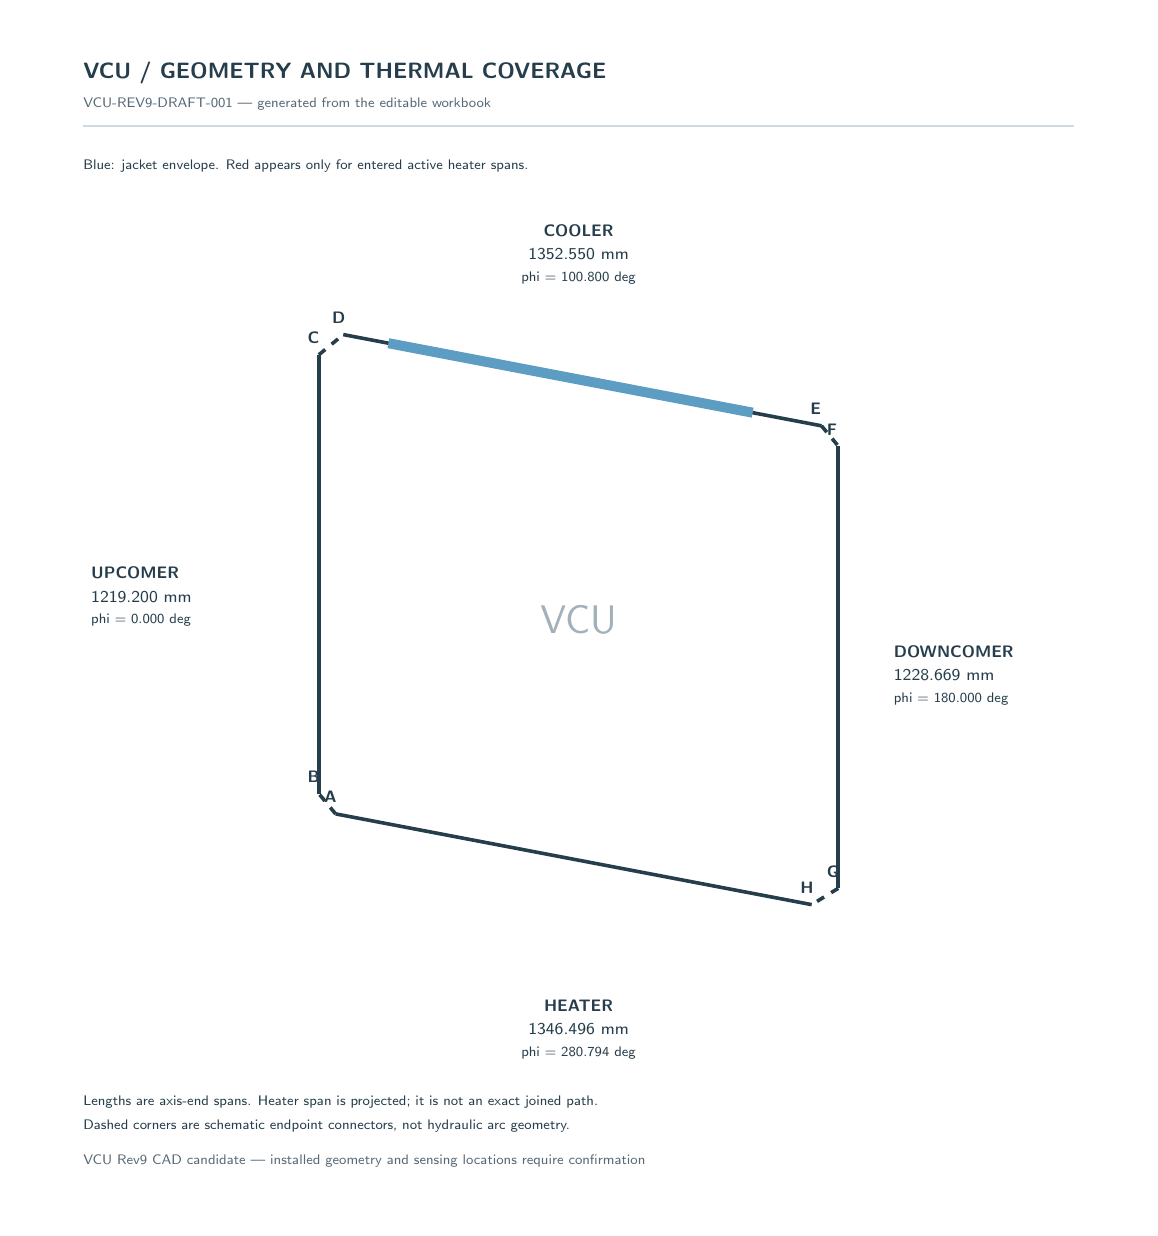
\begin{tikzpicture}[x=0.01cm,y=-0.01cm]
\path[use as bounding box] (0,0) rectangle (1400,1500);
\definecolor{c263D4B}{HTML}{263D4B}
\definecolor{c576976}{HTML}{576976}
\definecolor{c5D9DC3}{HTML}{5D9DC3}
\definecolor{cA3B0B9}{HTML}{A3B0B9}
\definecolor{cCFD9DF}{HTML}{CFD9DF}
\node[anchor=base west,inner sep=0pt,text=c263D4B,font=\sffamily\fontsize{8.40}{10.20}\selectfont\bfseries] at (70.000,65.000) {VCU / GEOMETRY AND THERMAL COVERAGE};
\node[anchor=base west,inner sep=0pt,text=c576976,font=\sffamily\fontsize{4.76}{5.78}\selectfont] at (70.000,102.000) {VCU-REV9-DRAFT-001 | generated from the editable workbook};
\draw[draw=cCFD9DF,line width=0.520pt] (70.000,125.000) -- (1330.000,125.000);
\draw[draw=c263D4B,line width=1.300pt] (370.000,973.358) -- (370.000,415.678);
\draw[draw=c263D4B,line width=1.300pt,dashed] (370.000,415.678) -- (401.040,390.000);
\draw[draw=c263D4B,line width=1.300pt] (401.040,390.000) -- (1008.757,505.928);
\draw[draw=c263D4B,line width=1.300pt,dashed] (1008.757,505.928) -- (1030.000,531.607);
\draw[draw=c263D4B,line width=1.300pt] (1030.000,531.607) -- (1030.000,1093.617);
\draw[draw=c263D4B,line width=1.300pt,dashed] (1030.000,1093.617) -- (996.253,1114.378);
\draw[draw=c263D4B,line width=1.300pt] (996.253,1114.378) -- (391.243,999.036);
\draw[draw=c263D4B,line width=1.300pt,dashed] (391.243,999.036) -- (370.000,973.358);
\draw[draw=c5D9DC3,line width=3.640pt] (458.355,400.933) -- (921.276,489.240);
\node[anchor=base west,inner sep=0pt,text=c263D4B,font=\sffamily\fontsize{5.60}{6.80}\selectfont\bfseries] at (355.000,959.358) {B};
\node[anchor=base west,inner sep=0pt,text=c263D4B,font=\sffamily\fontsize{5.60}{6.80}\selectfont\bfseries] at (355.000,401.678) {C};
\node[anchor=base west,inner sep=0pt,text=c263D4B,font=\sffamily\fontsize{5.60}{6.80}\selectfont\bfseries] at (386.040,376.000) {D};
\node[anchor=base west,inner sep=0pt,text=c263D4B,font=\sffamily\fontsize{5.60}{6.80}\selectfont\bfseries] at (993.757,491.928) {E};
\node[anchor=base west,inner sep=0pt,text=c263D4B,font=\sffamily\fontsize{5.60}{6.80}\selectfont\bfseries] at (1015.000,517.607) {F};
\node[anchor=base west,inner sep=0pt,text=c263D4B,font=\sffamily\fontsize{5.60}{6.80}\selectfont\bfseries] at (1015.000,1079.617) {G};
\node[anchor=base west,inner sep=0pt,text=c263D4B,font=\sffamily\fontsize{5.60}{6.80}\selectfont\bfseries] at (981.253,1100.378) {H};
\node[anchor=base west,inner sep=0pt,text=c263D4B,font=\sffamily\fontsize{5.60}{6.80}\selectfont\bfseries] at (376.243,985.036) {A};
\node[anchor=base,inner sep=0pt,text=cA3B0B9,font=\sffamily\fontsize{15.12}{18.36}\selectfont] at (700.000,770.000) {VCU};
\node[anchor=base west,inner sep=0pt,text=c263D4B,font=\sffamily\fontsize{6.16}{7.48}\selectfont\bfseries] at (80.000,700.000) {UPCOMER};
\node[anchor=base west,inner sep=0pt,text=c263D4B,font=\sffamily\fontsize{5.60}{6.80}\selectfont] at (80.000,730.000) {1219.200 mm};
\node[anchor=base west,inner sep=0pt,text=c263D4B,font=\sffamily\fontsize{4.76}{5.78}\selectfont] at (80.000,757.000) {phi = 0.000 deg};
\node[anchor=base,inner sep=0pt,text=c263D4B,font=\sffamily\fontsize{6.16}{7.48}\selectfont\bfseries] at (700.000,265.000) {COOLER};
\node[anchor=base,inner sep=0pt,text=c263D4B,font=\sffamily\fontsize{5.60}{6.80}\selectfont] at (700.000,295.000) {1352.550 mm};
\node[anchor=base,inner sep=0pt,text=c263D4B,font=\sffamily\fontsize{4.76}{5.78}\selectfont] at (700.000,322.000) {phi = 100.800 deg};
\node[anchor=base west,inner sep=0pt,text=c263D4B,font=\sffamily\fontsize{6.16}{7.48}\selectfont\bfseries] at (1100.000,800.000) {DOWNCOMER};
\node[anchor=base west,inner sep=0pt,text=c263D4B,font=\sffamily\fontsize{5.60}{6.80}\selectfont] at (1100.000,830.000) {1228.669 mm};
\node[anchor=base west,inner sep=0pt,text=c263D4B,font=\sffamily\fontsize{4.76}{5.78}\selectfont] at (1100.000,857.000) {phi = 180.000 deg};
\node[anchor=base,inner sep=0pt,text=c263D4B,font=\sffamily\fontsize{6.16}{7.48}\selectfont\bfseries] at (700.000,1250.000) {HEATER};
\node[anchor=base,inner sep=0pt,text=c263D4B,font=\sffamily\fontsize{5.60}{6.80}\selectfont] at (700.000,1280.000) {1346.496 mm};
\node[anchor=base,inner sep=0pt,text=c263D4B,font=\sffamily\fontsize{4.76}{5.78}\selectfont] at (700.000,1307.000) {phi = 280.794 deg};
\node[anchor=base west,inner sep=0pt,text=c263D4B,font=\sffamily\fontsize{5.04}{6.12}\selectfont] at (70.000,180.000) {Blue: jacket envelope. Red appears only for entered active heater spans.};
\node[anchor=base west,inner sep=0pt,text=c263D4B,font=\sffamily\fontsize{4.76}{5.78}\selectfont] at (70.000,1370.000) {Lengths are axis-end spans. Heater span is projected; it is not an exact joined path.};
\node[anchor=base west,inner sep=0pt,text=c263D4B,font=\sffamily\fontsize{4.76}{5.78}\selectfont] at (70.000,1400.000) {Dashed corners are schematic endpoint connectors, not hydraulic arc geometry.};
\node[anchor=base west,inner sep=0pt,text=c576976,font=\sffamily\fontsize{4.48}{5.44}\selectfont] at (70.000,1445.000) {VCU Rev9 CAD candidate | installed geometry and sensing locations require confirmation};
\end{tikzpicture}
}\end{center}
\clearpage\thispagestyle{empty}
\begin{center}\resizebox{\textwidth}{!}{%
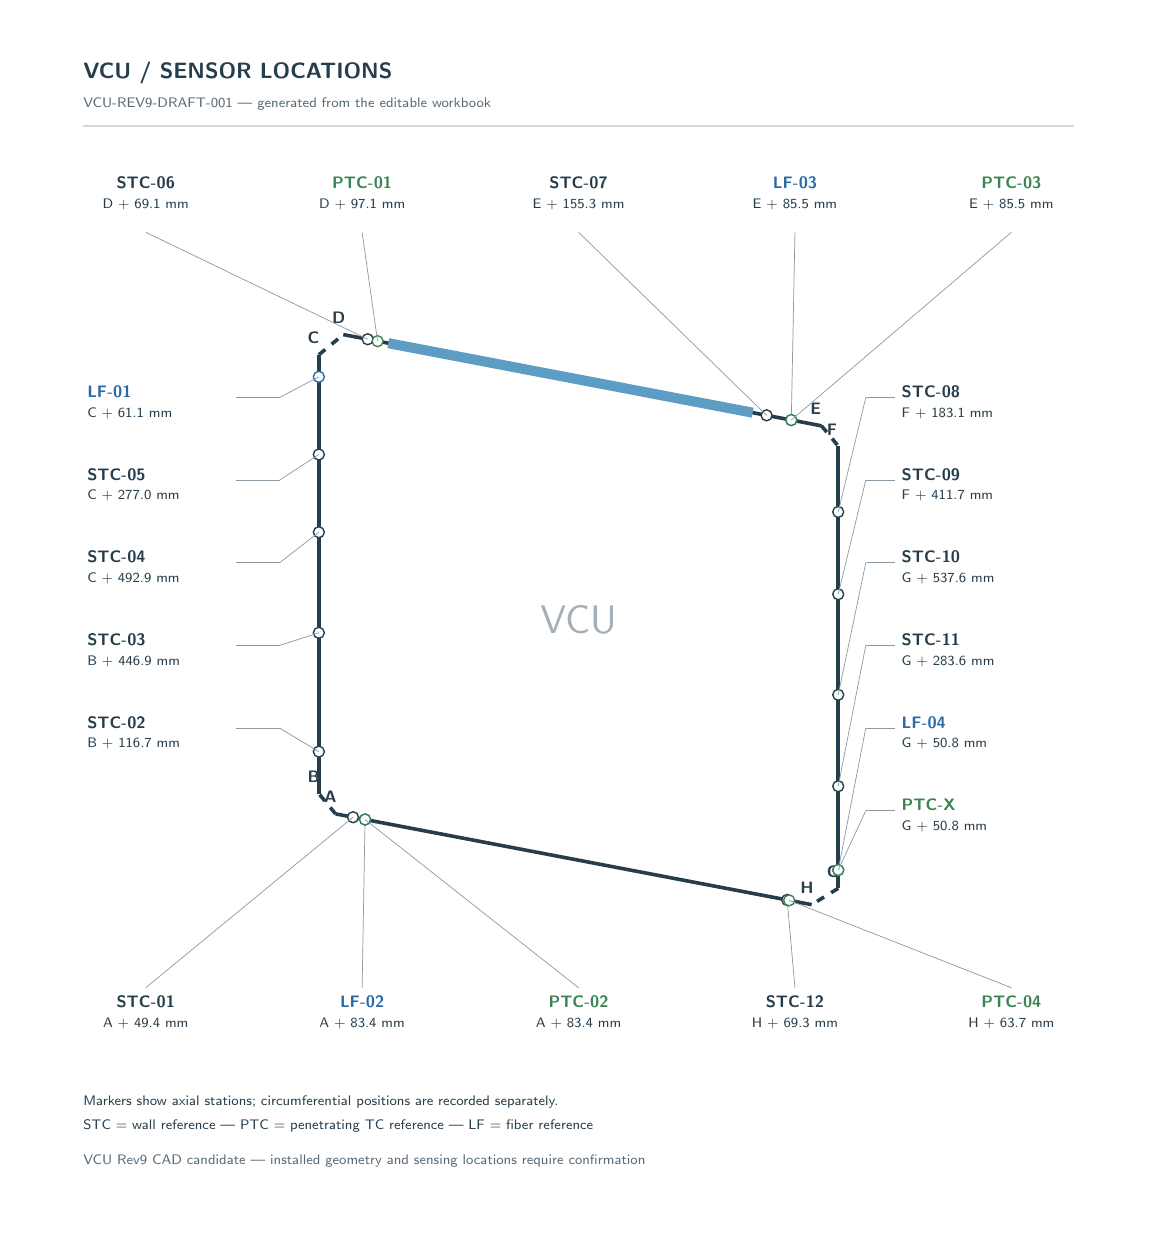
\begin{tikzpicture}[x=0.01cm,y=-0.01cm]
\path[use as bounding box] (0,0) rectangle (1400,1500);
\definecolor{c263D4B}{HTML}{263D4B}
\definecolor{c286AA6}{HTML}{286AA6}
\definecolor{c388452}{HTML}{388452}
\definecolor{c576976}{HTML}{576976}
\definecolor{c5D9DC3}{HTML}{5D9DC3}
\definecolor{c8B9AA5}{HTML}{8B9AA5}
\definecolor{cA3B0B9}{HTML}{A3B0B9}
\definecolor{cCFD9DF}{HTML}{CFD9DF}
\node[anchor=base west,inner sep=0pt,text=c263D4B,font=\sffamily\fontsize{8.40}{10.20}\selectfont\bfseries] at (70.000,65.000) {VCU / SENSOR LOCATIONS};
\node[anchor=base west,inner sep=0pt,text=c576976,font=\sffamily\fontsize{4.76}{5.78}\selectfont] at (70.000,102.000) {VCU-REV9-DRAFT-001 | generated from the editable workbook};
\draw[draw=cCFD9DF,line width=0.520pt] (70.000,125.000) -- (1330.000,125.000);
\draw[draw=c263D4B,line width=1.300pt] (370.000,973.358) -- (370.000,415.678);
\draw[draw=c263D4B,line width=1.300pt,dashed] (370.000,415.678) -- (401.040,390.000);
\draw[draw=c263D4B,line width=1.300pt] (401.040,390.000) -- (1008.757,505.928);
\draw[draw=c263D4B,line width=1.300pt,dashed] (1008.757,505.928) -- (1030.000,531.607);
\draw[draw=c263D4B,line width=1.300pt] (1030.000,531.607) -- (1030.000,1093.617);
\draw[draw=c263D4B,line width=1.300pt,dashed] (1030.000,1093.617) -- (996.253,1114.378);
\draw[draw=c263D4B,line width=1.300pt] (996.253,1114.378) -- (391.243,999.036);
\draw[draw=c263D4B,line width=1.300pt,dashed] (391.243,999.036) -- (370.000,973.358);
\draw[draw=c5D9DC3,line width=3.640pt] (458.355,400.933) -- (921.276,489.240);
\node[anchor=base west,inner sep=0pt,text=c263D4B,font=\sffamily\fontsize{5.60}{6.80}\selectfont\bfseries] at (355.000,959.358) {B};
\node[anchor=base west,inner sep=0pt,text=c263D4B,font=\sffamily\fontsize{5.60}{6.80}\selectfont\bfseries] at (355.000,401.678) {C};
\node[anchor=base west,inner sep=0pt,text=c263D4B,font=\sffamily\fontsize{5.60}{6.80}\selectfont\bfseries] at (386.040,376.000) {D};
\node[anchor=base west,inner sep=0pt,text=c263D4B,font=\sffamily\fontsize{5.60}{6.80}\selectfont\bfseries] at (993.757,491.928) {E};
\node[anchor=base west,inner sep=0pt,text=c263D4B,font=\sffamily\fontsize{5.60}{6.80}\selectfont\bfseries] at (1015.000,517.607) {F};
\node[anchor=base west,inner sep=0pt,text=c263D4B,font=\sffamily\fontsize{5.60}{6.80}\selectfont\bfseries] at (1015.000,1079.617) {G};
\node[anchor=base west,inner sep=0pt,text=c263D4B,font=\sffamily\fontsize{5.60}{6.80}\selectfont\bfseries] at (981.253,1100.378) {H};
\node[anchor=base west,inner sep=0pt,text=c263D4B,font=\sffamily\fontsize{5.60}{6.80}\selectfont\bfseries] at (376.243,985.036) {A};
\node[anchor=base,inner sep=0pt,text=cA3B0B9,font=\sffamily\fontsize{15.12}{18.36}\selectfont] at (700.000,770.000) {VCU};
\draw[fill=white,draw=c286AA6,line width=0.5pt] (370.000,443.633) circle (7);
\draw[draw=c8B9AA5,line width=0.260pt] (370.000,443.633) -- (320.000,470.000);
\draw[draw=c8B9AA5,line width=0.260pt] (320.000,470.000) -- (265.000,470.000);
\node[anchor=base west,inner sep=0pt,text=c286AA6,font=\sffamily\fontsize{5.60}{6.80}\selectfont\bfseries] at (75.000,470.000) {LF-01};
\node[anchor=base west,inner sep=0pt,text=c263D4B,font=\sffamily\fontsize{4.48}{5.44}\selectfont] at (75.000,495.000) {C + 61.1 mm};
\draw[fill=white,draw=c263D4B,line width=0.5pt] (370.000,542.388) circle (7);
\draw[draw=c8B9AA5,line width=0.260pt] (370.000,542.388) -- (320.000,575.000);
\draw[draw=c8B9AA5,line width=0.260pt] (320.000,575.000) -- (265.000,575.000);
\node[anchor=base west,inner sep=0pt,text=c263D4B,font=\sffamily\fontsize{5.60}{6.80}\selectfont\bfseries] at (75.000,575.000) {STC-05};
\node[anchor=base west,inner sep=0pt,text=c263D4B,font=\sffamily\fontsize{4.48}{5.44}\selectfont] at (75.000,600.000) {C + 277.0 mm};
\draw[fill=white,draw=c263D4B,line width=0.5pt] (370.000,641.144) circle (7);
\draw[draw=c8B9AA5,line width=0.260pt] (370.000,641.144) -- (320.000,680.000);
\draw[draw=c8B9AA5,line width=0.260pt] (320.000,680.000) -- (265.000,680.000);
\node[anchor=base west,inner sep=0pt,text=c263D4B,font=\sffamily\fontsize{5.60}{6.80}\selectfont\bfseries] at (75.000,680.000) {STC-04};
\node[anchor=base west,inner sep=0pt,text=c263D4B,font=\sffamily\fontsize{4.48}{5.44}\selectfont] at (75.000,705.000) {C + 492.9 mm};
\draw[fill=white,draw=c263D4B,line width=0.5pt] (370.000,768.946) circle (7);
\draw[draw=c8B9AA5,line width=0.260pt] (370.000,768.946) -- (320.000,785.000);
\draw[draw=c8B9AA5,line width=0.260pt] (320.000,785.000) -- (265.000,785.000);
\node[anchor=base west,inner sep=0pt,text=c263D4B,font=\sffamily\fontsize{5.60}{6.80}\selectfont\bfseries] at (75.000,785.000) {STC-03};
\node[anchor=base west,inner sep=0pt,text=c263D4B,font=\sffamily\fontsize{4.48}{5.44}\selectfont] at (75.000,810.000) {B + 446.9 mm};
\draw[fill=white,draw=c263D4B,line width=0.5pt] (370.000,919.984) circle (7);
\draw[draw=c8B9AA5,line width=0.260pt] (370.000,919.984) -- (320.000,890.000);
\draw[draw=c8B9AA5,line width=0.260pt] (320.000,890.000) -- (265.000,890.000);
\node[anchor=base west,inner sep=0pt,text=c263D4B,font=\sffamily\fontsize{5.60}{6.80}\selectfont\bfseries] at (75.000,890.000) {STC-02};
\node[anchor=base west,inner sep=0pt,text=c263D4B,font=\sffamily\fontsize{4.48}{5.44}\selectfont] at (75.000,915.000) {B + 116.7 mm};
\draw[fill=white,draw=c263D4B,line width=0.5pt] (432.106,395.926) circle (7);
\draw[draw=c8B9AA5,line width=0.260pt] (432.106,395.926) -- (150.000,260.000);
\node[anchor=base,inner sep=0pt,text=c263D4B,font=\sffamily\fontsize{5.60}{6.80}\selectfont\bfseries] at (150.000,205.000) {STC-06};
\node[anchor=base,inner sep=0pt,text=c263D4B,font=\sffamily\fontsize{4.48}{5.44}\selectfont] at (150.000,230.000) {D + 69.1 mm};
\draw[fill=white,draw=c388452,line width=0.5pt] (444.659,398.321) circle (7);
\draw[draw=c8B9AA5,line width=0.260pt] (444.659,398.321) -- (425.000,260.000);
\node[anchor=base,inner sep=0pt,text=c388452,font=\sffamily\fontsize{5.60}{6.80}\selectfont\bfseries] at (425.000,205.000) {PTC-01};
\node[anchor=base,inner sep=0pt,text=c263D4B,font=\sffamily\fontsize{4.48}{5.44}\selectfont] at (425.000,230.000) {D + 97.1 mm};
\draw[fill=white,draw=c263D4B,line width=0.5pt] (938.965,492.615) circle (7);
\draw[draw=c8B9AA5,line width=0.260pt] (938.965,492.615) -- (700.000,260.000);
\node[anchor=base,inner sep=0pt,text=c263D4B,font=\sffamily\fontsize{5.60}{6.80}\selectfont\bfseries] at (700.000,205.000) {STC-07};
\node[anchor=base,inner sep=0pt,text=c263D4B,font=\sffamily\fontsize{4.48}{5.44}\selectfont] at (700.000,230.000) {E + 155.3 mm};
\draw[fill=white,draw=c286AA6,line width=0.5pt] (970.350,498.602) circle (7);
\draw[draw=c8B9AA5,line width=0.260pt] (970.350,498.602) -- (975.000,260.000);
\node[anchor=base,inner sep=0pt,text=c286AA6,font=\sffamily\fontsize{5.60}{6.80}\selectfont\bfseries] at (975.000,205.000) {LF-03};
\node[anchor=base,inner sep=0pt,text=c263D4B,font=\sffamily\fontsize{4.48}{5.44}\selectfont] at (975.000,230.000) {E + 85.5 mm};
\draw[fill=white,draw=c388452,line width=0.5pt] (970.350,498.602) circle (7);
\draw[draw=c8B9AA5,line width=0.260pt] (970.350,498.602) -- (1250.000,260.000);
\node[anchor=base,inner sep=0pt,text=c388452,font=\sffamily\fontsize{5.60}{6.80}\selectfont\bfseries] at (1250.000,205.000) {PTC-03};
\node[anchor=base,inner sep=0pt,text=c263D4B,font=\sffamily\fontsize{4.48}{5.44}\selectfont] at (1250.000,230.000) {E + 85.5 mm};
\draw[fill=white,draw=c263D4B,line width=0.5pt] (1030.000,615.361) circle (7);
\draw[draw=c8B9AA5,line width=0.260pt] (1030.000,615.361) -- (1065.000,470.000);
\draw[draw=c8B9AA5,line width=0.260pt] (1065.000,470.000) -- (1102.000,470.000);
\node[anchor=base west,inner sep=0pt,text=c263D4B,font=\sffamily\fontsize{5.60}{6.80}\selectfont\bfseries] at (1110.000,470.000) {STC-08};
\node[anchor=base west,inner sep=0pt,text=c263D4B,font=\sffamily\fontsize{4.48}{5.44}\selectfont] at (1110.000,495.000) {F + 183.1 mm};
\draw[fill=white,draw=c263D4B,line width=0.5pt] (1030.000,719.926) circle (7);
\draw[draw=c8B9AA5,line width=0.260pt] (1030.000,719.926) -- (1065.000,575.000);
\draw[draw=c8B9AA5,line width=0.260pt] (1065.000,575.000) -- (1102.000,575.000);
\node[anchor=base west,inner sep=0pt,text=c263D4B,font=\sffamily\fontsize{5.60}{6.80}\selectfont\bfseries] at (1110.000,575.000) {STC-09};
\node[anchor=base west,inner sep=0pt,text=c263D4B,font=\sffamily\fontsize{4.48}{5.44}\selectfont] at (1110.000,600.000) {F + 411.7 mm};
\draw[fill=white,draw=c263D4B,line width=0.5pt] (1030.000,847.728) circle (7);
\draw[draw=c8B9AA5,line width=0.260pt] (1030.000,847.728) -- (1065.000,680.000);
\draw[draw=c8B9AA5,line width=0.260pt] (1065.000,680.000) -- (1102.000,680.000);
\node[anchor=base west,inner sep=0pt,text=c263D4B,font=\sffamily\fontsize{5.60}{6.80}\selectfont\bfseries] at (1110.000,680.000) {STC-10};
\node[anchor=base west,inner sep=0pt,text=c263D4B,font=\sffamily\fontsize{4.48}{5.44}\selectfont] at (1110.000,705.000) {G + 537.6 mm};
\draw[fill=white,draw=c263D4B,line width=0.5pt] (1030.000,963.911) circle (7);
\draw[draw=c8B9AA5,line width=0.260pt] (1030.000,963.911) -- (1065.000,785.000);
\draw[draw=c8B9AA5,line width=0.260pt] (1065.000,785.000) -- (1102.000,785.000);
\node[anchor=base west,inner sep=0pt,text=c263D4B,font=\sffamily\fontsize{5.60}{6.80}\selectfont\bfseries] at (1110.000,785.000) {STC-11};
\node[anchor=base west,inner sep=0pt,text=c263D4B,font=\sffamily\fontsize{4.48}{5.44}\selectfont] at (1110.000,810.000) {G + 283.6 mm};
\draw[fill=white,draw=c286AA6,line width=0.5pt] (1030.000,1070.381) circle (7);
\draw[draw=c8B9AA5,line width=0.260pt] (1030.000,1070.381) -- (1065.000,890.000);
\draw[draw=c8B9AA5,line width=0.260pt] (1065.000,890.000) -- (1102.000,890.000);
\node[anchor=base west,inner sep=0pt,text=c286AA6,font=\sffamily\fontsize{5.60}{6.80}\selectfont\bfseries] at (1110.000,890.000) {LF-04};
\node[anchor=base west,inner sep=0pt,text=c263D4B,font=\sffamily\fontsize{4.48}{5.44}\selectfont] at (1110.000,915.000) {G + 50.8 mm};
\draw[fill=white,draw=c388452,line width=0.5pt] (1030.000,1070.381) circle (7);
\draw[draw=c8B9AA5,line width=0.260pt] (1030.000,1070.381) -- (1065.000,995.000);
\draw[draw=c8B9AA5,line width=0.260pt] (1065.000,995.000) -- (1102.000,995.000);
\node[anchor=base west,inner sep=0pt,text=c388452,font=\sffamily\fontsize{5.60}{6.80}\selectfont\bfseries] at (1110.000,995.000) {PTC-X};
\node[anchor=base west,inner sep=0pt,text=c263D4B,font=\sffamily\fontsize{4.48}{5.44}\selectfont] at (1110.000,1020.000) {G + 50.8 mm};
\draw[fill=white,draw=c263D4B,line width=0.5pt] (413.452,1003.270) circle (7);
\draw[draw=c8B9AA5,line width=0.260pt] (413.452,1003.270) -- (150.000,1220.000);
\node[anchor=base,inner sep=0pt,text=c263D4B,font=\sffamily\fontsize{5.60}{6.80}\selectfont\bfseries] at (150.000,1245.000) {STC-01};
\node[anchor=base,inner sep=0pt,text=c263D4B,font=\sffamily\fontsize{4.48}{5.44}\selectfont] at (150.000,1270.000) {A + 49.4 mm};
\draw[fill=white,draw=c286AA6,line width=0.5pt] (428.714,1006.180) circle (7);
\draw[draw=c8B9AA5,line width=0.260pt] (428.714,1006.180) -- (425.000,1220.000);
\node[anchor=base,inner sep=0pt,text=c286AA6,font=\sffamily\fontsize{5.60}{6.80}\selectfont\bfseries] at (425.000,1245.000) {LF-02};
\node[anchor=base,inner sep=0pt,text=c263D4B,font=\sffamily\fontsize{4.48}{5.44}\selectfont] at (425.000,1270.000) {A + 83.4 mm};
\draw[fill=white,draw=c388452,line width=0.5pt] (428.714,1006.180) circle (7);
\draw[draw=c8B9AA5,line width=0.260pt] (428.714,1006.180) -- (700.000,1220.000);
\node[anchor=base,inner sep=0pt,text=c388452,font=\sffamily\fontsize{5.60}{6.80}\selectfont\bfseries] at (700.000,1245.000) {PTC-02};
\node[anchor=base,inner sep=0pt,text=c263D4B,font=\sffamily\fontsize{4.48}{5.44}\selectfont] at (700.000,1270.000) {A + 83.4 mm};
\draw[fill=white,draw=c263D4B,line width=0.5pt] (965.118,1108.442) circle (7);
\draw[draw=c8B9AA5,line width=0.260pt] (965.118,1108.442) -- (975.000,1220.000);
\node[anchor=base,inner sep=0pt,text=c263D4B,font=\sffamily\fontsize{5.60}{6.80}\selectfont\bfseries] at (975.000,1245.000) {STC-12};
\node[anchor=base,inner sep=0pt,text=c263D4B,font=\sffamily\fontsize{4.48}{5.44}\selectfont] at (975.000,1270.000) {H + 69.3 mm};
\draw[fill=white,draw=c388452,line width=0.5pt] (967.624,1108.920) circle (7);
\draw[draw=c8B9AA5,line width=0.260pt] (967.624,1108.920) -- (1250.000,1220.000);
\node[anchor=base,inner sep=0pt,text=c388452,font=\sffamily\fontsize{5.60}{6.80}\selectfont\bfseries] at (1250.000,1245.000) {PTC-04};
\node[anchor=base,inner sep=0pt,text=c263D4B,font=\sffamily\fontsize{4.48}{5.44}\selectfont] at (1250.000,1270.000) {H + 63.7 mm};
\node[anchor=base west,inner sep=0pt,text=c263D4B,font=\sffamily\fontsize{4.76}{5.78}\selectfont] at (70.000,1370.000) {Markers show axial stations; circumferential positions are recorded separately.};
\node[anchor=base west,inner sep=0pt,text=c263D4B,font=\sffamily\fontsize{4.76}{5.78}\selectfont] at (70.000,1400.000) {STC = wall reference | PTC = penetrating TC reference | LF = fiber reference};
\node[anchor=base west,inner sep=0pt,text=c576976,font=\sffamily\fontsize{4.48}{5.44}\selectfont] at (70.000,1445.000) {VCU Rev9 CAD candidate | installed geometry and sensing locations require confirmation};
\end{tikzpicture}
}\end{center}
\clearpage\thispagestyle{empty}
\begin{center}\resizebox{\textwidth}{!}{%
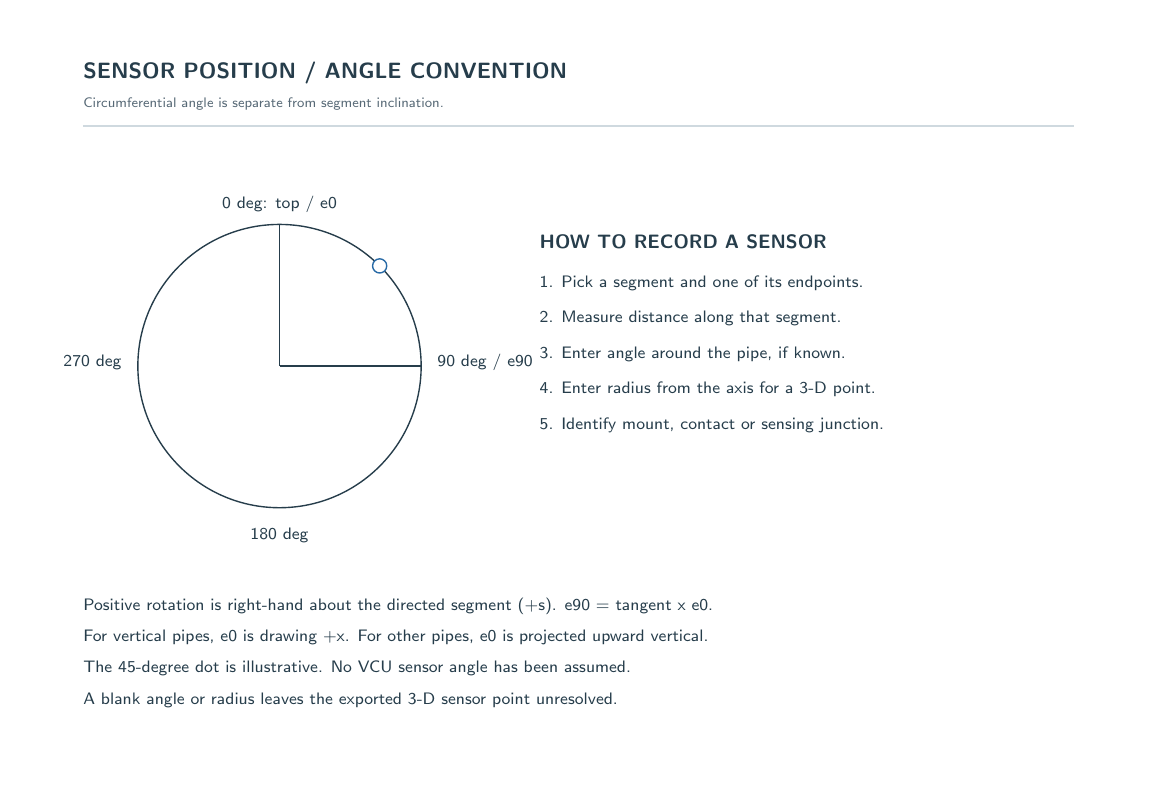
\begin{tikzpicture}[x=0.01cm,y=-0.01cm]
\path[use as bounding box] (0,0) rectangle (1400,950);
\definecolor{c263D4B}{HTML}{263D4B}
\definecolor{c286AA6}{HTML}{286AA6}
\definecolor{c576976}{HTML}{576976}
\definecolor{cCFD9DF}{HTML}{CFD9DF}
\node[anchor=base west,inner sep=0pt,text=c263D4B,font=\sffamily\fontsize{8.40}{10.20}\selectfont\bfseries] at (70.000,65.000) {SENSOR POSITION / ANGLE CONVENTION};
\node[anchor=base west,inner sep=0pt,text=c576976,font=\sffamily\fontsize{4.76}{5.78}\selectfont] at (70.000,102.000) {Circumferential angle is separate from segment inclination.};
\draw[draw=cCFD9DF,line width=0.520pt] (70.000,125.000) -- (1330.000,125.000);
\draw[fill=white,draw=c263D4B,line width=0.5pt] (320.000,430.000) circle (180);
\draw[draw=c263D4B,line width=0.520pt] (320.000,430.000) -- (320.000,250.000);
\draw[draw=c263D4B,line width=0.520pt] (320.000,430.000) -- (500.000,430.000);
\node[anchor=base,inner sep=0pt,text=c263D4B,font=\sffamily\fontsize{5.88}{7.14}\selectfont] at (320.000,230.000) {0 deg: top / e0};
\node[anchor=base west,inner sep=0pt,text=c263D4B,font=\sffamily\fontsize{5.88}{7.14}\selectfont] at (520.000,430.000) {90 deg / e90};
\node[anchor=base,inner sep=0pt,text=c263D4B,font=\sffamily\fontsize{5.88}{7.14}\selectfont] at (320.000,650.000) {180 deg};
\node[anchor=base east,inner sep=0pt,text=c263D4B,font=\sffamily\fontsize{5.88}{7.14}\selectfont] at (120.000,430.000) {270 deg};
\draw[fill=white,draw=c286AA6,line width=0.5pt] (447.279,302.721) circle (9);
\node[anchor=base west,inner sep=0pt,text=c263D4B,font=\sffamily\fontsize{6.72}{8.16}\selectfont\bfseries] at (650.000,280.000) {HOW TO RECORD A SENSOR};
\node[anchor=base west,inner sep=0pt,text=c263D4B,font=\sffamily\fontsize{5.60}{6.80}\selectfont] at (650.000,330.000) {1. Pick a segment and one of its endpoints.};
\node[anchor=base west,inner sep=0pt,text=c263D4B,font=\sffamily\fontsize{5.60}{6.80}\selectfont] at (650.000,375.000) {2. Measure distance along that segment.};
\node[anchor=base west,inner sep=0pt,text=c263D4B,font=\sffamily\fontsize{5.60}{6.80}\selectfont] at (650.000,420.000) {3. Enter angle around the pipe, if known.};
\node[anchor=base west,inner sep=0pt,text=c263D4B,font=\sffamily\fontsize{5.60}{6.80}\selectfont] at (650.000,465.000) {4. Enter radius from the axis for a 3-D point.};
\node[anchor=base west,inner sep=0pt,text=c263D4B,font=\sffamily\fontsize{5.60}{6.80}\selectfont] at (650.000,510.000) {5. Identify mount, contact or sensing junction.};
\node[anchor=base west,inner sep=0pt,text=c263D4B,font=\sffamily\fontsize{5.60}{6.80}\selectfont] at (70.000,740.000) {Positive rotation is right-hand about the directed segment (+s). e90 = tangent x e0.};
\node[anchor=base west,inner sep=0pt,text=c263D4B,font=\sffamily\fontsize{5.60}{6.80}\selectfont] at (70.000,780.000) {For vertical pipes, e0 is drawing +x. For other pipes, e0 is projected upward vertical.};
\node[anchor=base west,inner sep=0pt,text=c263D4B,font=\sffamily\fontsize{5.60}{6.80}\selectfont] at (70.000,820.000) {The 45-degree dot is illustrative. No VCU sensor angle has been assumed.};
\node[anchor=base west,inner sep=0pt,text=c263D4B,font=\sffamily\fontsize{5.60}{6.80}\selectfont] at (70.000,860.000) {A blank angle or radius leaves the exported 3-D sensor point unresolved.};
\end{tikzpicture}
}\end{center}
\clearpage\section{Current candidate input tables}
\subsection*{Main-loop geometry}
\small\setlength{\tabcolsep}{4pt}
\begin{longtable}{p{0.23\textwidth}p{0.12\textwidth}p{0.16\textwidth}p{0.14\textwidth}p{0.22\textwidth}}
\toprule
\textbf{Segment} & \textbf{Endpoints} & \textbf{Length mm} & \textbf{Phi deg} & \textbf{Evidence} \\\midrule\endhead
upcomer & B to C & 1219.200 & 0.000 & CAD-derived \\[3pt]
upper\_left\_bend & C to D & \textit{Unknown} & \textit{Unknown} & CAD-derived \\[3pt]
cooler & D to E & 1352.550 & 100.800 & CAD-derived \\[3pt]
upper\_right\_bend & E to F & \textit{Unknown} & \textit{Unknown} & CAD-derived \\[3pt]
downcomer & F to G & 1228.669 & 180.000 & CAD-derived \\[3pt]
lower\_right\_bend & G to H & \textit{Unknown} & \textit{Unknown} & CAD-derived \\[3pt]
heater & H to A & 1346.496 & 280.794 & CAD-derived \\[3pt]
lower\_left\_bend & A to B & \textit{Unknown} & \textit{Unknown} & CAD-derived \\[3pt]
\bottomrule\end{longtable}\normalsize
Bends use offsets, not straight-length inputs. See the editable Geometry sheet and source length basis. The example forms do not populate these baseline cells.
\subsection*{Main-loop geometric sensor references}
\small\setlength{\tabcolsep}{4pt}
\begin{longtable}{p{0.17\textwidth}p{0.25\textwidth}p{0.1\textwidth}p{0.17\textwidth}p{0.17\textwidth}}
\toprule
\textbf{Sensor} & \textbf{Segment} & \textbf{From} & \textbf{Distance mm} & \textbf{Angle deg} \\\midrule\endhead
STC-02 & upcomer & B & 116.686 & \textit{Unknown} \\[3pt]
STC-03 & upcomer & B & 446.886 & \textit{Unknown} \\[3pt]
STC-04 & upcomer & C & 492.914 & \textit{Unknown} \\[3pt]
STC-05 & upcomer & C & 277.014 & \textit{Unknown} \\[3pt]
LF-01 & upcomer & C & 61.114 & \textit{Unknown} \\[3pt]
STC-06 & cooler & D & 69.142 & \textit{Unknown} \\[3pt]
PTC-01 & cooler & D & 97.080 & \textit{Unknown} \\[3pt]
STC-07 & cooler & E & 155.331 & \textit{Unknown} \\[3pt]
LF-03 & cooler & E & 85.481 & \textit{Unknown} \\[3pt]
PTC-03 & cooler & E & 85.481 & \textit{Unknown} \\[3pt]
STC-08 & downcomer & F & 183.105 & \textit{Unknown} \\[3pt]
STC-09 & downcomer & F & 411.705 & \textit{Unknown} \\[3pt]
STC-10 & downcomer & G & 537.564 & \textit{Unknown} \\[3pt]
STC-11 & downcomer & G & 283.564 & \textit{Unknown} \\[3pt]
LF-04 & downcomer & G & 50.800 & \textit{Unknown} \\[3pt]
PTC-X & downcomer & G & 50.800 & \textit{Unknown} \\[3pt]
PTC-04 & heater & H & 63.716 & \textit{Unknown} \\[3pt]
STC-12 & heater & H & 69.293 & \textit{Unknown} \\[3pt]
LF-02 & heater & A & 83.394 & \textit{Unknown} \\[3pt]
PTC-02 & heater & A & 83.394 & \textit{Unknown} \\[3pt]
STC-01 & heater & A & 49.428 & \textit{Unknown} \\[3pt]
\bottomrule\end{longtable}\normalsize
JTC-A/B are retained in Calibration, but jacket-port positions are not yet drawn. DAQ mappings, calibration and model mappings remain unknown unless separately entered with evidence.
\subsection*{VCU fluid choices}
Prop-30, air and water are permitted candidate options from the user. A circuit/run assignment is still required. The supplied draft phase campaign is Prop-30-specific.
\small\setlength{\tabcolsep}{4pt}
\begin{longtable}{p{0.15\textwidth}p{0.3\textwidth}p{0.22\textwidth}p{0.2\textwidth}}
\toprule
\textbf{Fluid} & \textbf{Product} & \textbf{Circuit} & \textbf{Range C} \\\midrule\endhead
PROP30 & Propylene glycol / water & \textit{Unknown} & \textit{Unknown} \\[3pt]
AIR & Air & \textit{Unknown} & \textit{Unknown} \\[3pt]
WATER & Water & \textit{Unknown} & \textit{Unknown} \\[3pt]
\bottomrule\end{longtable}\normalsize
\appendix
\clearpage\section{Complete requirements and evidence register}\label{requirements}
The Requirements workbook tab is the editable master. Each record states why the field is needed, who should supply it, where the requirement and evidence came from, what uses it supports, and what remains unresolved. Requirement provenance is distinct from evidence for a value.
\textbf{Review rule:} the records below describe candidate evidence. Approved choices require a recorded decision, scope and effective configuration; none has been established in this seed package.
\par\noindent\begin{minipage}{\textwidth}\small\setlength{\parskip}{2pt}
\subsection*{C01 | Facility and configuration ID}
\textbf{Purpose:} Tie measurements to one physical setup.\par
\textbf{Package / responsible team:} Configuration / Experimental team\par
\textbf{Applies to:} VCU; every configuration and affected run\par
\textbf{Requirement source / locator:} P0; Section 3 Method, document facility configuration\par
\textbf{Current evidence [Reported]:} VCU; prototype ID VCU-REV9-DRAFT-001\par
\textbf{Evidence source / locator:} USER / current workbook; Facility selection; Start sheet\par
\textbf{Review state:} Needs review\par
\textbf{Selected choice:} None selected\par
\textbf{Decision scope / rationale:} \textit{Unknown}\par
\textbf{Reviewer / date; effective configuration:} Pending; Unknown\par
\textbf{To resolve:} Which installed configuration and effective date does this identify?\par
\end{minipage}\par\vspace{5pt}
\par\noindent\begin{minipage}{\textwidth}\small\setlength{\parskip}{2pt}
\subsection*{C02 | Effective date and change history}
\textbf{Purpose:} Explain what changed between datasets.\par
\textbf{Package / responsible team:} Configuration / Experimental team\par
\textbf{Applies to:} VCU; every configuration and affected run\par
\textbf{Requirement source / locator:} P0; DESIGN; Campaign execution conventions; proposed revision log\par
\textbf{Current evidence [Unknown]:} Unknown\par
\textbf{Evidence source / locator:} None supplied; Not available\par
\textbf{Review state:} Needs information\par
\textbf{Selected choice:} None selected\par
\textbf{Decision scope / rationale:} \textit{Unknown}\par
\textbf{Reviewer / date; effective configuration:} Pending; Unknown\par
\textbf{To resolve:} Record effective date, author, changed item, reason, previous/new evidence, affected runs and whether recalibration or model revalidation is needed.\par
\end{minipage}\par\vspace{5pt}
\par\noindent\begin{minipage}{\textwidth}\small\setlength{\parskip}{2pt}
\subsection*{C03 | Reviewer, date and approved use}
\textbf{Purpose:} Record an actual release decision separately from evidence type.\par
\textbf{Package / responsible team:} Shared / Facility lead / package reviewer\par
\textbf{Applies to:} VCU; every configuration and affected run\par
\textbf{Requirement source / locator:} P0; Approval record and Section 3 Disposition\par
\textbf{Current evidence [Unknown]:} Unknown\par
\textbf{Evidence source / locator:} None supplied; Not available\par
\textbf{Review state:} Needs information\par
\textbf{Selected choice:} None selected\par
\textbf{Decision scope / rationale:} \textit{Unknown}\par
\textbf{Reviewer / date; effective configuration:} Pending; Unknown\par
\textbf{To resolve:} Who may release the package, and for which experiment/model use?\par
\end{minipage}\par\vspace{5pt}
\par\noindent\begin{minipage}{\textwidth}\small\setlength{\parskip}{2pt}
\subsection*{C04 | Source revision and file hash}
\textbf{Purpose:} Make the geometry baseline reproducible.\par
\textbf{Package / responsible team:} Shared / Experimental + computational\par
\textbf{Applies to:} VCU; 1-D and CFD / CHT\par
\textbf{Requirement source / locator:} R9; Sheet 8 source identity\par
\textbf{Current evidence [CAD-derived]:} Rev9 STEP SHA-256 78c6ae52bf39084f bd9b1306d28dcbe2 c1c4d5fccd334b0e 68c861022a1bfbcf\par
\textbf{Evidence source / locator:} R9; Sheet 8\par
\textbf{Review state:} Needs review\par
\textbf{Selected choice:} None selected\par
\textbf{Decision scope / rationale:} \textit{Unknown}\par
\textbf{Reviewer / date; effective configuration:} Pending; Unknown\par
\textbf{To resolve:} Does this source match installed VCU hardware?\par
\end{minipage}\par\vspace{5pt}
\par\noindent\begin{minipage}{\textwidth}\small\setlength{\parskip}{2pt}
\subsection*{C05 | Coordinate datum and axes}
\textbf{Purpose:} Give every location the same reference.\par
\textbf{Package / responsible team:} Configuration / Experimental + computational\par
\textbf{Applies to:} VCU; 1-D and CFD / CHT\par
\textbf{Requirement source / locator:} R9; Sheets 1 and 7\par
\textbf{Current evidence [CAD-derived]:} B origin; x right; y up; n normal; B-C-D-E-F-G-H-A-B\par
\textbf{Evidence source / locator:} R9; Sheets 1, 7\par
\textbf{Review state:} Needs review\par
\textbf{Selected choice:} None selected\par
\textbf{Decision scope / rationale:} \textit{Unknown}\par
\textbf{Reviewer / date; effective configuration:} Pending; Unknown\par
\textbf{To resolve:} Identify these points on a dated hardware photo.\par
\end{minipage}\par\vspace{5pt}
\par\noindent\begin{minipage}{\textwidth}\small\setlength{\parskip}{2pt}
\subsection*{C06 | Segment endpoints and straight length}
\textbf{Purpose:} Define the length being measured.\par
\textbf{Package / responsible team:} Configuration / Experimental team\par
\textbf{Applies to:} VCU; 1-D and CFD / CHT\par
\textbf{Requirement source / locator:} P0; SEG; Method geometry map; segment rows\par
\textbf{Current evidence [CAD-derived]:} Upcomer B-C 1219.200 mm; other spans in SEG\par
\textbf{Evidence source / locator:} SEG; upcomer row: reference\_\allowbreak{}length\_\allowbreak{}mm and length\_\allowbreak{}basis\par
\textbf{Review state:} Needs review\par
\textbf{Selected choice:} None selected\par
\textbf{Decision scope / rationale:} \textit{Unknown}\par
\textbf{Reviewer / date; effective configuration:} Pending; Unknown\par
\textbf{To resolve:} Measure axis-end span; do not substitute virtual-corner length.\par
\end{minipage}\par\vspace{5pt}
\par\noindent\begin{minipage}{\textwidth}\small\setlength{\parskip}{2pt}
\subsection*{C07 | Installed inclination and gravity direction}
\textbf{Purpose:} Determine elevation changes and buoyancy orientation.\par
\textbf{Package / responsible team:} Configuration / Experimental team\par
\textbf{Applies to:} VCU; 1-D and CFD / CHT\par
\textbf{Requirement source / locator:} P0; R9; Method geometry map; sheets 1-2\par
\textbf{Current evidence [CAD-derived]:} Inclined CAD cylinder axes 10.800 deg to horizontal\par
\textbf{Evidence source / locator:} R9; Sheets 1-2\par
\textbf{Review state:} Needs review\par
\textbf{Selected choice:} None selected\par
\textbf{Decision scope / rationale:} \textit{Unknown}\par
\textbf{Reviewer / date; effective configuration:} Pending; Unknown\par
\textbf{To resolve:} What is the measured installed tilt and uncertainty?\par
\end{minipage}\par\vspace{5pt}
\par\noindent\begin{minipage}{\textwidth}\small\setlength{\parskip}{2pt}
\subsection*{C08 | Bend geometry and length basis}
\textbf{Purpose:} Avoid replacing a chord with an arc.\par
\textbf{Package / responsible team:} Configuration / Experimental + computational\par
\textbf{Applies to:} VCU; 1-D and CFD / CHT\par
\textbf{Requirement source / locator:} SEG; Bend rows and length\_\allowbreak{}basis\par
\textbf{Current evidence [CAD-derived]:} Three torus arcs; G-H recovered spine qualified; exact joined path unresolved\par
\textbf{Evidence source / locator:} SEG; R9; Bend rows; sheet 2\par
\textbf{Review state:} Needs review\par
\textbf{Selected choice:} None selected\par
\textbf{Decision scope / rationale:} \textit{Unknown}\par
\textbf{Reviewer / date; effective configuration:} Pending; Unknown\par
\textbf{To resolve:} How will the physical bend be measured and represented?\par
\end{minipage}\par\vspace{5pt}
\par\noindent\begin{minipage}{\textwidth}\small\setlength{\parskip}{2pt}
\subsection*{C09 | Pipe inside diameter}
\textbf{Purpose:} Set fluid area, inventory and hydraulic dimension.\par
\textbf{Package / responsible team:} Configuration / Experimental team\par
\textbf{Applies to:} VCU; 1-D and CFD / CHT\par
\textbf{Requirement source / locator:} P0; DIA; Geometry map; Main swept loop\par
\textbf{Current evidence [Reported]:} Main CAD bore absent; notes report nominal 1.049 in (26.64 mm)\par
\textbf{Evidence source / locator:} DIA; MAT; Main swept loop row; VCU Piping lines 23-27\par
\textbf{Review state:} Needs review\par
\textbf{Selected choice:} None selected\par
\textbf{Decision scope / rationale:} \textit{Unknown}\par
\textbf{Reviewer / date; effective configuration:} Pending; Unknown\par
\textbf{To resolve:} Confirm actual bore/specification and local restrictions; keep CAD null.\par
\end{minipage}\par\vspace{5pt}
\par\noindent\begin{minipage}{\textwidth}\small\setlength{\parskip}{2pt}
\subsection*{C10 | Pipe outside diameter}
\textbf{Purpose:} Set wall and external thermal geometry.\par
\textbf{Package / responsible team:} Configuration / Experimental team\par
\textbf{Applies to:} VCU; 1-D and CFD / CHT\par
\textbf{Requirement source / locator:} DIA; Main swept loop row\par
\textbf{Current evidence [CAD-derived]:} 33.401 mm CAD OD\par
\textbf{Evidence source / locator:} DIA; Main swept loop / outer\_\allowbreak{}diameter\_\allowbreak{}mm\par
\textbf{Review state:} Needs review\par
\textbf{Selected choice:} None selected\par
\textbf{Decision scope / rationale:} \textit{Unknown}\par
\textbf{Reviewer / date; effective configuration:} Pending; Unknown\par
\textbf{To resolve:} Confirm installed OD and measurement uncertainty.\par
\end{minipage}\par\vspace{5pt}
\par\noindent\begin{minipage}{\textwidth}\small\setlength{\parskip}{2pt}
\subsection*{C11 | Pipe material grade and certificate}
\textbf{Purpose:} Identify the solid whose properties will be used.\par
\textbf{Package / responsible team:} Configuration / Experimental team\par
\textbf{Applies to:} VCU; 1-D and CFD / CHT\par
\textbf{Requirement source / locator:} P0; MAT; Geometry map; VCU Piping\par
\textbf{Current evidence [Reported]:} 316L, nominal 1-inch schedule 40 reported\par
\textbf{Evidence source / locator:} MAT; VCU Piping lines 23-27\par
\textbf{Review state:} Needs review\par
\textbf{Selected choice:} None selected\par
\textbf{Decision scope / rationale:} \textit{Unknown}\par
\textbf{Reviewer / date; effective configuration:} Pending; Unknown\par
\textbf{To resolve:} Provide purchase/specification or material certificate.\par
\end{minipage}\par\vspace{5pt}
\par\noindent\begin{minipage}{\textwidth}\small\setlength{\parskip}{2pt}
\subsection*{C12 | Dimension uncertainty and method}
\textbf{Purpose:} Propagate measurement uncertainty without using CAD print precision.\par
\textbf{Package / responsible team:} Configuration / Experimental team\par
\textbf{Applies to:} VCU; 1-D and CFD / CHT\par
\textbf{Requirement source / locator:} P0; DESIGN; Measurement uncertainties; proposed geometry uncertainty field\par
\textbf{Current evidence [Unknown]:} Unknown\par
\textbf{Evidence source / locator:} None supplied; Not available\par
\textbf{Review state:} Needs information\par
\textbf{Selected choice:} None selected\par
\textbf{Decision scope / rationale:} \textit{Unknown}\par
\textbf{Reviewer / date; effective configuration:} Pending; Unknown\par
\textbf{To resolve:} Record method, instrument, repeatability and uncertainty units for each dimension.\par
\end{minipage}\par\vspace{5pt}
\par\noindent\begin{minipage}{\textwidth}\small\setlength{\parskip}{2pt}
\subsection*{C13 | Insulation product and layer order}
\textbf{Purpose:} Identify the actual thermal stack.\par
\textbf{Package / responsible team:} Configuration / Experimental team\par
\textbf{Applies to:} VCU; 1-D and CFD / CHT\par
\textbf{Requirement source / locator:} P0; MAT; Geometry map; VCU insulation\par
\textbf{Current evidence [Reported]:} Main: fiberglass 5556K73; heater: calcium aluminum silicate 4057K14 reported\par
\textbf{Evidence source / locator:} MAT; Lines 29-44\par
\textbf{Review state:} Needs review\par
\textbf{Selected choice:} None selected\par
\textbf{Decision scope / rationale:} \textit{Unknown}\par
\textbf{Reviewer / date; effective configuration:} Pending; Unknown\par
\textbf{To resolve:} Which product and layers are installed on this exact segment?\par
\end{minipage}\par\vspace{5pt}
\par\noindent\begin{minipage}{\textwidth}\small\setlength{\parskip}{2pt}
\subsection*{C14 | Insulation thickness by section}
\textbf{Purpose:} Set the thermal resistance geometry.\par
\textbf{Package / responsible team:} Configuration / Experimental team\par
\textbf{Applies to:} VCU; 1-D and CFD / CHT\par
\textbf{Requirement source / locator:} P0; MAT; Geometry map; VCU insulation\par
\textbf{Current evidence [Reported]:} Most piping about 2 in; heater insulation 1/4 in reported\par
\textbf{Evidence source / locator:} MAT; Lines 29-44\par
\textbf{Review state:} Needs review\par
\textbf{Selected choice:} None selected\par
\textbf{Decision scope / rationale:} \textit{Unknown}\par
\textbf{Reviewer / date; effective configuration:} Pending; Unknown\par
\textbf{To resolve:} Measure each layer; do not apply either value everywhere.\par
\end{minipage}\par\vspace{5pt}
\par\noindent\begin{minipage}{\textwidth}\small\setlength{\parskip}{2pt}
\subsection*{C15 | Coverage start/end, gaps and condition}
\textbf{Purpose:} Capture uninsulated heat-loss paths.\par
\textbf{Package / responsible team:} Configuration / Experimental team\par
\textbf{Applies to:} VCU; 1-D and CFD / CHT\par
\textbf{Requirement source / locator:} P0; Method: facility and fluid configuration; geometry map\par
\textbf{Current evidence [Unknown]:} Unknown\par
\textbf{Evidence source / locator:} None supplied; Not available\par
\textbf{Review state:} Needs information\par
\textbf{Selected choice:} None selected\par
\textbf{Decision scope / rationale:} \textit{Unknown}\par
\textbf{Reviewer / date; effective configuration:} Pending; Unknown\par
\textbf{To resolve:} Supply evidence and request review.\par
\end{minipage}\par\vspace{5pt}
\par\noindent\begin{minipage}{\textwidth}\small\setlength{\parskip}{2pt}
\subsection*{C16 | Insulation contact and support details}
\textbf{Purpose:} Represent contact resistance and support heat paths.\par
\textbf{Package / responsible team:} Shared / Experimental + computational\par
\textbf{Applies to:} VCU; 1-D and CFD / CHT\par
\textbf{Requirement source / locator:} P0; HEAT; Geometry map; VCU Insulation\par
\textbf{Current evidence [Modeling assumption]:} Firm contact is explicitly an assumption in notes\par
\textbf{Evidence source / locator:} HEAT; VCU Insulation lines 7-10\par
\textbf{Review state:} Needs review\par
\textbf{Selected choice:} None selected\par
\textbf{Decision scope / rationale:} \textit{Unknown}\par
\textbf{Reviewer / date; effective configuration:} Pending; Unknown\par
\textbf{To resolve:} Is there evidence of contact, compression, gaps or support conduction?\par
\end{minipage}\par\vspace{5pt}
\par\noindent\begin{minipage}{\textwidth}\small\setlength{\parskip}{2pt}
\subsection*{C17 | Dated overview and detail photos}
\textbf{Purpose:} Make the configuration recognizable and auditable.\par
\textbf{Package / responsible team:} Configuration / Experimental team\par
\textbf{Applies to:} VCU; every configuration and affected run\par
\textbf{Requirement source / locator:} USER; DESIGN; Requested form-like geometry package\par
\textbf{Current evidence [Reported]:} Supplied images are illustrations; not a dated installed survey\par
\textbf{Evidence source / locator:} USER; Supplied VCU image captions\par
\textbf{Review state:} Needs review\par
\textbf{Selected choice:} None selected\par
\textbf{Decision scope / rationale:} \textit{Unknown}\par
\textbf{Reviewer / date; effective configuration:} Pending; Unknown\par
\textbf{To resolve:} Attach photos showing endpoints, insulation and sensors with scale.\par
\end{minipage}\par\vspace{5pt}
\par\noindent\begin{minipage}{\textwidth}\small\setlength{\parskip}{2pt}
\subsection*{C18 | Fluid identity and circuit assignment}
\textbf{Purpose:} Avoid confusing working fluid, coolant and room air.\par
\textbf{Package / responsible team:} Configuration / Experimental team\par
\textbf{Applies to:} VCU; every configuration and affected run\par
\textbf{Requirement source / locator:} USER; P0; Fluid scope; facility/fluid configuration\par
\textbf{Current evidence [Reported]:} VCU options: Prop-30, air, water; no circuit assignment established\par
\textbf{Evidence source / locator:} USER; Fluid clarification in chat\par
\textbf{Review state:} Needs review\par
\textbf{Selected choice:} None selected\par
\textbf{Decision scope / rationale:} \textit{Unknown}\par
\textbf{Reviewer / date; effective configuration:} Pending; Unknown\par
\textbf{To resolve:} Which fluid occupies each circuit in this run?\par
\end{minipage}\par\vspace{5pt}
\par\noindent\begin{minipage}{\textwidth}\small\setlength{\parskip}{2pt}
\subsection*{C19 | Composition and concentration basis}
\textbf{Purpose:} Select the correct property family.\par
\textbf{Package / responsible team:} Configuration / Experimental team\par
\textbf{Applies to:} VCU mixtures\par
\textbf{Requirement source / locator:} P0; Method fluid configuration\par
\textbf{Current evidence [Reported]:} Prop-30: 30\% propylene glycol by mass reported\par
\textbf{Evidence source / locator:} MAT; PG; MAT lines 19-21; PG 30 wt\% note\par
\textbf{Review state:} Needs review\par
\textbf{Selected choice:} None selected\par
\textbf{Decision scope / rationale:} \textit{Unknown}\par
\textbf{Reviewer / date; effective configuration:} Pending; Unknown\par
\textbf{To resolve:} Identify formulation, preparation and concentration verification.\par
\end{minipage}\par\vspace{5pt}
\par\noindent\begin{minipage}{\textwidth}\small\setlength{\parskip}{2pt}
\subsection*{C20 | Batch, fill inventory and condition}
\textbf{Purpose:} Reproduce thermal capacity and hydraulic state.\par
\textbf{Package / responsible team:} Configuration / Experimental team\par
\textbf{Applies to:} VCU; every configuration and affected run\par
\textbf{Requirement source / locator:} P0; P2; P0 fluid configuration; P2 fill record\par
\textbf{Current evidence [Unknown]:} Unknown\par
\textbf{Evidence source / locator:} None supplied; Not available\par
\textbf{Review state:} Needs information\par
\textbf{Selected choice:} None selected\par
\textbf{Decision scope / rationale:} \textit{Unknown}\par
\textbf{Reviewer / date; effective configuration:} Pending; Unknown\par
\textbf{To resolve:} Record batch, fill date, mass/level, contamination and trapped-gas evidence.\par
\end{minipage}\par\vspace{5pt}
\par\noindent\begin{minipage}{\textwidth}\small\setlength{\parskip}{2pt}
\subsection*{C21 | Sensor hardware ID and type}
\textbf{Purpose:} Identify the installed instrument independently of a CAD label.\par
\textbf{Package / responsible team:} Configuration / Experimental team\par
\textbf{Applies to:} VCU; every configuration and affected run\par
\textbf{Requirement source / locator:} P0; SNS; Instrumentation documentation; sensor rows\par
\textbf{Current evidence [CAD-derived]:} 12 STC, 4 LF, 5 loop PTC and 2 JTC geometric references\par
\textbf{Evidence source / locator:} R9; Sheet 5 inventory\par
\textbf{Review state:} Needs review\par
\textbf{Selected choice:} None selected\par
\textbf{Decision scope / rationale:} \textit{Unknown}\par
\textbf{Reviewer / date; effective configuration:} Pending; Unknown\par
\textbf{To resolve:} Confirm installed count and resolve PTC-X; no channel identity inferred.\par
\end{minipage}\par\vspace{5pt}
\par\noindent\begin{minipage}{\textwidth}\small\setlength{\parskip}{2pt}
\subsection*{C22 | Sensor model and serial number}
\textbf{Purpose:} Connect the device to its calibration evidence.\par
\textbf{Package / responsible team:} Configuration / Experimental team\par
\textbf{Applies to:} VCU; every configuration and affected run\par
\textbf{Requirement source / locator:} P0; Method instrumentation documentation\par
\textbf{Current evidence [Unknown]:} Unknown\par
\textbf{Evidence source / locator:} None supplied; Not available\par
\textbf{Review state:} Needs information\par
\textbf{Selected choice:} None selected\par
\textbf{Decision scope / rationale:} \textit{Unknown}\par
\textbf{Reviewer / date; effective configuration:} Pending; Unknown\par
\textbf{To resolve:} Supply evidence and request review.\par
\end{minipage}\par\vspace{5pt}
\par\noindent\begin{minipage}{\textwidth}\small\setlength{\parskip}{2pt}
\subsection*{C23 | DAQ channel crosswalk}
\textbf{Purpose:} Connect a physical sensor to the recorded signal.\par
\textbf{Package / responsible team:} Configuration / Experimental team\par
\textbf{Applies to:} VCU; every configuration and affected run\par
\textbf{Requirement source / locator:} P0; Method instrumentation documentation\par
\textbf{Current evidence [Unknown]:} Unverified; STEP does not encode acquisition-channel labels\par
\textbf{Evidence source / locator:} SNS; channel\_\allowbreak{}label\_\allowbreak{}in\_\allowbreak{}CAD blank; label\_\allowbreak{}basis\par
\textbf{Review state:} Needs information\par
\textbf{Selected choice:} None selected\par
\textbf{Decision scope / rationale:} \textit{Unknown}\par
\textbf{Reviewer / date; effective configuration:} Pending; Unknown\par
\textbf{To resolve:} Trace cable/DAQ configuration and verify the mapping with a recorded check.\par
\end{minipage}\par\vspace{5pt}
\par\noindent\begin{minipage}{\textwidth}\small\setlength{\parskip}{2pt}
\subsection*{C24 | Sensor segment, endpoint and axial distance}
\textbf{Purpose:} Locate the sensor without scaling an image.\par
\textbf{Package / responsible team:} Configuration / Experimental team\par
\textbf{Applies to:} VCU; 1-D and CFD / CHT\par
\textbf{Requirement source / locator:} SNS; nearest\_\allowbreak{}endpoint, nearest\_\allowbreak{}distance\_\allowbreak{}mm\par
\textbf{Current evidence [CAD-derived]:} STC-02: upcomer, B + 116.686 mm geometric reference\par
\textbf{Evidence source / locator:} SNS; sensor\_\allowbreak{}id=STC-02\par
\textbf{Review state:} Needs review\par
\textbf{Selected choice:} None selected\par
\textbf{Decision scope / rationale:} \textit{Unknown}\par
\textbf{Reviewer / date; effective configuration:} Pending; Unknown\par
\textbf{To resolve:} Measure the actual sensing/contact reference and identify the point basis.\par
\end{minipage}\par\vspace{5pt}
\par\noindent\begin{minipage}{\textwidth}\small\setlength{\parskip}{2pt}
\subsection*{C25 | Circumferential angle and zero reference}
\textbf{Purpose:} Locate a sensor around the pipe circumference.\par
\textbf{Package / responsible team:} Configuration / Experimental team\par
\textbf{Applies to:} VCU; 1-D and CFD / CHT\par
\textbf{Requirement source / locator:} USER; DESIGN; Circumference clarification; coordinate guide\par
\textbf{Current evidence [Modeling assumption]:} Convention proposed: projected top; vertical pipe uses drawing +x\par
\textbf{Evidence source / locator:} DESIGN; Coordinate convention\par
\textbf{Review state:} Needs review\par
\textbf{Selected choice:} None selected\par
\textbf{Decision scope / rationale:} \textit{Unknown}\par
\textbf{Reviewer / date; effective configuration:} Pending; Unknown\par
\textbf{To resolve:} Confirm convention; measure angle. No sensor angles have been supplied.\par
\end{minipage}\par\vspace{5pt}
\par\noindent\begin{minipage}{\textwidth}\small\setlength{\parskip}{2pt}
\subsection*{C26 | Radius, insertion depth and sensing extent}
\textbf{Purpose:} Distinguish mount, sheath, junction and fiber active region.\par
\textbf{Package / responsible team:} Configuration / Experimental team\par
\textbf{Applies to:} VCU; 1-D and CFD / CHT\par
\textbf{Requirement source / locator:} P0; SNS; Installed coupling; reference\_\allowbreak{}basis\par
\textbf{Current evidence [CAD-derived]:} CAD does not define verified TC junctions or optical sensing extents\par
\textbf{Evidence source / locator:} SNS; R9; reference\_\allowbreak{}basis; sheets 5-6\par
\textbf{Review state:} Needs review\par
\textbf{Selected choice:} None selected\par
\textbf{Decision scope / rationale:} \textit{Unknown}\par
\textbf{Reviewer / date; effective configuration:} Pending; Unknown\par
\textbf{To resolve:} Record physical junction or fiber extent; a mount centroid is not a tip.\par
\end{minipage}\par\vspace{5pt}
\par\noindent\begin{minipage}{\textwidth}\small\setlength{\parskip}{2pt}
\subsection*{C27 | Attachment and thermal coupling}
\textbf{Purpose:} Interpret what temperature a sensor measures.\par
\textbf{Package / responsible team:} Configuration / Experimental team\par
\textbf{Applies to:} VCU; 1-D and CFD / CHT\par
\textbf{Requirement source / locator:} P0; Method instrumentation documentation\par
\textbf{Current evidence [Unknown]:} Unknown\par
\textbf{Evidence source / locator:} None supplied; Not available\par
\textbf{Review state:} Needs information\par
\textbf{Selected choice:} None selected\par
\textbf{Decision scope / rationale:} \textit{Unknown}\par
\textbf{Reviewer / date; effective configuration:} Pending; Unknown\par
\textbf{To resolve:} Describe attachment, contact, insulation position and time response.\par
\end{minipage}\par\vspace{5pt}
\par\noindent\begin{minipage}{\textwidth}\small\setlength{\parskip}{2pt}
\subsection*{C28 | Calibration date, certificate and validity}
\textbf{Purpose:} Establish calibration provenance.\par
\textbf{Package / responsible team:} Configuration / Experimental team\par
\textbf{Applies to:} VCU; every configuration and affected run\par
\textbf{Requirement source / locator:} P0; DESIGN; Method instrumentation documentation; proposed maintenance/validity extension\par
\textbf{Current evidence [Reported]:} Plan mentions a prior five-temperature bath; date/certificate not supplied\par
\textbf{Evidence source / locator:} P0; Section 2 apparatus, channel table\par
\textbf{Review state:} Needs review\par
\textbf{Selected choice:} None selected\par
\textbf{Decision scope / rationale:} \textit{Unknown}\par
\textbf{Reviewer / date; effective configuration:} Pending; Unknown\par
\textbf{To resolve:} Provide instrument-specific date, certificate, traceability, next-due or recheck trigger, and validity at the run date.\par
\end{minipage}\par\vspace{5pt}
\par\noindent\begin{minipage}{\textwidth}\small\setlength{\parskip}{2pt}
\subsection*{C29 | Calibration range and correction}
\textbf{Purpose:} Apply corrections only where supported.\par
\textbf{Package / responsible team:} Configuration / Experimental team\par
\textbf{Applies to:} VCU; every configuration and affected run\par
\textbf{Requirement source / locator:} P0; Method instrumentation documentation\par
\textbf{Current evidence [Unknown]:} Unknown\par
\textbf{Evidence source / locator:} None supplied; Not available\par
\textbf{Review state:} Needs information\par
\textbf{Selected choice:} None selected\par
\textbf{Decision scope / rationale:} \textit{Unknown}\par
\textbf{Reviewer / date; effective configuration:} Pending; Unknown\par
\textbf{To resolve:} Supply calibration points, applied correction and residuals with units.\par
\end{minipage}\par\vspace{5pt}
\par\noindent\begin{minipage}{\textwidth}\small\setlength{\parskip}{2pt}
\subsection*{C30 | Measurement uncertainty and coverage}
\textbf{Purpose:} Combine uncertainties on a consistent basis.\par
\textbf{Package / responsible team:} Shared / Experimental + computational\par
\textbf{Applies to:} VCU; 1-D and CFD / CHT\par
\textbf{Requirement source / locator:} P0; P1; Instrumentation documentation; Data Acceptance and Uncertainty\par
\textbf{Current evidence [Unknown]:} Unknown\par
\textbf{Evidence source / locator:} None supplied; Not available\par
\textbf{Review state:} Needs information\par
\textbf{Selected choice:} None selected\par
\textbf{Decision scope / rationale:} \textit{Unknown}\par
\textbf{Reviewer / date; effective configuration:} Pending; Unknown\par
\textbf{To resolve:} State standard/expanded uncertainty, coverage factor, confidence and shared error sources.\par
\end{minipage}\par\vspace{5pt}
\par\noindent\begin{minipage}{\textwidth}\small\setlength{\parskip}{2pt}
\subsection*{C31 | Sampling, scaling, filtering and response}
\textbf{Purpose:} Reproduce recorded signals and temporal response.\par
\textbf{Package / responsible team:} Configuration / Experimental team\par
\textbf{Applies to:} VCU; every configuration and affected run\par
\textbf{Requirement source / locator:} P0; Instrumentation documentation and logging\par
\textbf{Current evidence [Unknown]:} Unknown\par
\textbf{Evidence source / locator:} None supplied; Not available\par
\textbf{Review state:} Needs information\par
\textbf{Selected choice:} None selected\par
\textbf{Decision scope / rationale:} \textit{Unknown}\par
\textbf{Reviewer / date; effective configuration:} Pending; Unknown\par
\textbf{To resolve:} Supply evidence and request review.\par
\end{minipage}\par\vspace{5pt}
\par\noindent\begin{minipage}{\textwidth}\small\setlength{\parskip}{2pt}
\subsection*{C32 | Clock synchronization and common-event check}
\textbf{Purpose:} Align measurements, commands and events.\par
\textbf{Package / responsible team:} Configuration / Experimental team\par
\textbf{Applies to:} VCU; every configuration and affected run\par
\textbf{Requirement source / locator:} P0; Method logging and time synchronization\par
\textbf{Current evidence [Unknown]:} Unknown\par
\textbf{Evidence source / locator:} None supplied; Not available\par
\textbf{Review state:} Needs information\par
\textbf{Selected choice:} None selected\par
\textbf{Decision scope / rationale:} \textit{Unknown}\par
\textbf{Reviewer / date; effective configuration:} Pending; Unknown\par
\textbf{To resolve:} Supply evidence and request review.\par
\end{minipage}\par\vspace{5pt}
\par\noindent\begin{minipage}{\textwidth}\small\setlength{\parskip}{2pt}
\subsection*{C33 | Mandatory / alternate / diagnostic role}
\textbf{Purpose:} Define usable channels before selecting results.\par
\textbf{Package / responsible team:} Shared / Experimental + computational\par
\textbf{Applies to:} VCU Prop-30 draft campaign; requalify other fluids\par
\textbf{Requirement source / locator:} P0; P1; P0 acceptance-channel matrix; P1 TC-Luna comparison\par
\textbf{Current evidence [Unknown]:} Unknown\par
\textbf{Evidence source / locator:} None supplied; Not available\par
\textbf{Review state:} Needs information\par
\textbf{Selected choice:} None selected\par
\textbf{Decision scope / rationale:} \textit{Unknown}\par
\textbf{Reviewer / date; effective configuration:} Pending; Unknown\par
\textbf{To resolve:} Which channels are mandatory, and which alternates are approved with evidence?\par
\end{minipage}\par\vspace{5pt}
\par\noindent\begin{minipage}{\textwidth}\small\setlength{\parskip}{2pt}
\subsection*{C34 | Heater element identity and active spans}
\textbf{Purpose:} Map where electrical heat is generated.\par
\textbf{Package / responsible team:} Configuration / Experimental team\par
\textbf{Applies to:} VCU; 1-D and CFD / CHT\par
\textbf{Requirement source / locator:} P0; HEAT; R9; Geometry map; heater note; sheet 4\par
\textbf{Current evidence [Reported]:} Four clamps in CAD; notes report mat/band electrical heaters and intended 40-in coverage\par
\textbf{Evidence source / locator:} HEAT; R9; HEAT lines 16-23; R9 sheet 4\par
\textbf{Review state:} Needs review\par
\textbf{Selected choice:} None selected\par
\textbf{Decision scope / rationale:} \textit{Unknown}\par
\textbf{Reviewer / date; effective configuration:} Pending; Unknown\par
\textbf{To resolve:} Survey each energized element; clamp edges and reported total coverage are not active boundaries.\par
\end{minipage}\par\vspace{5pt}
\par\noindent\begin{minipage}{\textwidth}\small\setlength{\parskip}{2pt}
\subsection*{C35 | Heater supply and circuit diagram}
\textbf{Purpose:} Establish the electrical measurement boundary.\par
\textbf{Package / responsible team:} Configuration / Experimental team\par
\textbf{Applies to:} VCU; 1-D and CFD / CHT\par
\textbf{Requirement source / locator:} USER; HEAT; Requested power/circuit schematic; heater note\par
\textbf{Current evidence [Reported]:} Shared voltage source is described as in theory\par
\textbf{Evidence source / locator:} HEAT; Line 19\par
\textbf{Review state:} Needs review\par
\textbf{Selected choice:} None selected\par
\textbf{Decision scope / rationale:} \textit{Unknown}\par
\textbf{Reviewer / date; effective configuration:} Pending; Unknown\par
\textbf{To resolve:} Provide rated elements, wiring, series/parallel layout, switching and measurement points.\par
\end{minipage}\par\vspace{5pt}
\par\noindent\begin{minipage}{\textwidth}\small\setlength{\parskip}{2pt}
\subsection*{C36 | Measured heater power and uncertainty}
\textbf{Purpose:} Distinguish input power, controller command and heat entering the loop.\par
\textbf{Package / responsible team:} Shared / Experimental + computational\par
\textbf{Applies to:} VCU; 1-D and CFD / CHT\par
\textbf{Requirement source / locator:} P0; P3; DESIGN; Secondary duty; electrical-heater adaptation\par
\textbf{Current evidence [Unknown]:} Unknown\par
\textbf{Evidence source / locator:} None supplied; Not available\par
\textbf{Review state:} Needs information\par
\textbf{Selected choice:} None selected\par
\textbf{Decision scope / rationale:} \textit{Unknown}\par
\textbf{Reviewer / date; effective configuration:} Pending; Unknown\par
\textbf{To resolve:} Provide time-resolved real electrical power, meter/waveform basis, losses and storage accounting.\par
\end{minipage}\par\vspace{5pt}
\par\noindent\begin{minipage}{\textwidth}\small\setlength{\parskip}{2pt}
\subsection*{C37 | Heater control and monitor signals}
\textbf{Purpose:} Explain controller actions and protect measurement interpretation.\par
\textbf{Package / responsible team:} Configuration / Experimental team\par
\textbf{Applies to:} VCU; every configuration and affected run\par
\textbf{Requirement source / locator:} P0; Method logging; approved operating limits\par
\textbf{Current evidence [Unknown]:} Unknown\par
\textbf{Evidence source / locator:} None supplied; Not available\par
\textbf{Review state:} Needs information\par
\textbf{Selected choice:} None selected\par
\textbf{Decision scope / rationale:} \textit{Unknown}\par
\textbf{Reviewer / date; effective configuration:} Pending; Unknown\par
\textbf{To resolve:} Record feedback sensor, setpoint, output, on/off state, alarms and wiring reference.\par
\end{minipage}\par\vspace{5pt}
\par\noindent\begin{minipage}{\textwidth}\small\setlength{\parskip}{2pt}
\subsection*{C38 | Cooler jacket and active cooling boundaries}
\textbf{Purpose:} Separate mechanical geometry from effective heat transfer.\par
\textbf{Package / responsible team:} Configuration / Experimental team\par
\textbf{Applies to:} VCU; 1-D and CFD / CHT\par
\textbf{Requirement source / locator:} R9; Sheet 3\par
\textbf{Current evidence [CAD-derived]:} Shell 1017.5875 mm; complete jacket 1030.2875 mm\par
\textbf{Evidence source / locator:} R9; Sheet 3; J-IN/J-OUT\par
\textbf{Review state:} Needs review\par
\textbf{Selected choice:} None selected\par
\textbf{Decision scope / rationale:} \textit{Unknown}\par
\textbf{Reviewer / date; effective configuration:} Pending; Unknown\par
\textbf{To resolve:} Measure active span and preserve shell versus complete-envelope definitions.\par
\end{minipage}\par\vspace{5pt}
\par\noindent\begin{minipage}{\textwidth}\small\setlength{\parskip}{2pt}
\subsection*{C39 | Coolant routing and measurement planes}
\textbf{Purpose:} Bound the measured cooler energy balance.\par
\textbf{Package / responsible team:} Configuration / Experimental team\par
\textbf{Applies to:} VCU; 1-D and CFD / CHT\par
\textbf{Requirement source / locator:} P0; Method secondary-side energy-balance boundaries\par
\textbf{Current evidence [Unknown]:} Unknown\par
\textbf{Evidence source / locator:} None supplied; Not available\par
\textbf{Review state:} Needs information\par
\textbf{Selected choice:} None selected\par
\textbf{Decision scope / rationale:} \textit{Unknown}\par
\textbf{Reviewer / date; effective configuration:} Pending; Unknown\par
\textbf{To resolve:} Confirm actual inlet/outlet, intervening hoses, bypasses, heat leaks and sensor planes.\par
\end{minipage}\par\vspace{5pt}
\par\noindent\begin{minipage}{\textwidth}\small\setlength{\parskip}{2pt}
\subsection*{C40 | Coolant flow and inlet/outlet measurements}
\textbf{Purpose:} Compute duty with calibrated signals and correct coolant properties.\par
\textbf{Package / responsible team:} Configuration / Experimental team\par
\textbf{Applies to:} VCU; 1-D and CFD / CHT\par
\textbf{Requirement source / locator:} P0; Secondary-side boundaries\par
\textbf{Current evidence [Unknown]:} Unknown\par
\textbf{Evidence source / locator:} None supplied; Not available\par
\textbf{Review state:} Needs information\par
\textbf{Selected choice:} None selected\par
\textbf{Decision scope / rationale:} \textit{Unknown}\par
\textbf{Reviewer / date; effective configuration:} Pending; Unknown\par
\textbf{To resolve:} Supply flow-meter basis, calibration, fluid properties, temperatures and signs.\par
\end{minipage}\par\vspace{5pt}
\par\noindent\begin{minipage}{\textwidth}\small\setlength{\parskip}{2pt}
\subsection*{C41 | Cooler feedback and setpoint history}
\textbf{Purpose:} Distinguish an imposed model condition from actual control behavior.\par
\textbf{Package / responsible team:} Configuration / Experimental team\par
\textbf{Applies to:} VCU; every configuration and affected run\par
\textbf{Requirement source / locator:} P0; Method logging and time synchronization\par
\textbf{Current evidence [Unknown]:} Unknown\par
\textbf{Evidence source / locator:} None supplied; Not available\par
\textbf{Review state:} Needs information\par
\textbf{Selected choice:} None selected\par
\textbf{Decision scope / rationale:} \textit{Unknown}\par
\textbf{Reviewer / date; effective configuration:} Pending; Unknown\par
\textbf{To resolve:} Supply evidence and request review.\par
\end{minipage}\par\vspace{5pt}
\par\noindent\begin{minipage}{\textwidth}\small\setlength{\parskip}{2pt}
\subsection*{C42 | TLEP/BREP connections and termination}
\textbf{Purpose:} Locate branch interfaces and attached hardware.\par
\textbf{Package / responsible team:} Configuration / Experimental team\par
\textbf{Applies to:} VCU; 1-D and CFD / CHT\par
\textbf{Requirement source / locator:} R9; Sheet 4\par
\textbf{Current evidence [CAD-derived]:} Each modeled exit tube is 469.900 mm; IN/OUT means near/far, not flow direction\par
\textbf{Evidence source / locator:} R9; Sheet 4 endpoints and connection qualifications\par
\textbf{Review state:} Needs review\par
\textbf{Selected choice:} None selected\par
\textbf{Decision scope / rationale:} \textit{Unknown}\par
\textbf{Reviewer / date; effective configuration:} Pending; Unknown\par
\textbf{To resolve:} Confirm valve/tank connectivity, actual cut plane and installed branch geometry.\par
\end{minipage}\par\vspace{5pt}
\par\noindent\begin{minipage}{\textwidth}\small\setlength{\parskip}{2pt}
\subsection*{C43 | Tank level, vent/pressure and valve states}
\textbf{Purpose:} Define hydraulic and thermal branch conditions.\par
\textbf{Package / responsible team:} Configuration / Experimental team\par
\textbf{Applies to:} VCU; every configuration and affected run\par
\textbf{Requirement source / locator:} P0; Method document facility/fluid configuration\par
\textbf{Current evidence [Unknown]:} Unknown\par
\textbf{Evidence source / locator:} None supplied; Not available\par
\textbf{Review state:} Needs information\par
\textbf{Selected choice:} None selected\par
\textbf{Decision scope / rationale:} \textit{Unknown}\par
\textbf{Reviewer / date; effective configuration:} Pending; Unknown\par
\textbf{To resolve:} Record fill level, gas/vent pressure, valve/bypass state and changes during the run.\par
\end{minipage}\par\vspace{5pt}
\par\noindent\begin{minipage}{\textwidth}\small\setlength{\parskip}{2pt}
\subsection*{C44 | Ambient temperature/RH and outer-surface locations}
\textbf{Purpose:} Resolve room gradients and condensation conditions.\par
\textbf{Package / responsible team:} Configuration / Experimental team\par
\textbf{Applies to:} VCU Prop-30 draft campaign; requalify other fluids\par
\textbf{Requirement source / locator:} P0; Method environmental and condensation measurements\par
\textbf{Current evidence [Reported]:} Draft calls for two room T/RH stations and cold exposed-surface measurements\par
\textbf{Evidence source / locator:} P0; Method environmental measurements\par
\textbf{Review state:} Needs review\par
\textbf{Selected choice:} None selected\par
\textbf{Decision scope / rationale:} \textit{Unknown}\par
\textbf{Reviewer / date; effective configuration:} Pending; Unknown\par
\textbf{To resolve:} Are these channels installed? Under-insulation wall TCs are not exposed-surface measurements.\par
\end{minipage}\par\vspace{5pt}
\par\noindent\begin{minipage}{\textwidth}\small\setlength{\parskip}{2pt}
\subsection*{C45 | Operating limits and alarm/interlock basis}
\textbf{Purpose:} Reference facility-approved limits for this setup.\par
\textbf{Package / responsible team:} Configuration / Facility lead / package reviewer\par
\textbf{Applies to:} VCU; every configuration and affected run\par
\textbf{Requirement source / locator:} P0; Method approved operating limits\par
\textbf{Current evidence [Unknown]:} Unknown\par
\textbf{Evidence source / locator:} None supplied; Not available\par
\textbf{Review state:} Needs information\par
\textbf{Selected choice:} None selected\par
\textbf{Decision scope / rationale:} \textit{Unknown}\par
\textbf{Reviewer / date; effective configuration:} Pending; Unknown\par
\textbf{To resolve:} Provide approved limits and source; do not infer them from property-fit ranges.\par
\end{minipage}\par\vspace{5pt}
\par\noindent\begin{minipage}{\textwidth}\small\setlength{\parskip}{2pt}
\subsection*{C46 | Run ID, raw files and event log}
\textbf{Purpose:} Tie data, changes and analysis intervals to the configuration.\par
\textbf{Package / responsible team:} Configuration / Experimental team\par
\textbf{Applies to:} VCU; every configuration and affected run\par
\textbf{Requirement source / locator:} P0; P4; Campaign execution conventions; Phase 4 records\par
\textbf{Current evidence [Unknown]:} Unknown\par
\textbf{Evidence source / locator:} None supplied; Not available\par
\textbf{Review state:} Needs information\par
\textbf{Selected choice:} None selected\par
\textbf{Decision scope / rationale:} \textit{Unknown}\par
\textbf{Reviewer / date; effective configuration:} Pending; Unknown\par
\textbf{To resolve:} Supply evidence and request review.\par
\end{minipage}\par\vspace{5pt}
\par\noindent\begin{minipage}{\textwidth}\small\setlength{\parskip}{2pt}
\subsection*{M01 | Intended use and prediction targets}
\textbf{Purpose:} Define what comparison would be useful.\par
\textbf{Package / responsible team:} Modeling / Computational team\par
\textbf{Applies to:} VCU; 1-D and CFD / CHT\par
\textbf{Requirement source / locator:} USER; MODEL; Both models; four model stages\par
\textbf{Current evidence [Unknown]:} Unknown\par
\textbf{Evidence source / locator:} None supplied; Not available\par
\textbf{Review state:} Needs information\par
\textbf{Selected choice:} None selected\par
\textbf{Decision scope / rationale:} \textit{Unknown}\par
\textbf{Reviewer / date; effective configuration:} Pending; Unknown\par
\textbf{To resolve:} Identify outputs, required accuracy and excluded uses for each model.\par
\end{minipage}\par\vspace{5pt}
\par\noindent\begin{minipage}{\textwidth}\small\setlength{\parskip}{2pt}
\subsection*{M02 | Model/software/input revision}
\textbf{Purpose:} Reproduce an analysis with the same inputs.\par
\textbf{Package / responsible team:} Modeling / Computational team\par
\textbf{Applies to:} VCU; 1-D and CFD / CHT\par
\textbf{Requirement source / locator:} MODEL; P2; Run outputs; model freeze\par
\textbf{Current evidence [Unknown]:} Unknown\par
\textbf{Evidence source / locator:} None supplied; Not available\par
\textbf{Review state:} Needs information\par
\textbf{Selected choice:} None selected\par
\textbf{Decision scope / rationale:} \textit{Unknown}\par
\textbf{Reviewer / date; effective configuration:} Pending; Unknown\par
\textbf{To resolve:} Record solver/code revision, resolved configuration and property version.\par
\end{minipage}\par\vspace{5pt}
\par\noindent\begin{minipage}{\textwidth}\small\setlength{\parskip}{2pt}
\subsection*{M03 | Model domain and geometry simplifications}
\textbf{Purpose:} Make excluded branches and healed geometry visible.\par
\textbf{Package / responsible team:} Modeling / Computational team\par
\textbf{Applies to:} VCU; 1-D and CFD / CHT\par
\textbf{Requirement source / locator:} R9; MODEL; Sheet 8 qualifications; model stages\par
\textbf{Current evidence [CAD-derived]:} Heater overlap/offset and G-H path require an explicit interpretation\par
\textbf{Evidence source / locator:} R9; Sheets 2, 8\par
\textbf{Review state:} Needs review\par
\textbf{Selected choice:} None selected\par
\textbf{Decision scope / rationale:} \textit{Unknown}\par
\textbf{Reviewer / date; effective configuration:} Pending; Unknown\par
\textbf{To resolve:} Which simplifications are accepted and what sensitivity supports them?\par
\end{minipage}\par\vspace{5pt}
\par\noindent\begin{minipage}{\textwidth}\small\setlength{\parskip}{2pt}
\subsection*{M04 | 1-D cell and CFD region mapping}
\textbf{Purpose:} Compare the right model quantity with each sensor.\par
\textbf{Package / responsible team:} Modeling / Experimental + computational\par
\textbf{Applies to:} VCU; 1-D and CFD / CHT\par
\textbf{Requirement source / locator:} P0; Method geometry/model map\par
\textbf{Current evidence [Unknown]:} Unknown\par
\textbf{Evidence source / locator:} None supplied; Not available\par
\textbf{Review state:} Needs information\par
\textbf{Selected choice:} None selected\par
\textbf{Decision scope / rationale:} \textit{Unknown}\par
\textbf{Reviewer / date; effective configuration:} Pending; Unknown\par
\textbf{To resolve:} Map physical sensing points or averages to cells/regions; include non-coincident offsets.\par
\end{minipage}\par\vspace{5pt}
\par\noindent\begin{minipage}{\textwidth}\small\setlength{\parskip}{2pt}
\subsection*{M05 | Flow mode and governing equations}
\textbf{Purpose:} Identify zero-flow, prescribed-flow or buoyancy-coupled assumptions.\par
\textbf{Package / responsible team:} Modeling / Computational team\par
\textbf{Applies to:} VCU; 1-D and CFD / CHT\par
\textbf{Requirement source / locator:} MODEL; The four physical-model stages\par
\textbf{Current evidence [Reported]:} M0-M3 and a separate reduced-zone model are described\par
\textbf{Evidence source / locator:} MODEL; Stage table and reduced-zone paragraph\par
\textbf{Review state:} Needs review\par
\textbf{Selected choice:} None selected\par
\textbf{Decision scope / rationale:} \textit{Unknown}\par
\textbf{Reviewer / date; effective configuration:} Pending; Unknown\par
\textbf{To resolve:} Select governing equations, gravity/pressure reference, compressibility or Boussinesq approximation, and laminar/turbulent treatment with validity; identify any effective-zone assumptions.\par
\end{minipage}\par\vspace{5pt}
\par\noindent\begin{minipage}{\textwidth}\small\setlength{\parskip}{2pt}
\subsection*{M06 | Storage, conjugate heat transfer and contact model}
\textbf{Purpose:} Represent fluid, wall, insulation and interface physics.\par
\textbf{Package / responsible team:} Modeling / Computational team\par
\textbf{Applies to:} VCU; 1-D and CFD / CHT\par
\textbf{Requirement source / locator:} MODEL; P2; Model stages; reduced-zone thermal model\par
\textbf{Current evidence [Unknown]:} Unknown\par
\textbf{Evidence source / locator:} None supplied; Not available\par
\textbf{Review state:} Needs information\par
\textbf{Selected choice:} None selected\par
\textbf{Decision scope / rationale:} \textit{Unknown}\par
\textbf{Reviewer / date; effective configuration:} Pending; Unknown\par
\textbf{To resolve:} Which layers, axial paths, capacitances and contacts are included?\par
\end{minipage}\par\vspace{5pt}
\par\noindent\begin{minipage}{\textwidth}\small\setlength{\parskip}{2pt}
\subsection*{M07 | TLEP/BREP mathematical boundary conditions}
\textbf{Purpose:} Translate documented branch hardware into equations.\par
\textbf{Package / responsible team:} Modeling / Computational team\par
\textbf{Applies to:} VCU; 1-D and CFD / CHT\par
\textbf{Requirement source / locator:} USER; P0; Exit-pipe alignment request; configuration record\par
\textbf{Current evidence [Unknown]:} Unknown\par
\textbf{Evidence source / locator:} None supplied; Not available\par
\textbf{Review state:} Needs information\par
\textbf{Selected choice:} None selected\par
\textbf{Decision scope / rationale:} \textit{Unknown}\par
\textbf{Reviewer / date; effective configuration:} Pending; Unknown\par
\textbf{To resolve:} Specify termination plane, mass/pressure and thermal conditions; no throughflow does not imply adiabatic.\par
\end{minipage}\par\vspace{5pt}
\par\noindent\begin{minipage}{\textwidth}\small\setlength{\parskip}{2pt}
\subsection*{M08 | Heater source distribution and power balance}
\textbf{Purpose:} Refer electrical measurements to the modeled control volume.\par
\textbf{Package / responsible team:} Modeling / Experimental + computational\par
\textbf{Applies to:} VCU; 1-D and CFD / CHT\par
\textbf{Requirement source / locator:} P0; P3; DESIGN; Duty definitions; VCU electrical adaptation\par
\textbf{Current evidence [Unknown]:} Unknown\par
\textbf{Evidence source / locator:} None supplied; Not available\par
\textbf{Review state:} Needs information\par
\textbf{Selected choice:} None selected\par
\textbf{Decision scope / rationale:} \textit{Unknown}\par
\textbf{Reviewer / date; effective configuration:} Pending; Unknown\par
\textbf{To resolve:} Specify spatial source, meter boundary, external losses and storage without double counting.\par
\end{minipage}\par\vspace{5pt}
\par\noindent\begin{minipage}{\textwidth}\small\setlength{\parskip}{2pt}
\subsection*{M09 | Cooler mathematical boundary and feedback}
\textbf{Purpose:} Match model inputs to measured coolant/control conditions.\par
\textbf{Package / responsible team:} Modeling / Experimental + computational\par
\textbf{Applies to:} VCU; 1-D and CFD / CHT\par
\textbf{Requirement source / locator:} P0; MODEL; Secondary boundaries; cooler forms\par
\textbf{Current evidence [Unknown]:} Unknown\par
\textbf{Evidence source / locator:} None supplied; Not available\par
\textbf{Review state:} Needs information\par
\textbf{Selected choice:} None selected\par
\textbf{Decision scope / rationale:} \textit{Unknown}\par
\textbf{Reviewer / date; effective configuration:} Pending; Unknown\par
\textbf{To resolve:} Choose measured inlet/flow, imposed wall temperature or coefficient model with rationale.\par
\end{minipage}\par\vspace{5pt}
\par\noindent\begin{minipage}{\textwidth}\small\setlength{\parskip}{2pt}
\subsection*{M10 | External convection and radiation model}
\textbf{Purpose:} Represent exchange with room and surfaces.\par
\textbf{Package / responsible team:} Modeling / Computational team\par
\textbf{Applies to:} VCU; 1-D and CFD / CHT\par
\textbf{Requirement source / locator:} P2; MODEL; Reduced-zone heat loss; thermal network\par
\textbf{Current evidence [Unknown]:} Unknown\par
\textbf{Evidence source / locator:} None supplied; Not available\par
\textbf{Review state:} Needs information\par
\textbf{Selected choice:} None selected\par
\textbf{Decision scope / rationale:} \textit{Unknown}\par
\textbf{Reviewer / date; effective configuration:} Pending; Unknown\par
\textbf{To resolve:} Record ambient assignment, emissivity, surface state, correlations and validity.\par
\end{minipage}\par\vspace{5pt}
\par\noindent\begin{minipage}{\textwidth}\small\setlength{\parskip}{2pt}
\subsection*{M11 | Hydraulic friction and local losses}
\textbf{Purpose:} Compute resistance and uncertainty consistently.\par
\textbf{Package / responsible team:} Modeling / Computational team\par
\textbf{Applies to:} VCU; 1-D and CFD / CHT\par
\textbf{Requirement source / locator:} MODEL; DESIGN; M3 momentum model; proposed closure record\par
\textbf{Current evidence [Unknown]:} Unknown\par
\textbf{Evidence source / locator:} None supplied; Not available\par
\textbf{Review state:} Needs information\par
\textbf{Selected choice:} None selected\par
\textbf{Decision scope / rationale:} \textit{Unknown}\par
\textbf{Reviewer / date; effective configuration:} Pending; Unknown\par
\textbf{To resolve:} Record roughness, K values, correlation versions, reference diameters and regime limits.\par
\end{minipage}\par\vspace{5pt}
\par\noindent\begin{minipage}{\textwidth}\small\setlength{\parskip}{2pt}
\subsection*{M12 | Material/product-to-property link}
\textbf{Purpose:} Use properties for the actual material or fluid.\par
\textbf{Package / responsible team:} Shared / Experimental + computational\par
\textbf{Applies to:} VCU; 1-D and CFD / CHT\par
\textbf{Requirement source / locator:} P0; Definitions: fixed property reference\par
\textbf{Current evidence [Reported]:} Reported 316L and insulation products; exact fluid formulation unresolved\par
\textbf{Evidence source / locator:} MAT; VCU section lines 17-44\par
\textbf{Review state:} Needs review\par
\textbf{Selected choice:} None selected\par
\textbf{Decision scope / rationale:} \textit{Unknown}\par
\textbf{Reviewer / date; effective configuration:} Pending; Unknown\par
\textbf{To resolve:} Confirm installed identity; list needed fluid density/cp/enthalpy/viscosity/k/expansion and solid density/cp/k by model, plus relevant surface/contact properties.\par
\end{minipage}\par\vspace{5pt}
\par\noindent\begin{minipage}{\textwidth}\small\setlength{\parskip}{2pt}
\subsection*{M13 | Property source and exact equation/table}
\textbf{Purpose:} Make every numerical property reproducible.\par
\textbf{Package / responsible team:} Modeling / Computational team\par
\textbf{Applies to:} VCU; 1-D and CFD / CHT\par
\textbf{Requirement source / locator:} P0; Definitions and Conventions\par
\textbf{Current evidence [Reported]:} Insulation k(T) candidate exists in notes; no correlation approved\par
\textbf{Evidence source / locator:} MAT; STEEL; PG; MAT lines 35-40; STEEL Suggested you use; PG notes\par
\textbf{Review state:} Needs review\par
\textbf{Selected choice:} None selected\par
\textbf{Decision scope / rationale:} \textit{Unknown}\par
\textbf{Reviewer / date; effective configuration:} Pending; Unknown\par
\textbf{To resolve:} Retain original publication/product table and exact coefficients, edition and locator.\par
\end{minipage}\par\vspace{5pt}
\par\noindent\begin{minipage}{\textwidth}\small\setlength{\parskip}{2pt}
\subsection*{M14 | Input/output units and concentration basis}
\textbf{Purpose:} Prevent temperature and mixture-basis conversion errors.\par
\textbf{Package / responsible team:} Modeling / Computational team\par
\textbf{Applies to:} VCU; 1-D and CFD / CHT\par
\textbf{Requirement source / locator:} P0; Definitions: property reference\par
\textbf{Current evidence [Unknown]:} Unknown\par
\textbf{Evidence source / locator:} None supplied; Not available\par
\textbf{Review state:} Needs information\par
\textbf{Selected choice:} None selected\par
\textbf{Decision scope / rationale:} \textit{Unknown}\par
\textbf{Reviewer / date; effective configuration:} Pending; Unknown\par
\textbf{To resolve:} Record K versus deg C, pressure units, mass/volume fraction and output units for each function.\par
\end{minipage}\par\vspace{5pt}
\par\noindent\begin{minipage}{\textwidth}\small\setlength{\parskip}{2pt}
\subsection*{M15 | Applicability domain}
\textbf{Purpose:} Prevent unsupported extrapolation across fluids or regimes.\par
\textbf{Package / responsible team:} Modeling / Computational team\par
\textbf{Applies to:} VCU; 1-D and CFD / CHT\par
\textbf{Requirement source / locator:} P0; P2; Property reference; temperature/condensation applicability\par
\textbf{Current evidence [Reported]:} Insulation fit is reported valid 297-533 K; not an experiment operating range\par
\textbf{Evidence source / locator:} MAT; Lines 38-40\par
\textbf{Review state:} Needs review\par
\textbf{Selected choice:} None selected\par
\textbf{Decision scope / rationale:} \textit{Unknown}\par
\textbf{Reviewer / date; effective configuration:} Pending; Unknown\par
\textbf{To resolve:} Verify property-specific T/p/composition/phase domain from original sources.\par
\end{minipage}\par\vspace{5pt}
\par\noindent\begin{minipage}{\textwidth}\small\setlength{\parskip}{2pt}
\subsection*{M16 | Interpolation and out-of-range behavior}
\textbf{Purpose:} Make tables and correlations behave consistently.\par
\textbf{Package / responsible team:} Modeling / Computational team\par
\textbf{Applies to:} VCU; 1-D and CFD / CHT\par
\textbf{Requirement source / locator:} DESIGN; Proposed implementation control\par
\textbf{Current evidence [Unknown]:} Unknown\par
\textbf{Evidence source / locator:} None supplied; Not available\par
\textbf{Review state:} Needs information\par
\textbf{Selected choice:} None selected\par
\textbf{Decision scope / rationale:} \textit{Unknown}\par
\textbf{Reviewer / date; effective configuration:} Pending; Unknown\par
\textbf{To resolve:} Specify interpolation; reject/flag extrapolation explicitly rather than silently clipping.\par
\end{minipage}\par\vspace{5pt}
\par\noindent\begin{minipage}{\textwidth}\small\setlength{\parskip}{2pt}
\subsection*{M17 | Property uncertainty and fit residuals}
\textbf{Purpose:} Separate source uncertainty from fitting accuracy.\par
\textbf{Package / responsible team:} Modeling / Computational team\par
\textbf{Applies to:} VCU; 1-D and CFD / CHT\par
\textbf{Requirement source / locator:} P0; P1; Property reference; uncertainty propagation\par
\textbf{Current evidence [Unknown]:} Unknown\par
\textbf{Evidence source / locator:} None supplied; Not available\par
\textbf{Review state:} Needs information\par
\textbf{Selected choice:} None selected\par
\textbf{Decision scope / rationale:} \textit{Unknown}\par
\textbf{Reviewer / date; effective configuration:} Pending; Unknown\par
\textbf{To resolve:} Quantify source, composition, fit and implementation uncertainty separately.\par
\end{minipage}\par\vspace{5pt}
\par\noindent\begin{minipage}{\textwidth}\small\setlength{\parskip}{2pt}
\subsection*{M18 | Selection rationale and alternatives}
\textbf{Purpose:} Explain why both teams use this property model.\par
\textbf{Package / responsible team:} Modeling / Experimental + computational\par
\textbf{Applies to:} VCU; 1-D and CFD / CHT\par
\textbf{Requirement source / locator:} USER; Requested material-property justification\par
\textbf{Current evidence [Unknown]:} Unknown\par
\textbf{Evidence source / locator:} None supplied; Not available\par
\textbf{Review state:} Needs information\par
\textbf{Selected choice:} None selected\par
\textbf{Decision scope / rationale:} \textit{Unknown}\par
\textbf{Reviewer / date; effective configuration:} Pending; Unknown\par
\textbf{To resolve:} Compare candidate sources and explain selection or any deliberate mixed-source set.\par
\end{minipage}\par\vspace{5pt}
\par\noindent\begin{minipage}{\textwidth}\small\setlength{\parskip}{2pt}
\subsection*{M19 | Implementation reference checks}
\textbf{Purpose:} Check equation transcription and thermodynamic consistency.\par
\textbf{Package / responsible team:} Modeling / Computational team\par
\textbf{Applies to:} VCU; 1-D and CFD / CHT\par
\textbf{Requirement source / locator:} DESIGN; Proposed shared property tests\par
\textbf{Current evidence [Unknown]:} Unknown\par
\textbf{Evidence source / locator:} None supplied; Not available\par
\textbf{Review state:} Needs information\par
\textbf{Selected choice:} None selected\par
\textbf{Decision scope / rationale:} \textit{Unknown}\par
\textbf{Reviewer / date; effective configuration:} Pending; Unknown\par
\textbf{To resolve:} Store reference values; check cp/enthalpy and density/expansion consistency where used.\par
\end{minipage}\par\vspace{5pt}
\par\noindent\begin{minipage}{\textwidth}\small\setlength{\parskip}{2pt}
\subsection*{M20 | Initial temperature, flow and inventory state}
\textbf{Purpose:} Initialize transient models from evidence.\par
\textbf{Package / responsible team:} Modeling / Experimental + computational\par
\textbf{Applies to:} VCU Prop-30 draft campaign; requalify other fluids\par
\textbf{Requirement source / locator:} P2; Method initial condition; Required Outputs\par
\textbf{Current evidence [Unknown]:} Unknown\par
\textbf{Evidence source / locator:} None supplied; Not available\par
\textbf{Review state:} Needs information\par
\textbf{Selected choice:} None selected\par
\textbf{Decision scope / rationale:} \textit{Unknown}\par
\textbf{Reviewer / date; effective configuration:} Pending; Unknown\par
\textbf{To resolve:} Record fluid/wall distribution, initial flow, fill history and unresolved state uncertainty.\par
\end{minipage}\par\vspace{5pt}
\par\noindent\begin{minipage}{\textwidth}\small\setlength{\parskip}{2pt}
\subsection*{M21 | Observation averaging and sensor response}
\textbf{Purpose:} Compare like quantities rather than convenient nodes.\par
\textbf{Package / responsible team:} Modeling / Computational team\par
\textbf{Applies to:} VCU; 1-D and CFD / CHT\par
\textbf{Requirement source / locator:} P0; P2; Model map; effective initial states\par
\textbf{Current evidence [Reported]:} Reduced-zone temperature is an effective state, not automatically fluid/wall temperature\par
\textbf{Evidence source / locator:} P2; MODEL; Reduced-zone model; reduced-zone paragraph\par
\textbf{Review state:} Needs review\par
\textbf{Selected choice:} None selected\par
\textbf{Decision scope / rationale:} \textit{Unknown}\par
\textbf{Reviewer / date; effective configuration:} Pending; Unknown\par
\textbf{To resolve:} Define spatial/time averaging, lag and fluid-wall weighting.\par
\end{minipage}\par\vspace{5pt}
\par\noindent\begin{minipage}{\textwidth}\small\setlength{\parskip}{2pt}
\subsection*{M22 | Steady-state class and acceptance limits}
\textbf{Purpose:} Fix data-quality criteria before selecting windows.\par
\textbf{Package / responsible team:} Modeling / Experimental + computational\par
\textbf{Applies to:} VCU Prop-30 draft campaign; requalify other fluids\par
\textbf{Requirement source / locator:} P1; Section 2 Data Acceptance and Uncertainty\par
\textbf{Current evidence [Unknown]:} Unknown\par
\textbf{Evidence source / locator:} None supplied; Not available\par
\textbf{Review state:} Needs information\par
\textbf{Selected choice:} None selected\par
\textbf{Decision scope / rationale:} \textit{Unknown}\par
\textbf{Reviewer / date; effective configuration:} Pending; Unknown\par
\textbf{To resolve:} Approve intended-use limits and demonstrate resolvability; do not loosen them to fit noise.\par
\end{minipage}\par\vspace{5pt}
\par\noindent\begin{minipage}{\textwidth}\small\setlength{\parskip}{2pt}
\subsection*{M23 | Accepted interval and target-attainment result}
\textbf{Purpose:} Keep constancy separate from reaching the requested target.\par
\textbf{Package / responsible team:} Modeling / Experimental + computational\par
\textbf{Applies to:} VCU Prop-30 draft campaign; requalify other fluids\par
\textbf{Requirement source / locator:} P4; Method establishing/recording a state\par
\textbf{Current evidence [Unknown]:} Unknown\par
\textbf{Evidence source / locator:} None supplied; Not available\par
\textbf{Review state:} Needs information\par
\textbf{Selected choice:} None selected\par
\textbf{Decision scope / rationale:} \textit{Unknown}\par
\textbf{Reviewer / date; effective configuration:} Pending; Unknown\par
\textbf{To resolve:} Record acceptance time, confirmed span, reporting interval and target-band result separately.\par
\end{minipage}\par\vspace{5pt}
\par\noindent\begin{minipage}{\textwidth}\small\setlength{\parskip}{2pt}
\subsection*{M24 | Covariance and autocorrelation method}
\textbf{Purpose:} Report uncertainty using independent information.\par
\textbf{Package / responsible team:} Modeling / Computational team\par
\textbf{Applies to:} VCU Prop-30 draft campaign; requalify other fluids\par
\textbf{Requirement source / locator:} P1; Required Outputs: correlation structure and uncertainty\par
\textbf{Current evidence [Unknown]:} Unknown\par
\textbf{Evidence source / locator:} None supplied; Not available\par
\textbf{Review state:} Needs information\par
\textbf{Selected choice:} None selected\par
\textbf{Decision scope / rationale:} \textit{Unknown}\par
\textbf{Reviewer / date; effective configuration:} Pending; Unknown\par
\textbf{To resolve:} Freeze block/window rules, Type A/B and shared-error covariance with evidence.\par
\end{minipage}\par\vspace{5pt}
\par\noindent\begin{minipage}{\textwidth}\small\setlength{\parskip}{2pt}
\subsection*{M25 | Calibration/withheld split and model freeze}
\textbf{Purpose:} Keep validation independent of parameter fitting.\par
\textbf{Package / responsible team:} Modeling / Computational team\par
\textbf{Applies to:} VCU Prop-30 draft campaign; requalify other fluids\par
\textbf{Requirement source / locator:} P2; P3; P4; P2 runs/freeze; P3 blind validation; P4 applicability case\par
\textbf{Current evidence [Unknown]:} Unknown\par
\textbf{Evidence source / locator:} None supplied; Not available\par
\textbf{Review state:} Needs information\par
\textbf{Selected choice:} None selected\par
\textbf{Decision scope / rationale:} \textit{Unknown}\par
\textbf{Reviewer / date; effective configuration:} Pending; Unknown\par
\textbf{To resolve:} Declare run roles before fitting; record model/property/mapping versions and any reassignment.\par
\end{minipage}\par\vspace{5pt}
\par\noindent\begin{minipage}{\textwidth}\small\setlength{\parskip}{2pt}
\subsection*{M26 | Parameter identifiability and sensitivities}
\textbf{Purpose:} Avoid fitting unsupported model complexity.\par
\textbf{Package / responsible team:} Modeling / Computational team\par
\textbf{Applies to:} VCU Prop-30 draft campaign; requalify other fluids\par
\textbf{Requirement source / locator:} P2; Required Outputs steps 5-7\par
\textbf{Current evidence [Unknown]:} Unknown\par
\textbf{Evidence source / locator:} None supplied; Not available\par
\textbf{Review state:} Needs information\par
\textbf{Selected choice:} None selected\par
\textbf{Decision scope / rationale:} \textit{Unknown}\par
\textbf{Reviewer / date; effective configuration:} Pending; Unknown\par
\textbf{To resolve:} Report parameter covariance, residual structure, start-time and initial-state sensitivity.\par
\end{minipage}\par\vspace{5pt}
\par\noindent\begin{minipage}{\textwidth}\small\setlength{\parskip}{2pt}
\subsection*{M27 | Settling time and supported domain}
\textbf{Purpose:} Use a supported operational settling value.\par
\textbf{Package / responsible team:} Modeling / Computational team\par
\textbf{Applies to:} VCU Prop-30 draft campaign; requalify other fluids\par
\textbf{Requirement source / locator:} P2; Slowest loop time constant; Required Outputs\par
\textbf{Current evidence [Unknown]:} Unknown\par
\textbf{Evidence source / locator:} None supplied; Not available\par
\textbf{Review state:} Needs information\par
\textbf{Selected choice:} None selected\par
\textbf{Decision scope / rationale:} \textit{Unknown}\par
\textbf{Reviewer / date; effective configuration:} Pending; Unknown\par
\textbf{To resolve:} Report uncertainty and conservative supported bound; do not use an archived plateau fit.\par
\end{minipage}\par\vspace{5pt}
\par\noindent\begin{minipage}{\textwidth}\small\setlength{\parskip}{2pt}
\subsection*{M28 | Mass/energy conservation and solution convergence}
\textbf{Purpose:} Check that the numerical solution is credible.\par
\textbf{Package / responsible team:} Modeling / Computational team\par
\textbf{Applies to:} VCU; 1-D and CFD / CHT\par
\textbf{Requirement source / locator:} MODEL; DESIGN; Heat ledger; proposed verification record\par
\textbf{Current evidence [Unknown]:} Unknown\par
\textbf{Evidence source / locator:} None supplied; Not available\par
\textbf{Review state:} Needs information\par
\textbf{Selected choice:} None selected\par
\textbf{Decision scope / rationale:} \textit{Unknown}\par
\textbf{Reviewer / date; effective configuration:} Pending; Unknown\par
\textbf{To resolve:} Define residual/closure criteria and failure handling for each solver.\par
\end{minipage}\par\vspace{5pt}
\par\noindent\begin{minipage}{\textwidth}\small\setlength{\parskip}{2pt}
\subsection*{M29 | Spatial/time resolution sensitivity}
\textbf{Purpose:} Separate discretization error from experimental discrepancy.\par
\textbf{Package / responsible team:} Modeling / Computational team\par
\textbf{Applies to:} VCU; 1-D and CFD / CHT\par
\textbf{Requirement source / locator:} DESIGN; Proposed 1-D and CFD verification field\par
\textbf{Current evidence [Unknown]:} Unknown\par
\textbf{Evidence source / locator:} None supplied; Not available\par
\textbf{Review state:} Needs information\par
\textbf{Selected choice:} None selected\par
\textbf{Decision scope / rationale:} \textit{Unknown}\par
\textbf{Reviewer / date; effective configuration:} Pending; Unknown\par
\textbf{To resolve:} Report mesh/cell/time refinement and tolerance sensitivity relevant to predictions.\par
\end{minipage}\par\vspace{5pt}
\par\noindent\begin{minipage}{\textwidth}\small\setlength{\parskip}{2pt}
\subsection*{M30 | Flow inference and conditioning gates}
\textbf{Purpose:} Avoid reporting flow from unresolved enthalpy differences.\par
\textbf{Package / responsible team:} Modeling / Computational team\par
\textbf{Applies to:} VCU Prop-30 draft campaign; requalify other fluids\par
\textbf{Requirement source / locator:} P4; Section 2 Primary-flow and Reynolds-number inference\par
\textbf{Current evidence [Unknown]:} Unknown\par
\textbf{Evidence source / locator:} None supplied; Not available\par
\textbf{Review state:} Needs information\par
\textbf{Selected choice:} None selected\par
\textbf{Decision scope / rationale:} \textit{Unknown}\par
\textbf{Reviewer / date; effective configuration:} Pending; Unknown\par
\textbf{To resolve:} Use validated loss corrections, covariance-aware consistency and defined uncertainty gates.\par
\end{minipage}\par\vspace{5pt}
\par\noindent\begin{minipage}{\textwidth}\small\setlength{\parskip}{2pt}
\subsection*{M31 | Validation metrics, discrepancy and applicability}
\textbf{Purpose:} Bound what has actually been demonstrated.\par
\textbf{Package / responsible team:} Modeling / Experimental + computational\par
\textbf{Applies to:} VCU; 1-D and CFD / CHT\par
\textbf{Requirement source / locator:} P2; P3; P4; Validation and disposition sections\par
\textbf{Current evidence [Unknown]:} Unknown\par
\textbf{Evidence source / locator:} None supplied; Not available\par
\textbf{Review state:} Needs information\par
\textbf{Selected choice:} None selected\par
\textbf{Decision scope / rationale:} \textit{Unknown}\par
\textbf{Reviewer / date; effective configuration:} Pending; Unknown\par
\textbf{To resolve:} Define metrics and acceptance basis; preserve blind comparisons and model limitations.\par
\end{minipage}\par\vspace{5pt}
\par\noindent\begin{minipage}{\textwidth}\small\setlength{\parskip}{2pt}
\subsection*{M32 | Repeatability and path-dependence criteria}
\textbf{Purpose:} Distinguish significant history effects from measurement scatter.\par
\textbf{Package / responsible team:} Modeling / Experimental + computational\par
\textbf{Applies to:} VCU Prop-30 draft campaign; requalify other fluids\par
\textbf{Requirement source / locator:} P4; Method central-state repeat; Required Outputs\par
\textbf{Current evidence [Unknown]:} Unknown\par
\textbf{Evidence source / locator:} None supplied; Not available\par
\textbf{Review state:} Needs information\par
\textbf{Selected choice:} None selected\par
\textbf{Decision scope / rationale:} \textit{Unknown}\par
\textbf{Reviewer / date; effective configuration:} Pending; Unknown\par
\textbf{To resolve:} Preapprove response set, equivalence limits and practical-significance threshold.\par
\end{minipage}\par\vspace{5pt}
\clearpage\section{Current model and material input records}
These records reproduce the existing Model choices and Materials worksheets. Unknown inputs remain visible. New answers in the three prototype forms are evidence for review; they do not automatically populate these records.
\subsection{Model choices}
\par\noindent\begin{minipage}{\textwidth}\small\setlength{\parskip}{2pt}
\subsection*{TLEP and expansion tank}
\textbf{Observed state:} \textit{Unknown}\par
\textbf{1-D choice:} \textit{Unknown}\par
\textbf{CFD / CHT choice:} \textit{Unknown}\par
\textbf{Evidence / rationale:} Confirm level, vent/pressure, connectivity and thermal coupling.\par
\textbf{Uncertainty / sensitivity:} \textit{Unknown}\par
\textbf{Owner:} \textit{Unknown}\par
\textbf{Status:} Unknown\par
\end{minipage}\par\vspace{5pt}
\par\noindent\begin{minipage}{\textwidth}\small\setlength{\parskip}{2pt}
\subsection*{BREP and drain}
\textbf{Observed state:} \textit{Unknown}\par
\textbf{1-D choice:} \textit{Unknown}\par
\textbf{CFD / CHT choice:} \textit{Unknown}\par
\textbf{Evidence / rationale:} Confirm valve state, termination plane and thermal coupling.\par
\textbf{Uncertainty / sensitivity:} \textit{Unknown}\par
\textbf{Owner:} \textit{Unknown}\par
\textbf{Status:} Unknown\par
\end{minipage}\par\vspace{5pt}
\par\noindent\begin{minipage}{\textwidth}\small\setlength{\parskip}{2pt}
\subsection*{Heater power}
\textbf{Observed state:} \textit{Unknown}\par
\textbf{1-D choice:} \textit{Unknown}\par
\textbf{CFD / CHT choice:} \textit{Unknown}\par
\textbf{Evidence / rationale:} Electrical heater evidence conflicts with draft secondary-heater plan.\par
\textbf{Uncertainty / sensitivity:} \textit{Unknown}\par
\textbf{Owner:} \textit{Unknown}\par
\textbf{Status:} Unknown\par
\end{minipage}\par\vspace{5pt}
\par\noindent\begin{minipage}{\textwidth}\small\setlength{\parskip}{2pt}
\subsection*{Cooler control}
\textbf{Observed state:} \textit{Unknown}\par
\textbf{1-D choice:} \textit{Unknown}\par
\textbf{CFD / CHT choice:} \textit{Unknown}\par
\textbf{Evidence / rationale:} Document coolant flow, inlet temperature, feedback and measurement planes.\par
\textbf{Uncertainty / sensitivity:} \textit{Unknown}\par
\textbf{Owner:} \textit{Unknown}\par
\textbf{Status:} Unknown\par
\end{minipage}\par\vspace{5pt}
\par\noindent\begin{minipage}{\textwidth}\small\setlength{\parskip}{2pt}
\subsection*{External convection / radiation}
\textbf{Observed state:} \textit{Unknown}\par
\textbf{1-D choice:} \textit{Unknown}\par
\textbf{CFD / CHT choice:} \textit{Unknown}\par
\textbf{Evidence / rationale:} Document room environment, coverings, surfaces and supports.\par
\textbf{Uncertainty / sensitivity:} \textit{Unknown}\par
\textbf{Owner:} \textit{Unknown}\par
\textbf{Status:} Unknown\par
\end{minipage}\par\vspace{5pt}
\par\noindent\begin{minipage}{\textwidth}\small\setlength{\parskip}{2pt}
\subsection*{Initial conditions}
\textbf{Observed state:} \textit{Unknown}\par
\textbf{1-D choice:} \textit{Unknown}\par
\textbf{CFD / CHT choice:} \textit{Unknown}\par
\textbf{Evidence / rationale:} Fluid, wall, insulation, inventory and initial flow.\par
\textbf{Uncertainty / sensitivity:} \textit{Unknown}\par
\textbf{Owner:} \textit{Unknown}\par
\textbf{Status:} Unknown\par
\end{minipage}\par\vspace{5pt}
\par\noindent\begin{minipage}{\textwidth}\small\setlength{\parskip}{2pt}
\subsection*{Flow / heat-transfer closures}
\textbf{Observed state:} \textit{Unknown}\par
\textbf{1-D choice:} \textit{Unknown}\par
\textbf{CFD / CHT choice:} \textit{Unknown}\par
\textbf{Evidence / rationale:} Record correlation, regime, reference dimensions and domain.\par
\textbf{Uncertainty / sensitivity:} \textit{Unknown}\par
\textbf{Owner:} \textit{Unknown}\par
\textbf{Status:} Unknown\par
\end{minipage}\par\vspace{5pt}
\par\noindent\begin{minipage}{\textwidth}\small\setlength{\parskip}{2pt}
\subsection*{Verification and validation}
\textbf{Observed state:} \textit{Unknown}\par
\textbf{1-D choice:} \textit{Unknown}\par
\textbf{CFD / CHT choice:} \textit{Unknown}\par
\textbf{Evidence / rationale:} Conservation, mesh/time sensitivity, calibration/withheld split and metrics.\par
\textbf{Uncertainty / sensitivity:} \textit{Unknown}\par
\textbf{Owner:} \textit{Unknown}\par
\textbf{Status:} Unknown\par
\end{minipage}\par\vspace{5pt}
\par\noindent\begin{minipage}{\textwidth}\small\setlength{\parskip}{2pt}
\subsection*{Plan approval}
\textbf{Observed state:} \textit{Unknown}\par
\textbf{1-D choice:} \textit{Unknown}\par
\textbf{CFD / CHT choice:} \textit{Unknown}\par
\textbf{Evidence / rationale:} STNCL plans are drafts until approval status is confirmed.\par
\textbf{Uncertainty / sensitivity:} \textit{Unknown}\par
\textbf{Owner:} \textit{Unknown}\par
\textbf{Status:} Unknown\par
\end{minipage}\par\vspace{5pt}
\clearpage\subsection{Materials}
\par\noindent\begin{minipage}{\textwidth}\small\setlength{\parskip}{2pt}
\subsection*{PIPE}
\textbf{Identity / product:} 316L stainless steel\par
\textbf{Property:} rho, cp, k\par
\textbf{Equation / table:} \textit{Unknown}\par
\textbf{Input units:} \textit{Unknown}\par
\textbf{Output units:} \textit{Unknown}\par
\textbf{Valid domain:} \textit{Unknown}\par
\textbf{Uncertainty:} \textit{Unknown}\par
\textbf{Rationale:} Reconcile candidate correlations and installed specification.\par
\textbf{Status:} Reported\par
\textbf{Source:} 1.2 Main Material Props.md; 1.2.2 Steel Pipe Properties.md\par
\end{minipage}\par\vspace{5pt}
\par\noindent\begin{minipage}{\textwidth}\small\setlength{\parskip}{2pt}
\subsection*{MAIN-INS}
\textbf{Identity / product:} Fiberglass / reported McMaster 5556K73\par
\textbf{Property:} rho, cp, k\par
\textbf{Equation / table:} \textit{Unknown}\par
\textbf{Input units:} \textit{Unknown}\par
\textbf{Output units:} \textit{Unknown}\par
\textbf{Valid domain:} \textit{Unknown}\par
\textbf{Uncertainty:} \textit{Unknown}\par
\textbf{Rationale:} Confirm installed layers and original product evidence.\par
\textbf{Status:} Reported\par
\textbf{Source:} 1.2 Main Material Props.md\par
\end{minipage}\par\vspace{5pt}
\par\noindent\begin{minipage}{\textwidth}\small\setlength{\parskip}{2pt}
\subsection*{HEATER-INS}
\textbf{Identity / product:} Calcium aluminum silicate / reported 4057K14\par
\textbf{Property:} rho, cp, k\par
\textbf{Equation / table:} \textit{Unknown}\par
\textbf{Input units:} \textit{Unknown}\par
\textbf{Output units:} \textit{Unknown}\par
\textbf{Valid domain:} \textit{Unknown}\par
\textbf{Uncertainty:} \textit{Unknown}\par
\textbf{Rationale:} Confirm installed stack and contacts.\par
\textbf{Status:} Reported\par
\textbf{Source:} 1.2 Main Material Props.md\par
\end{minipage}\par\vspace{5pt}
\par\noindent\begin{minipage}{\textwidth}\small\setlength{\parskip}{2pt}
\subsection*{PROP30}
\textbf{Identity / product:} Product/formulation unresolved\par
\textbf{Property:} rho, cp, h, mu, k, beta\par
\textbf{Equation / table:} \textit{Unknown}\par
\textbf{Input units:} \textit{Unknown}\par
\textbf{Output units:} \textit{Unknown}\par
\textbf{Valid domain:} \textit{Unknown}\par
\textbf{Uncertainty:} \textit{Unknown}\par
\textbf{Rationale:} 30\% by mass reported; identify original property source.\par
\textbf{Status:} Reported\par
\textbf{Source:} 1.2.1 Prop 30 ThermoPhys Props.md\par
\end{minipage}\par\vspace{5pt}
\par\noindent\begin{minipage}{\textwidth}\small\setlength{\parskip}{2pt}
\subsection*{AIR}
\textbf{Identity / product:} Air\par
\textbf{Property:} rho, cp, h, mu, k\par
\textbf{Equation / table:} \textit{Unknown}\par
\textbf{Input units:} \textit{Unknown}\par
\textbf{Output units:} \textit{Unknown}\par
\textbf{Valid domain:} \textit{Unknown}\par
\textbf{Uncertainty:} \textit{Unknown}\par
\textbf{Rationale:} Define humidity, pressure and temperature domain.\par
\textbf{Status:} Unknown\par
\textbf{Source:} User fluid scope\par
\end{minipage}\par\vspace{5pt}
\par\noindent\begin{minipage}{\textwidth}\small\setlength{\parskip}{2pt}
\subsection*{WATER}
\textbf{Identity / product:} Water\par
\textbf{Property:} rho, cp, h, mu, k, beta\par
\textbf{Equation / table:} \textit{Unknown}\par
\textbf{Input units:} \textit{Unknown}\par
\textbf{Output units:} \textit{Unknown}\par
\textbf{Valid domain:} \textit{Unknown}\par
\textbf{Uncertainty:} \textit{Unknown}\par
\textbf{Rationale:} Define purity, pressure and temperature domain.\par
\textbf{Status:} Unknown\par
\textbf{Source:} User fluid scope\par
\end{minipage}\par\vspace{5pt}
\clearpage\subsection{Calibration summary}
Complete certificates, corrections and acquisition details remain on Calibration and in the resolved input export.
\small\setlength{\tabcolsep}{4pt}
\begin{longtable}{p{0.15\textwidth}p{0.22\textwidth}p{0.24\textwidth}p{0.26\textwidth}}
\toprule
\textbf{Sensor} & \textbf{Last calibration} & \textbf{Uncertainty} & \textbf{Model mapping} \\\midrule\endhead
STC-02 & \textit{Unknown} & \textit{Unknown} & \textit{Unknown} \\[3pt]
STC-03 & \textit{Unknown} & \textit{Unknown} & \textit{Unknown} \\[3pt]
STC-04 & \textit{Unknown} & \textit{Unknown} & \textit{Unknown} \\[3pt]
STC-05 & \textit{Unknown} & \textit{Unknown} & \textit{Unknown} \\[3pt]
LF-01 & \textit{Unknown} & \textit{Unknown} & \textit{Unknown} \\[3pt]
STC-06 & \textit{Unknown} & \textit{Unknown} & \textit{Unknown} \\[3pt]
PTC-01 & \textit{Unknown} & \textit{Unknown} & \textit{Unknown} \\[3pt]
STC-07 & \textit{Unknown} & \textit{Unknown} & \textit{Unknown} \\[3pt]
LF-03 & \textit{Unknown} & \textit{Unknown} & \textit{Unknown} \\[3pt]
PTC-03 & \textit{Unknown} & \textit{Unknown} & \textit{Unknown} \\[3pt]
STC-08 & \textit{Unknown} & \textit{Unknown} & \textit{Unknown} \\[3pt]
STC-09 & \textit{Unknown} & \textit{Unknown} & \textit{Unknown} \\[3pt]
STC-10 & \textit{Unknown} & \textit{Unknown} & \textit{Unknown} \\[3pt]
STC-11 & \textit{Unknown} & \textit{Unknown} & \textit{Unknown} \\[3pt]
LF-04 & \textit{Unknown} & \textit{Unknown} & \textit{Unknown} \\[3pt]
PTC-X & \textit{Unknown} & \textit{Unknown} & \textit{Unknown} \\[3pt]
PTC-04 & \textit{Unknown} & \textit{Unknown} & \textit{Unknown} \\[3pt]
STC-12 & \textit{Unknown} & \textit{Unknown} & \textit{Unknown} \\[3pt]
LF-02 & \textit{Unknown} & \textit{Unknown} & \textit{Unknown} \\[3pt]
PTC-02 & \textit{Unknown} & \textit{Unknown} & \textit{Unknown} \\[3pt]
STC-01 & \textit{Unknown} & \textit{Unknown} & \textit{Unknown} \\[3pt]
JTC-A & \textit{Unknown} & \textit{Unknown} & \textit{Unknown} \\[3pt]
JTC-B & \textit{Unknown} & \textit{Unknown} & \textit{Unknown} \\[3pt]
\bottomrule\end{longtable}\normalsize
\clearpage\section{Source catalog and limits of use}
Use the source ID with the row/page/section locator. Source files are not operating instructions. Exact local paths and read-time file hashes are recorded in reference/source\_manifest.json. Files remain at their supplied locations; they are not all duplicated into this repository.
\par\noindent\begin{minipage}{\textwidth}\small
\subsection*{R9 | VCU\_\allowbreak{}Rev9\_\allowbreak{}CAD\_\allowbreak{}Engineering\_\allowbreak{}Drawings.pdf}
\textbf{Revision / context:} 2026-10-08; VCU-R9-E01\par
\textbf{Find it:} Sheets 1-8\par
\textbf{Qualification:} VCU CAD candidate. Printed precision is not tolerance; geometry is not installed verification.\par
\end{minipage}\par\vspace{5pt}
\par\noindent\begin{minipage}{\textwidth}\small
\subsection*{SEG | VCU\_\allowbreak{}Rev9\_\allowbreak{}Segments.csv}
\textbf{Revision / context:} Companion Rev9 structured package\par
\textbf{Find it:} Rows keyed by segment; length\_\allowbreak{}basis, dx\_\allowbreak{}mm, dy\_\allowbreak{}mm, centerline\_\allowbreak{}length\_\allowbreak{}mm\par
\textbf{Qualification:} Preserve blanks, projected spans and qualified spline lengths.\par
\end{minipage}\par\vspace{5pt}
\par\noindent\begin{minipage}{\textwidth}\small
\subsection*{SNS | VCU\_\allowbreak{}Rev9\_\allowbreak{}Sensor\_\allowbreak{}Stations.csv}
\textbf{Revision / context:} Companion Rev9 structured package\par
\textbf{Find it:} Rows keyed by sensor\_\allowbreak{}id; reference\_\allowbreak{}basis, nearest\_\allowbreak{}endpoint, nearest\_\allowbreak{}distance\_\allowbreak{}mm\par
\textbf{Qualification:} Geometric references, not verified sensing tips or DAQ names.\par
\end{minipage}\par\vspace{5pt}
\par\noindent\begin{minipage}{\textwidth}\small
\subsection*{DIA | VCU\_\allowbreak{}Rev9\_\allowbreak{}Diameters.csv}
\textbf{Revision / context:} Companion Rev9 structured package\par
\textbf{Find it:} Rows keyed by item\par
\textbf{Qualification:} Main swept-loop bore is absent; local spool bores are not loop-wide IDs.\par
\end{minipage}\par\vspace{5pt}
\clearpage{\large\bfseries Source catalog --- continued}\par
\par\noindent\begin{minipage}{\textwidth}\small
\subsection*{MAT | 1.2 Main Material Props.md}
\textbf{Revision / context:} Supplied notes; VCU section cites 2026-09-16 report\par
\textbf{Find it:} VCU section only; lines 17-44\par
\textbf{Qualification:} Reported materials/composition and proposed insulation fit; original sources not verified.\par
\end{minipage}\par\vspace{5pt}
\par\noindent\begin{minipage}{\textwidth}\small
\subsection*{PG | 1.2.1 Prop 30 ThermoPhys Props.md}
\textbf{Revision / context:} Supplied notes\par
\textbf{Find it:} 30 wt\% heading and linked property figures\par
\textbf{Qualification:} Property-source leads; do not transfer image/table values without source and units.\par
\end{minipage}\par\vspace{5pt}
\par\noindent\begin{minipage}{\textwidth}\small
\subsection*{STEEL | 1.2.2 Steel Pipe Properties.md}
\textbf{Revision / context:} Supplied notes\par
\textbf{Find it:} Lines 3-21; Suggested you use\par
\textbf{Qualification:} Mixed candidate correlations. A range beside MOOSE items does not qualify the whole selection.\par
\end{minipage}\par\vspace{5pt}
\par\noindent\begin{minipage}{\textwidth}\small
\subsection*{HEAT | 1.1.0 Heaters and coolers.md}
\textbf{Revision / context:} Supplied notes; 2026-10-07 reported heater message\par
\textbf{Find it:} VCU / Insulation / Heater; lines 5-23\par
\textbf{Qualification:} Electrical mat/band heaters reported. Wiring, active boundaries and net duty unverified.\par
\end{minipage}\par\vspace{5pt}
\clearpage{\large\bfseries Source catalog --- continued}\par
\par\noindent\begin{minipage}{\textwidth}\small
\subsection*{SNOTE | 1.1.2 Sensors.md}
\textbf{Revision / context:} Supplied notes\par
\textbf{Find it:} VCU / Rev9; PTCX note\par
\textbf{Qualification:} PTCX called a fluke; some links in this section point to ACU/Rev8. Keep conflict visible.\par
\end{minipage}\par\vspace{5pt}
\par\noindent\begin{minipage}{\textwidth}\small
\subsection*{MODEL | 0.0 Intro to Model.md}
\textbf{Revision / context:} Supplied model overview\par
\textbf{Find it:} The four physical-model stages; reduced-zone paragraph\par
\textbf{Qualification:} Supports proposed model scope; not verification that any facility run is validated.\par
\end{minipage}\par\vspace{5pt}
\par\noindent\begin{minipage}{\textwidth}\small
\subsection*{P0 | STNCL\_\allowbreak{}Phase0\_\allowbreak{}System\_\allowbreak{}Checkout.tex}
\textbf{Revision / context:} Revision 0.1; 2026-08-17; draft\par
\textbf{Find it:} Section 2 Technical Basis; Section 3 Method / Required Outputs\par
\textbf{Qualification:} Draft requirements for facility-specific completion; approval not supplied.\par
\end{minipage}\par\vspace{5pt}
\par\noindent\begin{minipage}{\textwidth}\small
\subsection*{P1 | STNCL\_\allowbreak{}Phase1\_\allowbreak{}Ambient\_\allowbreak{}Equilibrium\_\allowbreak{}Baseline.tex}
\textbf{Revision / context:} Revision 0.1; draft\par
\textbf{Find it:} Section 2 Data Acceptance and Uncertainty; Section 3 Method / Required Outputs\par
\textbf{Qualification:} Prop-30 plan; thresholds and noise examples are not universal operating limits.\par
\end{minipage}\par\vspace{5pt}
\clearpage{\large\bfseries Source catalog --- continued}\par
\par\noindent\begin{minipage}{\textwidth}\small
\subsection*{P2 | STNCL\_\allowbreak{}Phase2\_\allowbreak{}Thermal\_\allowbreak{}Relaxation\_\allowbreak{}Tests.tex}
\textbf{Revision / context:} Revision 0.1; draft\par
\textbf{Find it:} Section 2 Thermal Model and Heat Loss; Section 3 Method / Required Outputs\par
\textbf{Qualification:} Prop-30 plan; conditioning and tank qualification wording need reconciliation.\par
\end{minipage}\par\vspace{5pt}
\par\noindent\begin{minipage}{\textwidth}\small
\subsection*{P3 | STNCL\_\allowbreak{}Phase3\_\allowbreak{}Low\_\allowbreak{}Duty\_\allowbreak{}Steady\_\allowbreak{}Heat\_\allowbreak{}Loss\_\allowbreak{}Tests.tex}
\textbf{Revision / context:} Revision 0.1; draft\par
\textbf{Find it:} Section 2 Blind validation; Section 3 Method / Required Outputs / Disposition\par
\textbf{Qualification:} Heater-side duty definition requires electrical adaptation for VCU.\par
\end{minipage}\par\vspace{5pt}
\par\noindent\begin{minipage}{\textwidth}\small
\subsection*{P4 | STNCL\_\allowbreak{}Phase4\_\allowbreak{}Initial\_\allowbreak{}Test\_\allowbreak{}Matrix\_\allowbreak{}and\_\allowbreak{}Transition\_\allowbreak{}Characterization.tex}
\textbf{Revision / context:} Revision 0.1; draft\par
\textbf{Find it:} Section 2 Primary-flow inference; Section 3 Method / Required Outputs\par
\textbf{Qualification:} Five unique states plus repeat; applicability and uncertainty gates are draft requirements.\par
\end{minipage}\par\vspace{5pt}
\par\noindent\begin{minipage}{\textwidth}\small
\subsection*{USER | User decisions in this chat}
\textbf{Revision / context:} 2026-10-15\par
\textbf{Find it:} Editable forms; VCU fluid scope; both models; circumferential sensor position\par
\textbf{Qualification:} VCU Prop-30/air/water; circuit and run assignment still required. ACU excluded.\par
\end{minipage}\par\vspace{5pt}
\clearpage{\large\bfseries Source catalog --- continued}\par
\par\noindent\begin{minipage}{\textwidth}\small
\subsection*{DESIGN | Proposed package design}
\textbf{Revision / context:} 2026-10-15\par
\textbf{Find it:} This requirements register and coordinate convention\par
\textbf{Qualification:} Assistant-proposed documentation field/convention, not an approved physical fact.\par
\end{minipage}\par\vspace{5pt}
\subsection*{Context retained outside the VCU baseline}
ACU general-arrangement drawings, ANEC-000126 sensor labels, ACU sensor naming notes and ACU images belong to ACU. They supply no VCU values or channel mappings here. The supplied VCU overview PNGs identify Rev8 as their source and are visual-format references only. Mixed geometry archives and note links require member-level facility/revision checks; their contents are not imported wholesale.
\subsection*{Generated record identity}
\textbf{Workbook SHA-256 (spaces only for wrapping):} a2ccee57e3746824 de7e11d668f4b269 eabfa5a15c16215b eb01692c58587baa\par
All form answers, source rows and requirement fields are exported to generated/resolved\_inputs.json. The readable register is also available in generated/requirements\_and\_evidence.md. A successful build verifies the input structure and drawing geometry, not experimental or modeling readiness.
\end{document}